\documentclass[12pt]{book}
\usepackage[utf8]{inputenc}
\ProvidesPackage{preamble}

\usepackage[utf8]{inputenc}
\usepackage{graphicx}
\graphicspath{ {./images/} }
\usepackage{indentfirst}
\usepackage{mathrsfs,amsmath,amssymb,amsthm}
\usepackage{enumitem}
\usepackage{textcomp}
\usepackage{gensymb}
\usepackage{lmodern}
\usepackage{bm}
\usepackage{fancyhdr}
\usepackage{bbm}
\usepackage{mathtools}
\usepackage{tikz}
\usepackage{lipsum}
\usepackage{cancel}
\mathtoolsset{showonlyrefs}
\usepackage{tcolorbox}
\usepackage{amsmath}
\usepackage{pdfpages}
\usetikzlibrary{patterns}
\tcbset{colframe=white!95!black,colback=white!97!black}
\usepackage{siunitx}
\usepackage[utf8]{inputenc}
\usepackage{graphicx}
\graphicspath{ {./images/} }
\usepackage{indentfirst}
\usepackage{mathrsfs,amsmath,amssymb,amsthm}
\usepackage{enumitem}
\usepackage{textcomp}
\usepackage{gensymb}
\usepackage{lmodern}
\usepackage{bm}
\usepackage{fancyhdr}
\usepackage{bbm}
\usepackage{mathtools}
\usepackage{tikz}
\usepackage{lipsum}
\mathtoolsset{showonlyrefs}
\usepackage{tcolorbox}
\usepackage{amsmath}
\usetikzlibrary{patterns}
\tcbset{colframe=white!95!black,colback=white!97!black}
\usepackage{siunitx}
\usepackage{titlepic}

\usepackage{ulem}%I've added this package for strikeout with \sout{}.


\newcommand{\Answer}{\begin{tcolorbox}}
\newcommand{\Answerend}{\end{tcolorbox}}
\newcommand{\ket}[1]{|#1\rangle}
\newcommand{\bra}[1]{\langle#1|}
\newcommand{\ip}[2]{\langle#1|#2\rangle}
\newcommand{\bip}[2]{\left\langle#1\middle|#2\right\rangle}
\newcommand{\qexp}[1]{\langle#1\rangle}
\newcommand{\apos}[1]{``#1"}
\newcommand{\sapos}[1]{`#1'}
\newcommand{\elec}{e^{-}}
\newcommand{\uspin}{(\uparrow)}
\newcommand{\dspin}{(\downarrow)}
\newcommand{\lspin}{(\leftarrow)}
\newcommand{\rspin}{(\rightarrow)}
\newcommand{\ulspin}{(\uparrow\leftarrow)}
\newcommand{\urspin}{(\uparrow\rightarrow)}
\newcommand{\dlspin}{(\downarrow\leftarrow)}
\newcommand{\drspin}{(\downarrow\rightarrow)}
\newcommand{\R}{\mathbb{R}}
\newcommand{\stab}{\:\:}
\newcommand{\mtab}{\:\:\:}
\newcommand{\btab}{\:\:\:}
\newcommand{\imp}{\Rightarrow}
\newcommand{\doubimp}{\Leftrightarrow}
\newcommand{\setof}[1]{\{#1\}}
\newcommand{\infint}{\int_{-\infty}^{\infty}}
\newcommand{\trans}[1]{\mathcal{T}(#1)}
\newcommand{\dd}[2]{\delta(#1-#2)}
\newcommand{\ipbig}[2]{\langle#1|#2\rangle}
\newcommand{\talpha}{\tilde{\alpha}}

\newcommand{\op}[2]{|#1\rangle\langle#2|}
\newcommand{\sop}[1]{|#1\rangle\langle#1|}
\newcommand{\prop}[2]{\mathcal{U}(#1,#2)}
\newcommand{\propdagg}[2]{\mathcal{U}^{\dagger}(#1,#2)}
\newcommand{\sip}[1]{\langle#1|#1\rangle}
\newcommand{\optrip}[3]{\langle#1|\hat{#2}|#3\rangle}
\newcommand{\nhoptrip}[3]{\langle#1|{#2}|#3\rangle}
\newcommand{\northexp}[2]{\sum_{i=1}^{n}|#2\rangle\langle#2|#1\rangle}
\newcommand{\orthexp}[4]{\sum_{#3=1}^#4|#2\rangle\langle#2|#1\rangle}
\newcommand{\schrodeq}{i\hbar\frac{\partial \Psi(x,t)}{\partial t}=\hat{H}\Psi(x,t)}
\newcommand{\nd}[2]{\frac{d#1}{d #2}}
\newcommand{\snd}[2]{\frac{d^{2}#1}{d#2^2}}
\newcommand{\pd}[2]{\frac{\partial#1}{\partial #2}}
\newcommand{\spd}[2]{\frac{\partial^{2}#1}{\partial #2^2}}
\newcommand{\duac}{\leftrightarrow}
\newcommand{\oip}[2]{\left(#1,#2\right)}
\newcommand{\obip}[2]{\left(#1,#2\right)}
\usepackage{times}
\title{Elementary Quantum Mechanics}
\author{BigChoongus}
\begin{document}

\maketitle
\newpage
\include{1}
\include{2}
\chapter{The State Vector and the Quantum State Problem}
In the previous Chapter, we discovered two radical results of the early quantum experiments which completely invalidated the Newtonian model of classical mechanics. These were:
\begin{enumerate}
    \item The probabilistic state: there exist at the very least some measurements for which we can never predict the result with certainty because the very state itself depends on probability.
    \item The superposition principle: the reason why probabilistic states exist is because they are in some superposition of different possible physical states to which there correspond separate probabilities. In fact, any superposition of physical states should create a new possible physical state!
\end{enumerate} 
A third result might be that there could be observables for which a state cannot hold simultaneous values, but this will come as a natural consequence after we set out the quantum mechanical model, as we will see in Chapter 4. All these new principles are offensive to our usual intuition, but are undoubtedly present in the Stern Gerlach experiment, as well is in other famous experiments such as the Davisson-Germer modification of Young's Double Slit and needed to be accounted for in a whole new model of physics. With these ideas laid out, pertaining in particular to the quantum state problem, in this chapter we will meet the first, and most fundamental, postulate of quantum mechanics-- what I call the state postulate-- and our study of the model has begun.
\section{The First Postulate: Necessities}
\subsection{Complications of the Quantum State} 
The classical model of Newtonian mechanics deals so trivially with the state problem that to those only classically trained the state problem does not even seem like much of a problem at all-- much less one of the two most important problems in physics. One measures the momentum of a ball, the mass of the ball, the radius of the ball and angle it is travelling. This completes the classical state problem-- at least from the point of view of its basic trajectory: we could also measure its electric charge or angular momentum if we wanted to approach the state problem from a different angle. The measured momentum, mass, radius, angle are the characteristics of the state: which we call values of its observables. We can use equations like $p=mv$ to find further quantities like the velocity when we so desire-- or, just find a way to measure them as well. After this, the problem shifts to calculating collisions or terminal velocities or whatever the situation calls for: and all of these problems are of course time evolution questions because we are to predict the future state given events which happen over time (eg, the ball hits another ball, swings on a string or falls down a ramp). With quantum phenomena, however, a certain measurement might tell you everything about that state, if that state happened to have probability 1 of having that measurement result, but it might also tell you absolutely nothing, such as for some state where that measurement actually was comparatively incredibly improbable and just happened to take an unlikely value out of countless other possible values. The Newtonian way of dealing with the state problem -- which is to assume a state always has some value for each observable and what only remains is to measure and record it at specific times of interest -- is far too simplistic to account for these results.
\\\\
So the main complication to the state problem, of course, comes with the notion of inherent probability in a given state. This notion would have been inconceivable in Newtonian mechanics. Probability could only ever be introduced, into experiments by human made contrivances (such as probabilistic machinery) and the current state would remain unchanged until a probabilistic action changed it into a future state. However, even in these cases, these probabilistic differences are not really pertaining to the inherent state problem. As far as the state problem is concerned, having a probabilistic state destroys the classical approach. For one, due to the superposition principle, very few states in quantum mechanics can be said to possess a value for an observable: we can no longer measure a particle's momentum and say that is the relevant momentum value of the state if that value is only one of an infinite collection of possible momenta we could have originally measured. We saw this in the Stern Gerlach experiment, where attempting to say a single electron had up spin failed miserably when we realised successive measurements (with a $x$ magnetic field in the middle) could yield down spin measurements as well. The problem of encapsulation is therefore rendered by the results much more difficult than with only classical intuition: because we now have the extra complication of needing to find a concise way to not only store information on far more possibilities for the same state, but also their respective probabilities. The question of being able to store information on infinite (so by definition, impossible to list) possibilities is another concern in itself, and it should be clear to the reader that the classical approach will be insufficient.
\\\\
Fortunately, contemporary and historic developments and concepts in mathematics were far from useless when trying to deal with these new modelling complications. Probability and how to handle it itself was certainly not unexplored by mathematicians, and the burgeoning field of vector spaces would prove to be useful in answering the superposition principle. With an intellectual jump whose magic we cannot underestimate, Heisenberg, Born and almost simultaneously Dirac realised that they could incorporate these areas of mathematics into a new quantum model of reality. Thus were born the postulates of quantum mechanics, and with them, this seminal new physical model.
\subsection{One-to-One Correspondences}
There was a detail in the previous chapter on Stern Gerlach experiments, which, though commanding little attention, pertains to a key concept which will be central to this chapter. That was the idea of \apos{state denomination}. If we recall, we invented a strange notation-- while desperately and futilely attempting to cling onto normal classical intuition--  in our early attempt to track the spins of different particles. There are many things wrong with the attempted equation:
$$
500\elec=250\uspin + 250\dspin
$$
--not least the fact that it is useless in taking into account superpositions and inherent probability. One asks therefore why it was included? This was to introduce a much more useful idea: we will need to start introducing abstract entities to represent \textit{states} themselves. In classical mechanics, we do not do this at all, because the state is treated like a simple background from which to pick attributes rather than anything worth studying in itself. We do not need to add classical states, or calculate probabilities. If we really need to distinguish between them, we treat them like situations or mathematical cases, where symbols are given to observable qualities like velocity $v$. We might use subscripts like $v_{a}$ to help us identify which case we are working with-- eg, the velocity of ball $a$. We would never mathematically represent the state itself, however, when we could simply list its physical properties and put those values into equations. On the other hand, because of these new quantum ideas of summing states together (superposition) and including measurement probabilities in the state, it will be extremely important to have mathematical entities representing quantum states themselves. What is the value of such abstractions? The answer is two--fold: the meaning of such abstractions is none, but the functionality of such abstractions are extremely powerful. Just like the futile $\uspin$, any abstraction we use to describe the state is only valued on how \textit{convenient} it is. The $\uspin$ state denomination was a very deficient example of trying to find a convenient way to describe states, because, for one, it includes no information on any observables other than spin. However, in this abject failure, we do learn something: the symbols themselves are only our chosen way to make the mathematics simpler and more concise. Precisely being able to show how superficial the notation we used was is exactly why it was introduced in the first place. $\uspin$ and $\dspin$ notation is not superior to an alternative like $(\Uparrow)$ and $(\Downarrow)$-- this is easy to see-- because the notation is not revealing in any new ways, or easier to write. In what follows we will label states with abstract mathematical objects, so we can extract information about them. What is hoped will be remembered throughout, though, is this idea that the notation could be changed if we so desire-- our choice of symbols is not sacred: only conventional and useful. So when we switch notation in Chapter 6, and subtly change the labels we use, we aren't creating a new model-- only changing the model's written appearance a little! Our only need still is to define some mathematical entities and rules, keep the definitions consistent, and manipulate the value these abstractions will hold as labels in place of long verbal phrases describing states.
\\\\
What is more important will be to consider how to mathematically operate with states so that we will be able to perform physical computations. The first step, as we tackle how to do this, is to learn about vector spaces. Yet before all that, we will give a mathematical definition for the idea of \sapos{labelling} something. It may seem strange to do so, but having these clarifications will be immensely useful because very quickly from now we will need to understand this idea to navigate through labels of labels of labels of objects and being able to track how these things exactly are mathematically connected to each other is very useful.
\\\\
We have already started using the word \sapos{abstractions} in this text. When we speak of an abstraction, we mean something which is not physical-- in other words, a mathematical entity we indirectly use to describe something physical. This goes beyond labelling with symbols, and can be extended to the use of real mathematically manipulable objects to connect to states as well. The way this is done is through one-to-one correspondences.
%This paragraph is good. Here, you are pointing towards a much more sophisticated appreciation of the difference betweeen physical reality and the mathematics used to describe that physical reality.
\\\\
A one-to-one correspondence strictly occurs between two sets. It is defined to be the relationship between two sets where for every element in one set, there is one element in the other set, and for every element in the other set, there is an element in the set. Intuitively, the idea is not hard to imagine. Each element can be mapped to a single element in another set, and vice versa, without any elements left out. The conventional way to prove there is a one-to-one correspondence between two sets is to introduce a one-to-one mapping -- also known as a bijection -- whose existence can be proved if we can prove that for every element in the first set there is a corresponding element in the second, and for every element in the second set there is an element in the first. Take for example
$$
A=\{2,3,5,7\}
$$
to be the single digit primes. We could set up a one to one mapping with the set 
$$
B=\{9,27,243,2187\}
$$
by using the rule \apos{take 3 to the power of the element} to map an element of $A$ to an element of $B$ and the rule \apos{take the element log base 3} to map an element of $B$ to an element of $A$. Then there is a one-to-one correspondence between sets $A$ and $B$ there are two maps, one $A$ to $B$ and one $B$ to $A$ which set up a pairing between elements in $A$ and $B$ such that each pair is unique and no element in either set in left out.
\\\\
Now we can talk about the uses of one-to-one correspondences, which will be a common point in this book, as quantum mechanics enjoys very many one-to-one correspondences. The first use we will see is in label sets. The idea is simple. If there is a one-to-one correspondence between two sets, we can use elements in one set to label elements in the other set. We know that every label will have something it represents (since each element in the set of \sapos{labels} is mapped to another element in the other set); no label will represent more than one element and cause confusion (since it is a one-to-one mapping); no element will be unlabelled (since for every element in the other set there is a corresponding element in the set of \sapos{labels}); no element will be labelled by two different labels from the same label set and cause confusion (since it is a one-to-one mapping). Another even more important use we will see is as substitutes: if a one-to-one correspondence exists between two sets, we can substitute the elements of one set for the elements of the other set, since again the correspondence makes it very easy to identify which substitutes are connected to which originals we are trying to describe.
\\\\
With the two example sets of single digit primes and the results of raising them to the power of 3  above, it makes absolutely no sense to use sets $B$ or $A$ as either labels or substitutes for each other, since they are both sets of numbers, and we do not need to label numbers with other different numbers, and it is equally difficult to see why we might want to substitute numbers for other numbers in any scenario. However, there will be uses later on for one-to-one correspondences for both labelling and substituting for different objects in quantum mechanics. Specifically, one important one-to-one correspondence will be between functions and states. This is because, if we define a certain set of functions properly and have a one-to-one correspondence with physical states, we will be able to extract information and values about that state with certain operations on that function representing it. Clearly, we cannot perform mathematical operations on physical states directly, which are not mathematical objects at all. Nor do we want to describe states in words all the time, as this would be beyond verbose and time-consuming. Thus these mathematical objects both labelling and substituting for physical states is a complete necessity in our new world away from the classical method of ignoring states and towards our new realisation that states are very much important objects in themselves.
%Good stuff. There is a really deep point here, which is all too often overlooked in considerations of QM and physics generally. Indeed, the entire of Western civilisation fails to make this distinction: between things and the words and symbols used to describe those things.
\\\\
Thus we understand the goal of this chapter, and the first postulate of quantum mechanics. We cannot perform mathematical operations on a state, but we will need to find some way to achieve this in order to navigate the complex superpositions and probabilities which never existed in the classical model. Thus we want to set up some mathematical entities which can be operated on and which are in one-to-one correspondence with physical states! After that, we can perform mathematical operations on those entities, and interpret the values which result as information about the states they represent. The importance of the substitution and labelling functions of one-to-one correspondences belie nearly all of the quantum mechanical postulates, so having read this section, the reader should now be prepared to handle these ideas without any more confusion. So now, we are ready go through this process of searching for mathematical objects to represent states by one-to-one correspondences in the following section, on vector spaces. One final note before we do so: one-to-one correspondences will in the future be referred to by their mathematical name: \textbf{bijections}.
\section{Vector Spaces}
\begin{center}
\begin{figure} [b]
\begin{tikzpicture}
\draw [thick] [-stealth] (-6,-4) -- (-4,-3);
\node at (-4.75,-3.75) {$\vec{V_1}$};
\draw [thick][-stealth] (-2,-4) -- (0,-3);
\node at (-0.75,-3.75) {$\vec{V_1}$};
\draw [thick] [-stealth] (0,-3) -- (0.5,-1);
\node at (0.625,-2) {$\vec{V_2}$};
\draw [thick] [-stealth] (-2,-4) -- (0.5,-1);
\node at (-1.25,-2) {$\vec{V_1}+\vec{V_2}$};
\draw [thick] [-stealth] (2,-4) -- (3.5,-2.125);
\node at (3,-3.25) {$\vec{V_3}$};
\draw [dotted] [-stealth] (2,-4) -- (5,-0.25);
\node at (4.75,-1) {$k\vec{V_3}$};
\end{tikzpicture}
\caption{Vector operations in the arrow representation. The scalar $k \in \mathbb{R}$ since otherwise the stretching by scale factor $k$ would not make sense; if it were negative, the direction would simply reverse.}
\end{figure}
\end{center}
The reader will be vaguely familiar already with the notion of vectors, which may have been mentioned in physics and coordinate geometry. However, they probably will have usually thought of them as objects with magnitude (length) and direction; in particular, geometrically one might have represented vectors with arrows and extrapolated this idea to include the basic operations of vector addition and scalar multiplication of vectors (Figure 1).
\\\\
This concept of all vectors as geometric arrows is not very helpful here, and must be for the purpose of starting to learn quantum mechanics completely discarded. Instead, we must think of them simply as \textbf{objects which can be summed}, which exist in collections which form a vector space. Numbers can be summed, but vectors can be objects which are not numbers but which still need to be added to each other; for the purpose of quantum mechanics, having this full space of \apos{things which can be added}, but which are not just simply numbers, will prove invaluable. This is because we we need mathematical objects to form bijections (one-to-one correspondences) with physical states: but by the superposition principle these states must be able to be superposed in some new physical state, and therefore the mathematical objects representing them must be able to be summed together to make a new such mathematical object which represents this new physical state. So it is absolutely essential to bear in mind that functions like $x^2$ or $(5x-3)^{3}$ can be vectors just as much as arrows in a coordinate system can be vectors: so long as there is a system where they can be added together and a collection of other objects which fit together into the system. We call this system of objects able to be summed together a vector space, and those objects constituent vectors. To support this new idea of vectors, we will therefore be replacing the misleading arrow notation of $\vec{V}$  with simply ${V}$. At first, vectors will feel extremely intangible given that they are only represented by letters giving no indication what they are, but this is fine. Learning about the mathematical system which contains the vectors which will represent physical states is what matters, for now, because there are many operations and ideas to work through.
\\\\
For a self-contained system working through the lens of linear algebra there exists a need for a vector space: that is, the space containing all relevant vectors where certain mathematical operations can be run without ever requiring any vectors outside the vector space. Similarly, for quantum mechanics there also exists a vector space for specific vectors of interest, (which is called state space). If we can understand this vector space we can then understand the component vectors a lot better: in other words, our formalism of quantum mechanics becomes defined at its farthest boundaries. Therefore, we will start by introducing the definitions mathematicians use to define a valid vector space so we can start to move towards this goal. 
\\\\
A vector space $\mathbb{V}$ is a set of vectors with the following properties:
\begin{enumerate}
    \item \textit{Null Vector}: Every vector space contains the unique null vector $0$, with properties
    $$
    \forall \alpha \in \mathbb{V}, \:\:\: \alpha + 0 = \alpha
    $$
    and
    $$
    \forall \alpha \in \mathbb{V}, \:\:\: 0\times\alpha = 0.
    $$
    Note that this is not a number, but a vector (though it could be a number if our vector spaces consisted of numbers as constituent vectors). The reason we write the number 0 to denote it is because it is the most sensible notation. Similarly, the identity vector $I$ (sometimes, 1) is defined to be the vector such that
    $$
    \forall \alpha \in \mathbb{V}, \:\:\: 1\times\alpha = \alpha.
    $$
    Indeed, the labels $0$ and $1$ are reasonable since they are very clearly the vector analogs of the numbers $0$ and $1$.
    \item \textit{Additive closure}: For a defined rule for producing a sum of two vectors, 
    $$
    \forall \alpha,\beta\in\mathbb{V}, \btab \alpha + \beta \in \mathbb{V}.
    $$
    The fact that the sum of any of the vectors in the vector space is another vector in the vector space means the set is \textbf{complete}, and will be a very important point for our requirements, owing to the superposition principle.
    \item \textit{Commutative property of addition}: For a defined rule for producing a sum of two vectors, 
    $$
    \alpha + \beta =  \beta +  \alpha.
    $$
    \item \textit{Associative property of addition}: For a defined rule for producing a sum of two vectors, 
    $$
    \alpha + (\beta +\gamma) =  (\alpha + \beta) +\gamma.
    $$
    \item \textit{Additive inverses}: For every vector $\alpha$, there exists a unique additive inverse vector $-\alpha$ such that
    $$
    \alpha + -\alpha = 0.
    $$
    \item \textit{Distributive property of scalar multiplication}: For a defined rule for vector multiplication by scalars, 
    $$
    c(\alpha+ \beta) = c\alpha + c\beta.
    $$ 
    is the requisite distributive property for vectors of scalar multiplication of vectors. There is also a distributive property for scalars in scalar multiplication of vectors, which is similar:
    $$
    (c_1+c_2)\alpha = c_1\alpha + c_2 \alpha.
    $$
    \item \textit{Associative property of scalar multiplication}: For a defined rule for vector multiplication by scalars, 
    $$
    c_1(c_2\alpha)=c_1c_2\alpha.
    $$
\end{enumerate} 
Most of these properties are hardly unusual to us and do not require much thought, such as the associative properties, because it is unlikely the reader will have worked with mathematical objects which do not follow them before (note the arithmetic numbers certainly do). The closure of addition is the critical point, however, because it allows us to get a sense of why vectors are a useful way to denote objects which one might want to add together: they can fit into a vector space which then provides an mathematical enclosure so one knows that no matter how many different constituent vectors they add together, they will never \apos{break} the vector space and end up with a new type of vector outside of the vector space which might not have the same characteristics as the constituent vectors anymore. This enclosed space of objects will be useful for quantum mechanics as we want to be able to superpose \textit{any} number of states without creating a non-physical state-- and therefore, we want to be able to add the mathematical objects which represent physical states without creating a mathematical object which is not in that set of mathematical objects representing physical states.
\\\\
There exists one final property of vector spaces which make them crucial to quantum mechanics. It pertains to the problem of defining a vector space. One can imagine that in order for additive closure to be a property of a vector space one needs a huge number of vectors to constitute most vector spaces, since we need every possible sum between two or three or any number of vectors in the space. Thus trying to list constituent vectors as a set in order to specify a vector space would be useless and impossible. We need a shorter way to specify a vector space we are working with. The elegant solution to this problem, of accounting for any possible combination of different vectors, is through the concept of a \textbf{basis}.
\subsection{Dimensions of a Vector Space}
We have expressed the definition of a vector space through comprehensive discussion, but are no closer yet to having a concrete understanding of what examples might actually be. We will now consider the most common vector space we work with: the Cartesian 2-dimensional plane (figure 2).
\\\\
There is no need to further explain the coordinate system-- only that clearly it does satisfy all the rules above for a vector space (including that of additive inverses, when we include the negative y and x axis). This vector space is known as the coordinate representation of $\mathbb{R}^2$: the 2-dimensional (hence the exponent 2) real-valued (taking real values only) vector space: where the constituent vectors are numbers!
\\\\
How do we define the dimensions here? Qualitatively, we are familiar with the concept of the x-axis and y-axis, but mathematically it is less easy to say why they qualify as dimensions. The answer lies in the definition of \textbf{linear independence}, where from will follow this idea of a basis we need.
\\\\
A set of $n$ linearly independent vectors $\alpha_{i}$ is defined mathematically as follows:
$$
\sum_{i=1}^{n}c_{i}\alpha_{i}=0 \Rightarrow\:\:\: \forall i, \:\:\: c_{i}=0.
$$
In words, there is no nontrivial combination of linearly independent vectors which equals $0$ when summed together-- a trivial combination would occur where all the multiplicative coefficients are 0. If a linear combination of linearly independent vectors sums to zero then it implies that the coefficients in the combination must be zero. If there exists some combination without all the coefficients equalling 0, then the vectors are not linearly independent. 
\\\\
Let's consider a few examples, using $2\times2$ square matrices as vectors and the $2\times2$ null matrix as the 0 vector. If
$$
\alpha_{1} = \begin{bmatrix}
    1 & 0 \\
    0 & 0 \\
    \end{bmatrix}, \:\:
\alpha_{2} = \begin{bmatrix}
    0 & 2 \\
    0 & 0 \\
    \end{bmatrix}, \:\:
\alpha_{3}= \begin{bmatrix}
    0 & 0 \\
    3 & 0 \\
    \end{bmatrix}, \:\:
\alpha_{4} = \begin{bmatrix}
    0 & 0 \\
    0 & 4 \\
    \end{bmatrix}
$$
and we set some combination with coefficients $\setof{c_{i}}$
$$
\sum_{i=0}^{4}c_{i}\alpha_{i} = 0,
$$
then
$$
\begin{aligned}
c_{1}\alpha_{1} &= c_{1}\begin{bmatrix}
    1 & 0 \\
    0 & 0 \\
    \end{bmatrix}, \:\:
c_{2}\alpha_{2} = c_{2}\begin{bmatrix}
    0 & 2 \\
    0 & 0 \\
    \end{bmatrix}, \:\:
c_{3}\alpha_{3} = c_{3}\begin{bmatrix}
    0 & 0 \\
    3 & 0 \\
    \end{bmatrix}, \\
c_{4}\alpha_{4} &= c_{4}\begin{bmatrix}
    0 & 0 \\
    0 & 4 \\
    \end{bmatrix} \\
\Rightarrow \:\: \sum_{i=0}^{4}c_{i}\alpha_{i}&= \begin{bmatrix}
c_{1} & 2c_{2} \\
3c_{3} & 4c_{4} \\
\end{bmatrix} 
\Rightarrow \:\: \begin{bmatrix}
c_{1} & 2c_{2} \\
3c_{3} & 4c_{4} 
\end{bmatrix} =
\begin{bmatrix}
0 & 0 \\
0 & 0 \\
\end{bmatrix}\\
\end{aligned} 
$$
so we can see that we necessarily must have
$$
c_{1}=c_{2}=c_{3}=c_{4}=0
$$
and therefore 
$$
\alpha_{1} = \begin{bmatrix}
    1 & 0 \\
    0 & 0 \\
    \end{bmatrix}, \:\:
\alpha_{2} = \begin{bmatrix}
    0 & 2 \\
    0 & 0 \\
    \end{bmatrix}, \:\:
\alpha_{3} = \begin{bmatrix}
    0 & 0 \\
    3 & 0 \\
    \end{bmatrix}, \:\:
\alpha_{4} = \begin{bmatrix}
    0 & 0 \\
    0 & 4 \\
    \end{bmatrix}
$$
are linearly independent vectors.
\\\\
On the contrary, if
$$
\beta_{1} = \begin{bmatrix}
    -1 & 0 \\
    5 & 10 \\
    \end{bmatrix}, \:\:
\beta_{2} = \begin{bmatrix}
    1 & 3 \\
    1 & -1 \\
    \end{bmatrix}, \:\:
\beta_{3}= \begin{bmatrix}
    2 & 7 \\
    4 & 1 \\
    \end{bmatrix}
$$
Then $c_1=1, \:\: c_2=7, \:\: c_{3}=-3$ gives
$$
\begin{aligned}
c_{1}\beta_{1}+c_2\beta_{2}+c_3\beta_{3}
&=  1\begin{bmatrix}
    -1 & 0 \\
    5 & 10 \\
    \end{bmatrix} + 7\begin{bmatrix}
    1 & 3 \\
    1 & -1 \\
    \end{bmatrix} -3\begin{bmatrix}
    2 & 7 \\
    4 & 1 \\
    \end{bmatrix}\\
&= \begin{bmatrix}
    -1 & 0 \\
    5 & 10 \\
    \end{bmatrix}+
\begin{bmatrix}
    7 & 21 \\
    7 & -7 \\
    \end{bmatrix}+
\begin{bmatrix}
    -6 & -21 \\
    -12 & -3 \\
    \end{bmatrix}\\
&=\begin{bmatrix}
0 & 0 \\
0 & 0 \\
\end{bmatrix}=0
\end{aligned}
$$
which is a nontrivial combination of the vectors $\beta_{1}$, $\beta_{2}$, $\beta_{3}$ as the coefficients are not all 0. Therefore,
$$
\beta_{1} = \begin{bmatrix}
    -1 & 0 \\
    5 & 10 \\
    \end{bmatrix}, \:\:
\beta_{2} = \begin{bmatrix}
    1 & 3 \\
    1 & -1 \\
    \end{bmatrix}, \:\:
\beta_{3} = \begin{bmatrix}
    2 & 7 \\
    4 & 1 \\
    \end{bmatrix}
$$
are not linearly independent vectors (we say therefore they are linearly dependent) since there exists at least one nontrivial linear combination of them which sums to make the $0$ vector.
\\\\
Now that we have established this definition of linear dependence, defining the dimensions of a vector space is simple. We have 3 crucial definitions and theorems:
\begin{enumerate}
    \item An $n$-dimensional vector space contains $n$ linearly independent vectors.
    \item The set of $n$ linearly independent vectors in the $n$-dimensional vector space is called the \textbf{basis} of the vector space.
    \item Each vector $V$ in an $n$-dimensional vector space with basis \\ $\mathbb{B}= \{\alpha_1, \alpha_2, ...\alpha_n\}$ can be expressed as 
    $$
    V=\sum_{i=0}^{n}c_{i}\alpha_{i},
    $$
    a unique linear combination of the linearly independent basis vectors. The coefficients $c_{i}$ of the expansion for $V$ are called the \textbf{components} of the vector $V$ in the basis.
\end{enumerate}
Definition $3$ contains two assertions. The first statement is that each vector $V$ in an $n$-dimensional vector space with basis $\mathbb{B}= \{\alpha_1, \alpha_2, ...\alpha_n\}$ can be expressed as 
$$
V=\sum_{i=0}^{n}c_{i}\alpha_{i}
$$ for some scalar coefficients $\setof{c_{i}}$. This can be proved by contradiction. Assume that in the $n$-dimensional vector space with basis $\mathbb{B}= \{\alpha_1, \alpha_2, ...\alpha_n\}$ there exists some vector $V$ which is not a linear combination of the basis vectors. Clearly $\forall j, \:\:\: V \neq \alpha_{j} \in \mathbb{B}$ since otherwise the linear combination 
$$
1\times\alpha_{j}(x)+ \sum_{i=0\neq j}^{n}0\times\alpha_{i}=V
$$ would immediately violate the assumptions about $V$ not being able to be expressed as a linear combination of the basis vectors.  But then this would mean that all the coefficients $c_{i}$ are $0$ since any coefficient being nonzero would create a valid linear combination of basis vectors equalling the vector ${V}$, and so
$$
V=\sum_{i=0}^{n}0\times\alpha_{i} + V
$$
but then:
$$
\sum_{i=0}^{n}c_{i}\alpha_{i} + c_{n+1}V= 0 \Rightarrow\:\:\: c_{n+1}V=-\sum_{i=0}^{n}c_{i}\alpha_{i},
$$
which is,
$$
V=-\sum_{i=0}^{n}\left(\frac{c_{i}}{c_{n+1}}\right)\alpha_{i}.
$$
This then violates the assumption that $V$ cannot be expressed as a linear combination of the basis vectors since the coefficients $c_{i}/c_{n+1}$ corresponding to basis vectors $\alpha_{i}$ would give a valid linear combination producing $V$. The only way this would not be true would be if $c_{n+1}=0$. In other words, if we want our assumption to hold true, we get
$$
\sum_{i=0}^{n}c_{i}\alpha_{i} + c_{n+1}V= 0 \Rightarrow\:\:\: c_{n+1}=0\Rightarrow\:\:\:\sum_{i=0}^{n}c_{i}\alpha_{i}=0\Rightarrow\:\:\:\forall\stab i, c_{i}=0.
$$
By definition, therefore, in order for the assumption to be true $V$ must be a vector linearly independent from the other basis vectors since there is no non-trivial combination of the linearly independent basis vectors and the new vector $V$ which sums to the null vector. This however means there is a contradiction since we defined $V$ to be a vector in the $n$-dimensional space, but adding the new vector $V$ would mean there are $n+1$ linearly independent vectors in an $n$-dimensional space: defined in Definition 1 to be impossible. Therefore any vector ${V}$ which is not a linear combination of the basis vectors cannot exist in the vector space; all the vectors in the vector space must be able to be expressed by a linear combination of the basis vectors. We say that the basis (which we must remember is the \textit{set} of vectors and so is be treated as a singular entity in reference) \textbf{spans} the vector space, because all vectors in the vector space can be created by some linear combination of the constituent basis vectors of that basis.
\\\\
The second simple but important theorem to prove is that the expansion for any given vector $V$
$$
V = \sum_{i=0}^{n}c_{i}\alpha_{i}
$$
is unique. We again prove this by contradiction. Assume
$$
V = \sum_{i=0}^{n}c_{i}\alpha_{i}=\sum_{i=0}^{n}c'_{i}\alpha_{i}
$$
for $\setof{c_{i}} \neq \setof{c'_{i}}$. Then, for basis vectors $\alpha_{i} \neq 0$,
$$
\begin{aligned}
V - V = 0= &\sum_{i=0}^{n}c_{i}\alpha_{i}-\sum_{i=0}^{n}c'_{i}\alpha_{i}=\sum_{i=0}^{n}(c_{i}-c'_{i})\alpha_{i}.
\end{aligned}
$$
However, this combination of basis vectors is equal to ${0}$, but the basis vectors $\setof{\alpha_{i}}$ are linearly independent so necessarily this implies the new coefficients $\setof{c_{i}-c'_{i}}$ are $0$. So
$$
\forall i, \:\: (c_{i}-c'_{i})=0 \Rightarrow\:\: c_{i} = c'_{i}
$$
a clear contradiction with the original assumption that the coefficients could be different and thereby produce more than one unique way of expressing a vector in the basis. So indeed, each vector in a vector space is uniquely specified by one single linear combination of the basis vectors of the vector space. 
\\\\
New definitions follow:
\begin{enumerate}
    \item The basis is the set of vectors spanning the vector space.
    \item For each constituent vector in the vector space with basis $\setof{\alpha_{i}}$ defined to be $V:=\sum_{i=0}^{n}c_{i}\alpha_{i}$, we call the coefficients $\setof{c_{i}}$ the \textbf{components} of the vector in that basis.
    \item The sum which uniquely defines a vector of the vector space in a given basis is called its \textbf{expansion} in that basis.
\end{enumerate}
Critically, note that we always talk about components \textit{in a basis} and expansions \textit{in a basis}. Without some underlying basis, none of those concepts make sense. In vector spaces with multiple possible bases-- which we shall see very much exist-- expansions and thereby components for the same vector are very different depending on which of the bases we are working in.
\\\\
It is now clear why a basis is powerful for its original role-- to describe a vector space. This is because with simply the basis vectors (which can be chosen quite easily for some vector spaces) and the components of \textit{any} constituent vector in the space spanned by that basis, we can uniquely specify that vector. Then, with this knowledge of unique expansions in mind, we can define the rules for the simple operations addition, subtraction and multiplication in a vector space:
\\\\
To multiply a vector $V$ by scalar $k$, we multiply its components each by scalar $k$:
$$
kV = k\sum_{i=0}^{n}c_{i}\alpha_{i}=\sum_{i=0}^{n}kc_{i}\alpha_{i}.
$$
\\
To sum two vectors $V=\sum_{i=0}^{n}c_{i}\alpha_{i}$ and $W=\sum_{i=0}^{n}c'_{i}\alpha_{i}$ we sum their components:
$$
V + W = \sum_{i=0}^{n}c_{i}\alpha_{i}+\sum_{i=0}^{n}c'_{i}\alpha_{i} = \sum_{i=0}^{n}(c_{i}+c'_{i})\alpha_{i},
$$
which is a new expansion uniquely specifying a new vector in the vector space, and for subtraction of $W$ from $V$ we subtract the components of $W$ from the corresponding components of $V$:
$$
V - W = \sum_{i=0}^{n}c_{i}\alpha_{i}-\sum_{i=0}^{n}c'_{i}\alpha_{i} = \sum_{i=0}^{n}(c_{i}-c'_{i})\alpha_{i}
$$
which is also a new expansion uniquely specifying a new vector in the vector space. The additive inverse is obtained by multiplying a vector by the negative identity:
$$
W=\sum_{i=0}^{n}c'_{i}\alpha_{i} \implies -W=\sum_{i=0}^{n}-c'_{i}\alpha_{i},
$$
multiplying by the null vector means multiplying all the coefficients by $0$ (creating the null vector, as expected), and multiplying by the identity means doing nothing to the components, resulting in the same vector.

\subsection{Component Functions}
When we started working on vector spaces, the idea was introduced of vectors simply being objects which could be summed together in a vector space where there was additive closure. No other attributes were specified. We saw numbers could be vectors in a vector space; matrices and column vectors could be vectors in a vector space. However, with some abstract vector it can be difficult to tell whether it can ever have an explicit form we can understand and work with mathematically, or whether it remains abstract and intangible forever without any useful forms.
\\\\
The answer is that this idea of abstract vectors is enduringly important and that looking for explicit forms like matrices with values is a approach which will be severely limited in quantum mechanics. We do have to accept some level of abstraction because it will give us flexibility to approach problems defined in abstract space first before only trying to find some explicit for it later towards the end of the problem. Nevertheless, it is here useful to learn of one way to turn any vector whose expansion in a certain basis is known into a tangible form, and this method exists for all vectors in any vector space so long as there is a basis. This is through the idea of component functions, which exploit the fact that all vectors have unique expansion in some given basis. Such functional forms will be useful for some vectors more than others, but for quantum mechanics this functional form will come in extremely handy as it will be our link to performing calculations after that we have solved the state problem for a given state with conditions. We also know that different bases give different forms of the same vector, because the components and hence expansions are different, so the component functions will change based on what basis we pick to express them in. This idea will also be important and will give us many options to be flexible in algebraic manipulation by allowing us to pick certain bases which are easier to work in.
\\\\
We know that in any linearly independent basis the expansion of a vector in the basis of the vector space is unique. It turns out, rather surprisingly, that components, which still seem like random arrays of numbers specifying some arbitrary vector in some arbitrary space, will become absolutely vital to quantum mechanics in many different ways. This is difficult to fully explain right now, but let us take note of it and attempt to produce this \apos{component function} which allows us to take any abstract vector and give it an explicit form.
\\\\
%#FUNCTION ARGUMENT IN PRELIM
Components correspond to basis vectors, so the component function will be governed by:
\begin{itemize}
    \item Input: Basis vector.
    \item Output: Component corresponding to the input basis vector.
    \item Domain: All vectors in the basis.
    \item Range: Complex numbers (the components).
\end{itemize}
We could write the component function as 
$$
f(x) 
$$
with the argument represented by $x$ as most functions tend to be expressed without $x$ needing to represent anything in particular other than just being an input from the domain from the function. The reader understands and despite the new mathematics remembers, of course, that the function $f(x)=x^2$ is simply the quadratic function and the $x$ is nothing but the placeholder variable. In quantum mechanics, the arbitrary argument $x$ will become potentially confusing when we work with the position observable, also represented by $x$. Therefore, I will add a subscript to the component function which is the \sapos{letter} of our basis vectors: in a basis consisting of vectors $\setof{\alpha_{i}}$, the letter is $\alpha$, and for basis vectors $\setof{\gamma_{i}}$ the letter would be $\gamma$. So we can define the function $\kappa_{\alpha}(x)$ to be the component function in the so called $\alpha$-basis. The rules would be 
$$
\kappa_{\alpha}(x):\setof{\alpha_{i}}\mapsto\mathbb{C},\mtab \kappa_{\alpha}(\alpha_{j})=c_{j}
$$
where this component function must be linked to some vector (otherwise $c_{j}$ would not be defined) which here is
$$
V:=\sum_{i=1}^{n}c_{i}\alpha_{i}
$$
The most important thing to remember is that the inputs of component functions linked to vectors are always basis vectors, rather than numerical values as we are used to. It should be clear that it still qualifies as a function, because it has a mapping, a domain and a range.
\\\\
The sum term in the earlier expansion of the vector $V$ clearly indicated we were working in a discrete basis. This, we shall see, is a limitation we will keep all the way until Chapter 7, because it makes everything much simpler and more controlled, and dealing with the continuous case is best tackled with a complete understanding of the discrete case.
\\\\
This is one of the instances of something seeming unimportant but being worth much more in the very close future. We will keep an idea of a component function in mind, to give abstract vectors explicit and useful forms, as it will resurface shortly and its physical meaning for quantum mechanics will follow that. Thus completes our definition of a vector space, which is crucial for understanding the algebraic backdrop of quantum mechanics. 
\\\\
Now, having completed this review of vector spaces, we begin the first formal step of the quantum mechanical journey.
\section{The State Vector}
We are finally ready to introduce the mathematical objects chosen to be in bijection with physical states, having hinted heavily that with additive closure vectors in some vector spaces are the answer. This is the First Postulate of Quantum Mechanics.
\\\\
\Answer
\underline{\textbf{Postulate 1: The State Vector and its Wavefunctions}}\\\\
Any physical states at time $t$ can be represented by a state vector $\Psi_{t}$. State vectors are complex-valued vectors which stand in a bijection with vectors in a Hilbert space, which we call the state space; state vectors can be transformed into unique probability distribution functions, called wavefunctions, to give probabilities of different measurements of different observables occurring.
\Answerend
So there we have it: the mathematical objects we have been alluding to, which are in a bijection with physical states and can therefore be used as substitutes for them in order to perform physical computations. There is a lot to unpack with this postulate, which is central to quantum mechanics and the state problem, so we will now do this systematically.
\\\\
The state vector is a vector in the vector space we call the state space. While we will cover the state space subsequently, it is absolutely crucial at this point to remember the previous section on vector spaces, which showed us that all we need chiefly is additive closure and a set of objects can be considered vectors in a vector space. The additive closure property is critical for superpositions, which as previously explained, make this necessary because we need to be able to add any number of states without making an unphysical state, and therefore also need to be able to add any number of state vectors without creating a vector outside of the state space.
\\\\
The state vector is also a powerful mathematical tool because it can be broken up into basis vectors; an infinite dimensional space like the state space has infinite bases of infinite cardinality. The importance of this pertains to the second part of the postulate. The second part tells us that from the state vector we can generate different unique probability distribution functions, called wavefunctions, to give probabilities of different measurements \textit{for different observables}: the ability to express the state vector in different bases will later be shown to be essential for considering the state represented by the state vector with respect to the different observables we are concerned with. These wavefunctions are the part of the Postulate which are most tangible to us, because we will directly be able to achieve numerical values from them. 
\\\\
We continue now by dealing with this postulate and the rest of its assertions with a bit more detail. This book will not have such a verbose discourse on any other postulate of quantum mechanics than that which is to follow, and there is a serious reason for making so many clarifications prior to starting to consider the mathematics of state vectors-- everything else is predicated on this postulate!
\begin{enumerate}
    \item The function of the state vector is very important to understand fully. We recall that in our section on bijections there were two important employments of this relationship between two sets: the first, for labelling, and the second, for substituting. The labelling function of the state vector is very clear. Normally a capital Psi, $\Psi$, is used, and we can simply say \apos{the state $\Psi$}, just like we can say \apos{ball $a$}. We know that every $\Psi$ is unique and in bijection to each state, so it acts well as a unique label.
    \\\\
    As a substitute for physical states, we have said that the main goal of this chapter is to produce something mathematically manipulable since physical states are not. The main operation we will perform on it-- called the inner product-- which will be shown imminently, will be useful for multiple purposes: but the most useful will be to transform the state vector into the probability distribution functions called wavefunctions. We recall from the preliminary on probability that a probability distribution function is a function we can use to encapsulate different possibilities and their probabilities in a single function, so the operation which produces a probability distribution function from the state vector representing a state will be essentially the final step of considering that state with respect to certain observables. Achieving these wavefunctions is normally the final goal of solving a problem in quantum mechanics.
    \item Time is an important factor, of course, to the state problem, but it represented here by a subscript rather than a variable in $\Psi_{t}$. The subscript is also helpful to remember that each state vector represents a physical state at an instantaneous time $t$ (since any state only exists at a single time before it transforms into a new state). Mainly because we are still covering the state problem, it is unwise to consider time too much while there is so much to learn with regards to the encapsulation and extraction of information; therefore, all of the discussion on quantum states we will have takes place at one instance of time.
    \\\\
    However, there is more commonly in quantum mechanics the notation
    $$
    \Psi(t),
    $$
    representing the state vector as a function of time. This doesn't mean the state vector is something like 
    $$
    \Psi(t)=t^2,
    $$
    but rather that 
    $$
    \Psi(t)=\Psi_{t}.
    $$
    In other words, the function notation is just a shorthand of referring to the same isolated system across different moments in time, where inputting a time value gives the state vector at that time. This is the same idea that we are using, but just more concise, so there is no need to get confused if we see this written elsewhere. Again, we are dealing with stationary states, so the notation 
    $\Psi_{t}$ is valid, intuitive and sufficient especially in these stationary cases.
    \item A mathematical vector and a physical circumstance is not the same thing, naturally. Nevertheless, we often call a state vector \apos{a state}. The reason is because of the bijection. In those cases, we should say \apos{one represents the other}. However, we will still sometimes end up saying \apos{one \textit{is} the other} when this bijection exists-- even though they might technically be different types of objects which therefore cannot \textit{be} each other. Such grammatical simplifications are simply because having the bijection eliminates ambiguity. For a physical state, we cannot really say \apos{the hydrogen electron in a magnetic field with one third probability of having momentum $x$, one seven-hundred and eighth probability of having momentum $y$...} since there would be infinite things to say. Thus, a mathematical representation like the state vector encapsulates all these details of a state concisely while being linked to that state with no ambiguity; we therefore call it the state. 
    %Yes, I couldn't agree more, and I think you're right to make a big fuss of this fact. It ties back in to my earlier point, that, by making a clear separation of state vectors from states, you don't have to assume the total truth of the mapping between them to work wholeheartedly with the mathematics of the state vectors. You simply have to work within the model.    
    \\\\
    This seems like a terribly semantically pedantic discussion, but there will be times where readers get confused by the difference between $A$ is $B$ and $A$ is in a bijection with $B$. With this clarification it is hoped such confusions are eliminated in the mind of the reader. So long as one follows the mathematics, the answer to the difference discussed above will always be clear, and this needn't ever evolve into a massive obstacle in understanding. When two things are deemed \textbf{equivalent}, the reader should simply consider closely how they may be related to each other, rather than jump to conclusions that they have somehow misunderstood different types of objects. Remember the failed state denomination during the Stern Gerlach experiment: we should not get attached to trying to make mathematical symbols sacred, and should only concern ourselves with the functionalities they provide. Therefore, the phrase \sapos{the state $\Psi_{1}$} would be perfectly acceptable.
    \item This book will use the letter $\psi$ ubiquitously both in its upper case form ($\Psi$) and its lower case form ($\psi$). When a reader sees the capital letter $\Psi$, we are referring to a state vector. The capital $\Psi$ will never be used to denote anything which is not a state.
    \item Though I have said the state space is infinite dimensional, we will be working under the assumption that everything we are doing takes place in a discrete space until chapter 7. This doesn't violate the conditions of the postulate, though explaining why exactly this is takes us to discussion of infinities (cf. Chapter 6) which is wholly unnecessary. We just have to accept the assumption that we are working in discrete cases, and it will be enough for us to build up our understanding of what we actually need to understand at this moment. The fact we are working in discrete cases, for example, means that we can use our sigma summation notation very comfortably whilst postponing integrals to another chapter where will be much better prepared and disposed to deal with them.
\end{enumerate}
Now that these clarifications about state vectors have been made, we can move onto studying the state space, as well as the all-important inner product operation, in more detail.
\subsection{The State Space}
The vector space relevant to quantum mechanics is a Hilbert space $\mathscr{H}$, which contains all the state vectors corresponding to possible states. It turns out that we do not have to worry about the name of the space too much: even though Hilbert spaces very much constitute their own mathematical field with much deep analysis and theory, these analyses are matters of mathematical rigor and for our purposes we do not have the luxury to be so pendantic. In general, therefore, we will call it, by convention, the state space-- since it is the vector space of state vectors-- to avoid the exotic \sapos{Hilbert space} name getting in our way and drawing more attention than it needs to.
\\\\
There is an important idea to understand about the state space and therefore the state vector, however. The human perspective is to try and imagine the vector space and its components in some sort of physical form. It is expected that, despite warnings not to, any reader who has seen the arrow representation of 2 dimensional vectors will be thinking of something similar every time they think about vectors-- or perhaps even envisaging other melodramatic depictions of  quantum mechanics in popular media.
\\\\
However, we need to be extremely careful here. Vectors are abstract entities which cannot be imagined physically \textit{until we choose a basis}; this point must be hugely emphasised. In different bases, the vector takes different forms: based on its unique expansions in those bases! Without picking a basis, the state vector very much exists: it just simply isn't given an explicit form yet. It is usually impossible to predict which form a vector will take in different bases until we know what the bases are and perform some operations, because there is no set pattern each vector follows. To fully deliver this idea of a state vector being able to exist without an explicit mathematical form, a vernacular analogy will be given-- to consolidate an understanding for the reader at the cost of temporarily violating the rigorous nature of the text. 
\\\\
Take a vector we probably have seen before in common use: the velocity vector of a moving car. If one asked whether it exists, then obviously the answer would be the affirmative: a moving car (or even a stationary one) must have a velocity vector. However, if someone were to point to a moving car and ask you to write down its velocity vector on a piece of paper, then you would find it impossible. This is because it can take a wide variety of forms depending on how we define our coordinate system-- we can use an axis where moving to the left of us is negative, but we can also use one where moving to the right of us is negative (changing the values of the velocity vector we are employing); we can consider it with respect to another moving car or our sedentary selves, but we can also consider it with respect to any fixed point as an origin of movement; in any case we could pick any moving car or any origin of movement and this would give us different \textit{forms} of the velocity vector: because the numbers are different depending on what we are considering the car's motion with respect to. However-- no matter what coordinate system we choose, the vector exists. We do not need an origin of displacement for a velocity vector to exist-- we only need an origin of displacement for the velocity vector to take a form! It should be clear that to exist as a mathematical object which can take multiple forms depending on the underlying frame of reference we used is different from taking one specific form. For the state vector, we have the very same idea: we choose a basis, analogous to defining an axes in the above example, and we specify its components, analogous to the familiar process of specifying coordinates. Both the basis and the components are necessary for us to \sapos{pinpoint} the state vector, but it exists to be expressed in infinite different bases and sets of components regardless of whether or not we give it a certain algebraic specification.  %This is a very useful and important point you're making here. I find it particularly useful to make a distinction between ``basis vectors'' and ``coordinates'', keeping clear that the vector itself -- that which is to be described -- requires both, and that only in combination does the vector itself emerge.
\\\\
The example of the car velocity vector should enforce a crucial idea of abstract mathematical objects existing but being impossible to express explicitly. In the exact same way, a state vector always exists no matter how we choose to see it or portray it, and to give it a single specific form, we need to pick a basis, which is equivalent to picking a coordinate system in the example above. It does not have a form until we pick a basis. So if we ever see the statement that the state vector is 
$$
\Psi(x)=cx^{2}
$$
(for example), then we should immediately realise that this statement implies some underlying basis, because there must be some basis in order for it to have this explicit algebraic form. Otherwise, there would be no way we could express the state vector as a function of some variable in this way. Any mathematical equation we run with state vectors will always be implicitly taking place in some basis; that does not at all mean things would look that way in all bases, but one can assume that the basis picked will be the most convenient one-- just like we would not pick the Tokyo Tower to be the origin of displacement for the velocity vector of a London motorway car, because that form would be inconvenient and uninformative. Choosing bases intelligently, we will see, is already in itself an important problem solving tool in quantum mechanics.  
\subsection{Discrete Wavefunctions}
The natural question we will ask next is how to convert the state vector into some form given the basis we want to  express it in. However, recall 3.2.2. We already know that the \sapos{component function}, allows us to create a function given an abstract vector so long as we have the basis decided, because it is related to the basis we have chosen (since the inputs are the basis vectors themselves), and outputs the components in the basis-- thereby giving the state vector a unique form since the components it outputs necessarily provide a unique expansion which cannot be obtained for any other vector in the vector space. Then, if we are working in the state space, the component function of a state vector must also be in yet another bijection with the state vector, since a state vector has a unique expansion, and a unique expansion corresponds to a single vector, and only one. 
\\\\
The component function of a state vector is called a \textbf{wavefunction}, denoted by a lower case $\psi$. This, because it outputs scalar components, will be how we give the abstract state vector explicit forms.
\\\\
As the form of a wavefunction changes based on which basis we have picked to express it in, there are many different wavefunctions, which are usually also named with some reference to their bases (more on this later). The bijection with a state vector, which itself is in bijection with a physical state, means that any basis wavefunction is in bijection with a physical state. Therefore, just as we sometimes call a state vector \sapos{a state}, we may also call a basis wavefunction \sapos{a state}: the only caveat being that a basis wavefunction is the physical state represented in one specific basis, so it can be more limited than the state vector. On the other hand, by giving a state vector an explicit form, while we limit our operations to being in one single basis, we are then able to perform more mathematical operations on it and in fact obtain true numerical values. 
\\\\
Now beyond simple operations like scalar multiplication, quantum mechanics employs another operation, which will be extremely central to all of quantum mechanics. This is the inner product, which will be as common in quantum mechanics as multiplication in arithmetic.
\subsection{Inner Products}
Suppose we are working in a basis. There then exists a new operation, called the \textbf{inner product},
between two state vectors $\Psi_{1}$ and $\Psi_{2}$ in the state space. This inner product is denoted as $\oip{\Psi_{1}}{\Psi_{2}}$ and is defined to be:
$$
\oip{\Psi_{1}}{\Psi_{2}}:=\sum_{\{x\}}\bar{\psi}_{1}^{\ast}\bar{\psi}_{2}\equiv\sum_{\{i\}}c^{(1)\ast}_{i}c^{(2)}_{i}
$$
for components $\setof{c^{(1)}_{i}}$ for $\Psi_{1}$ and components $\setof{c^{(2)}_{i}}$ for $\Psi_{2}$ .
\\\\
We will see more often 
$$
\oip{\Psi_{1}}{\Psi_{2}}:=\sum_{\{i\}}c^{(1)\ast}_{i}c^{(2)}_{i}
$$
because there is no need to involve the discrete wavefunction in things when components are easy to track in the discrete case. This form is also very illustrative: it shows us that all the inner product is doing is producing a sum of the products of matching components, with one its complex conjugate. Many readers of this book will be able to understand what I refer to when I say this is essentially the quantum mechanical (really, simply complex valued) equivalent of a vector dot product. However, for less advanced readers who have not met the latter before, this point is not important.
\\\\
Next, most of the time the inner product is non-commutative- the order matters. In fact, since we have the definition above, it is very easy to see that what we must have is the relationship
$$
\oip{\Psi_{1}}{\Psi_{2}}=\oip{\Psi_{2}}{\Psi_{1}}^{\ast}.
$$
regardless if we try to see this in the discrete case or continuous case. This is an essential short-form fact to memorise, as it will return in algebraic manipulations. Now we list a few more facts about the inner product:
\begin{enumerate}
    \item[IP1.] There is a kind of ``constant multiple rule" which comes with the inner product. We will always use the short-form of it, but expressing the inner product in sum form makes everything completely clear:
    $$
    \oip{\Psi_{1}}{c\Psi_{2}}=\sum_{i=1}^{n}c^{(1)\ast}_{i}cc^{(2)}_{i} = c\sum_{i=1}^{n}c^{(1)\ast}_{i}c^{(2)}_{i}=c\oip{\Psi_{1}}{\Psi_{2}}
    $$
    and
    $$
    \oip{c\Psi_{1}}{\Psi_{2}}=\sum_{i=1}^{n}c^{\ast}c^{(1)\ast}_{i}c^{(2)}_{i} = c^{\ast}\sum_{i=1}^{n}c^{(1)\ast}_{i}c^{(2)}_{i}=c^{\ast}\oip{\Psi_{1}}{\Psi_{2}}.
    $$
    The short-form facts are simply
    $$
    \oip{\Psi_{1}}{c\Psi_{2}}=c\oip{\Psi_{1}}{\Psi_{2}},\:\:\:\: \oip{c\Psi_{1}}{\Psi_{2}}=c^{\ast}\oip{\Psi_{1}}{\Psi_{2}}.
    $$
    \item[IP2.]
    We now define the \textbf{norm} of a vector to be the inner product of the vector with itself:
    $$
    \oip{\Psi_{1}}{\Psi_{1}}:=\sum_{i=1}^{n}c^{(1)\ast}_{i}c^{(1)}_{i}=\sum_{i=1}^{n}|c^{(1)}_{i}|^2.
    $$
    The modulus squared of a complex number is always real nonnegative so the same applies here. The norm of a vector being $0$ also would imply that the vector is the null vector since all the components would be 0. Taking this further, we require that every vector in the state space $\mathscr{H}$ must have finite norm, and that every vector which satisfies the other conditions and does have finite norm is a vector in the state space.
    That is,
    $$
    \oip{\Psi_{1}}{\Psi_{1}}=\sum_{i=1}^{n}|c^{(1)}_{i}|^2<\infty.
    $$
    Next, as 
    $$
    \oip{\psi_{1}}{\psi_{2}}=\oip{\psi_{2}}{\psi_{1}}^{\ast},
    $$
    we must have 
    $$
    \oip{\psi}{\psi}=\oip{\psi}{\psi}^{\ast}\implies \oip{\psi}{\psi}\in\R.
    $$
    The \textit{positive semidefinite metric} postulate further states that:
    $$
    \oip{\psi}{\psi} \geq 0
    $$ and
    $$
    \oip{\psi}{\psi} = 0 \iff\:\: \psi = 0.
    $$
    \item[IP3.]\label{LDip} Another important rule which is immensely helpful in solving quantum mechanical problems is that inner products can distribute linearly over a sum. This can be again shown by writing out the sum form:
    $$
    \begin{aligned}
    \oip{\Psi_{1}}{a\Psi_{2}+b\Psi_{3}}&=\sum_{i=1}^{n}c^{(1)\ast}_{i}(ac^{(2)}_{i}+bc^{(3)}_{i})=\sum_{i=1}^{n}c^{(1)\ast}_{i}ac^{(2)}_{i}+\sum_{i=1}^{n}c^{(1)\ast}_{i}bc^{(3)}_{i}\\
    &=\oip{\Psi_{1}}{a\Psi_{2}}+\oip{\Psi_{1}}{b\Psi_{3}}=a\oip{\Psi_{1}}{\Psi_{2}}+b\oip{\Psi_{1}}{\Psi_{3}}.
    \end{aligned}
    $$
    Similarly,
    $$
    \begin{aligned}
    \oip{\Psi_{1}}{a\Psi_{2}+b\Psi_{3}}&=\sum_{i=1}^{n}(ac^{(2)}_{i}+bc^{(3)}_{i})^{\ast}c^{(1)}_{i}=\sum_{i=1}^{n}a^{\ast}c^{(2)\ast}_{i}c^{(1)}_{i}+\sum_{i=1}^{n}b^{\ast}c^{(3)\ast}_{i}c^{(1)}_{i}\\
    &=\oip{\Psi_{1}}{a\Psi_{2}}+\oip{\Psi_{1}}{b\Psi_{3}}=a\oip{\Psi_{1}}{\Psi_{2}}+b\oip{\Psi_{1}}{\Psi_{3}}.
    \end{aligned}
    $$
    As the sigma summation continues to distribute over any sum, the facts above can be extended to include more than three vectors in an inner product. The short-form facts are:
    $$
    \obip{\Psi_{1}}{\sum_{i} c_{i}\Psi_{i}}=\sum_{i}[c_{i}\oip{\Psi_{1}}{\Psi_{i}}]
    $$
    and
    $$
    \obip{\sum_{i} c_{i}\Psi_{i}}{\Psi_{1}}=\sum_{i}[c_{i}^{\ast}\oip{\Psi_{i}}{\Psi_{1}}]
    $$
    \item[S4.] The above then leads to more implications. If we define a linear combination of state space vectors $\psi_{1}$ and $\psi_{2}$ with coefficients $c_{1}$ and $c_{2}$, then 
    $$
    c_{1}\Psi_{1}+c_{2}\Psi_{2}:=\Psi
    $$
    is in the state space as 
    $$
    \begin{aligned}
    \oip{\Psi}{\Psi}&=\oip{c_{1}\Psi_{1}+c_{2}\Psi_{2}}{c_{1}\Psi_{1}+c_{2}\Psi_{2}}\\
    &=c_{1}^{\ast}c_{1}\oip{\Psi_{1}}{\Psi_{1}}+c_{1}^{\ast}c_{2}\oip{\Psi_{1}}{\Psi_{2}}+c_{2}^{\ast}c_{1}\oip{\Psi_{2}}{\Psi_{1}}+ c_{2}^{\ast}c_{2}\oip{\Psi_{2}}{\Psi_{2}}
    \end{aligned}
    $$
    by separating the summation into the sum of these separate inner products (sum) by rule IP 3 of inner products,
    all the constants and inner products above must be finite so the norm of $\Psi$, a linear combination of state space vectors, is finite. This therefore means that for any basis vectors of the state space, a linear combination of them is also in the state space. This is the formal mathematical justification for why in the state space all possible state vector additions and therefore physical state superpositions are possible.
    \end{enumerate}
\subsection{Orthonormality}
The inner product is an operation which is defined for state space vectors in a set basis, matching-and-multiplying their components in the basis -- or, alternatively, the values of their component functions, or wavefunctions, and producing a finite number. As it is so critical to all quantum mechanical calculation, it is necessary to be fluent with the above rules of the inner product as they will not always be repeated. If in doubt, writing out an inner product into the explicit sum form should be revelatory for those who are not yet so fluent.
\\\\
Now we return to the idea that if we were working in an infinite dimensional vector space, like the state space, there are infinite bases which can span the vector space. This then poses the question of how to choose which bases we want to work in. Ultimately, the answer to this question cannot be given until we reach discussion on the representations of observables, since we want most of the time to work from the perspective of different observables when we are solving a problem; however, to every basis we have a process can be undertaken to make the basis substantially more convenient to work with, while still spanning the same space as a basis. The concept is of an \textbf{orthonormal basis}: the attribute of basis vectors being orthogonal to each other and also normalised. To understand how these vectors span the  we will need to break down these two characteristics into simple definitions.
\\\\
Two  vectors $\alpha$ and $\beta$ are \textbf{orthogonal} if the following is true:
$$
\oip{\alpha}{\beta} =  0
$$
we also know that this means that
$$
\oip{\beta}{\alpha} = \oip{\alpha}{\beta}^{\ast} = 0
$$
and therefore the order of the inner product does not matter for orthogonal vectors, since the complex conjugate of $0$ is still $0$. Meanwhile, a singular vector $\tilde{\alpha}$ is said to be \textbf{normalised} if it has norm $1$:
$$
\oip{\tilde{\alpha}}{\tilde{\alpha}} = 1.
$$
So for an \textbf{orthonormal basis} of a vector space $\mathbb{O}=\{\tilde{\alpha}_{1},\tilde{\alpha}_{2},...,\tilde{\alpha_{n}}\}$:
$$
\forall\:\: \tilde{\alpha}_{i},\tilde{\alpha}_{j} \in \mathbb{O}, \:\:\:\:
\oip{\tilde{\alpha}_{i}}{\tilde{\alpha}_{j}}= \delta_{ij}
$$
where $\delta_{ij}$ is the \textbf{Kronecker delta} (which will appear often in quantum mechanics): 
$$
\delta_{ij}=
\begin{cases}
1, &\text{if}\ i=j\\
0, &\text{if}\ i \neq j
\end{cases}.
$$
In other words, an orthonormal basis set is a basis where all the vectors are orthogonal to each other and themselves are normalised (note that orthogonality is a property shared by two or more vectors, while normalisation is a property of single vectors). If it is not clear now how an orthonormal basis will make manipulating inner products and therefore wavefunctions much easier, it will become clear in the close future. First, though, we will prove that every basis of linearly independent vectors can be converted to an orthonormal basis. This is in fact a famous theorem: the Gram-Schmidt Theorem, and it is a highly-useful fact to know that we can perform it on any set of linearly independent vectors.
\\\\\\
\underline{\textbf{Gram-Schmidt Theorem}}: Every basis of linearly independent vectors can be transformed by a defined procedure into an orthonormal set.
\\\\
\textbf{Proof- The Gram Schmidt Process}: Let $\{\alpha_{1},\alpha_{2},... \alpha_{n}\}$ be a linearly independent basis. We will start by normalising the first vector using a simple procedure. 
\\\\
Take the first vector, denoted without loss of generality as $\alpha_{1}$. Take the norm of the vector,
$$
|\alpha_{1}|=\sqrt{\oip{\alpha_{1}}{\alpha_{1}}}.
$$
By the positive semidefinite metric,
$$
\begin{aligned}
\oip{\alpha_{1}}{\alpha_{1}} \geq 0 &\implies \:\: \sqrt{\oip{\alpha_{1}}{\alpha_{1}}} \in \mathbb{R}\\
&\implies \:\: |\alpha_1|^{\ast}=\left(\sqrt{\oip{\alpha_{1}}{\alpha_{1}}}\right)^{\ast}= \sqrt{\oip{\alpha_{1}}{\alpha_{1}}} =|\alpha_1|
\end{aligned}
$$
Then, if we define
$$
\tilde{\alpha}_{1} := \frac{\alpha_{1}}{|\alpha_{1}|}
$$
we clearly get
$$
\oip{\tilde{\alpha}_{1}}{\tilde{\alpha}_{1}} = \frac{\oip{{\alpha}_{1}}{{\alpha}_{1}}}{|\alpha_{1}|^{\ast}|\alpha_{1}|}=\frac{\oip{{\alpha}_{1}}{{\alpha}_{1}}}{|\alpha_{1}|^{2}}=1
$$
because
$$
|\alpha_{1}|^2= \sqrt{\oip{\alpha_{1}}{\alpha_{1}}}^2 = \oip{\alpha_{1}}{\alpha_{1}}.
$$
Therefore, we indeed verify that for any arbitrary vector $\alpha_{1}$ dividing it by its norm $|\alpha_{1}|=\sqrt{\oip{\alpha_{1}}{\alpha_{1}}}$ creates a normalised vector $\tilde{\alpha}_{1}$ whose inner product with itself is equal to 1. If the vector was already normalised such that $\oip{\alpha_{1}}{\alpha_{1}}=1$ then division by its norm $\sqrt{\oip{\alpha_{1}}{\alpha_{1}}}$ is equal to division by $\sqrt{1}=1$, so it would simply be unchanged by this process and remain normalised.
\\\\
Now that we have normalised the first vector in our basis, we move on to consider the second vector $\alpha_{2}$. Define
$$
\alpha'_{2}:= \alpha_{2}-\tilde{\alpha}_{1} \oip{\tilde{\alpha}_{1}}{\alpha_{2}}.
$$
Is it orthogonal to $\tilde{\alpha}_{1}$? We can verify, remembering fact IP 3 that the inner product distributes linearly:
$$
\oip{{\tilde{\alpha}_{1}}}{\alpha'_{2}}=\oip{\tilde{\alpha}_{1}}{\alpha_{2}}-\oip{\tilde{\alpha}_{1}}{\tilde{\alpha}_{1}} \oip{\tilde{\alpha}_{1}}{\alpha_{2}}
$$
and since $\tilde{\alpha}_{1}$ is normalised, $\oip{\tilde{\alpha}_{1}}{\tilde{\alpha}_{1}}=1$, so
$$
\oip{{\tilde{\alpha}_{1}}}{\alpha'_{2}}= \oip{\tilde{\alpha}_{1}}{\alpha_{2}}- \oip{\tilde{\alpha}_{1}}{\alpha_{2}}= 0
$$
Therefore $\alpha'_{2}$ is indeed orthogonal to $\tilde{\alpha}_{1}$. Now we can run the normalisation procedure:
$$
\tilde{{\alpha_{2}}}:= \frac{\alpha'_{2}}{\sqrt{\oip{\alpha'_{2}}{\alpha'_{2}}}}
$$
This is still clearly orthogonal to $\tilde{\alpha}_{1}$ because of how we defined $\alpha'_{2}$. This time, we just get instead:
$$
\oip{\tilde{\alpha}_{1}}{\tilde{\alpha}_{2}}=\frac{\oip{\tilde{\alpha}_{1}}{\alpha'_{2}}}{\sqrt{\oip{\alpha'_{2}}{\alpha'_{2}}}}=\frac{0}{\sqrt{\oip{\alpha'_{2}}{\alpha'_{2}}}}=0.
$$
\\\\
The process from now continues in the same way for as many basis vectors we need to convert into this orthonormal basis. Orthogonal vector $\alpha'_{3}$ is introduced by
$$
\begin{aligned}
\alpha'_{3}&=\alpha'_{3}-\tilde{\alpha}_{1}\oip{\tilde{\alpha}_{1}}{\alpha_{3}}-\tilde{\alpha}_{2}\oip{\tilde{\alpha}_{2}}{\alpha_{3}} \\ 
\Rightarrow\:\: \oip{\tilde{\alpha}_{1}}{\alpha'_{3}}&=\oip{\tilde{\alpha}_{1}}{\alpha_{3}}-\oip{\tilde{\alpha}_{1}}{\tilde{\alpha}_{1}}\oip{\tilde{\alpha}_{1}}{\alpha_{3}}-\oip{\tilde{\alpha}_{1}}{\tilde{\alpha}_{2}}\oip{\tilde{\alpha}_{2}}{\alpha_{3}}\\
&= \oip{\tilde{\alpha}_{1}}{\alpha_{3}}-1\times\oip{\tilde{\alpha}_{1}}{\alpha_{3}}-0\times\oip{\tilde{\alpha}_{2}}{\alpha_{3}}\\
&=0\\
\end{aligned}
$$
After that, it can be normalised by dividing by its norm as already proven for all vectors. This orthonormalisation process can run forever, regardless of which other normalised basis vector we are taking the inner product with.  We prove this rigorously in general form by induction.
\\\\
\textbf{Claim}: For a set of orthonormal vectors $\mathbb{O}$ = $\{\tilde{\alpha}_{1},\tilde{\alpha}_{2},...\tilde{\alpha}_{n-1}\}$, the vector
$$
\alpha'_{n}= \alpha_{n}-\left(\sum_{i=0}^{n-1}\tilde{\alpha}_{i}\oip{\tilde{\alpha_{i}}}{\alpha_{n}}\right)
$$
is orthogonal to all the vectors in $\mathbb{O}$.
\\\\
\textbf{Proof}:
The base case is for $n=3$, which we have already proved above. The inductive step is:
$$
\begin{aligned}
&\text{Assume we have an orthonormal set}\: 
\{\tilde{\alpha}_{1},\tilde{\alpha}_{2},...\tilde{\alpha}_{n-1}\}. \:\:\: \forall\:\tilde{{\alpha}}_{j < n}, \\
&\oip{\tilde{\alpha_{j}}}{\alpha'_{n}}=\oip{\tilde{\alpha_{j}}}{\alpha_{n}}-\tilde{\alpha_{j}}\left(\sum_{i=0}^{n-1}\tilde{\alpha_{i}}\oip{\tilde{\alpha_{i}}}{\alpha_{n}}\right)\\
\Rightarrow\:&\oip{\tilde{\alpha_{j}}}{\alpha'_{n}}=\oip{\tilde{\alpha_{j}}}{\alpha_{n}}-\oip{\tilde{\alpha_{j}}}{\tilde{\alpha_{j}}}\oip{\tilde{\alpha_{j}}}{\alpha_{n}}-\sum_{i=0\neq j}^{n-1}\oip{\tilde{\alpha}_{j}}{\tilde{\alpha_{i}}}\oip{\tilde{\alpha_{i}}}{\alpha_{n}}\\
\Rightarrow\:&\oip{\tilde{\alpha_{j}}}{\alpha'_{n}}}=\oip{\tilde{\alpha}_{j}}{\alpha_{n}}-1\times\oip{\tilde{\alpha_{j}}}{\alpha_{n}}-\sum_{i=0\neq j}^{n-1}0\times\oip{\tilde{\alpha_{i}}}{\alpha_{n}}=0
\end{aligned}
$$
This is true since our assumption that all ${\alpha}_{j}$ for $j<n$ is normalised and orthogonal to all other ${\alpha}_{i\neq j}$ for $i<n$ (an assumption which is valid as it follows from the base case) necessitates that 
$$
\forall\:\: i,j < n, \:\: \oip{\tilde{\alpha}_{j}}{\tilde{\alpha}_{i}}= \delta_{ij}
$$
Therefore, by induction, our orthogonalisation process works for as many basis vectors as we need to convert to our orthonormal basis.
\\\\
Then, after we obtain $\alpha'_{n}$,
$$
\tilde{\alpha_{n}}=\frac{\alpha'_{n}(x)}{\sqrt{\oip{\alpha'_{n}}{\alpha'_{n}}}}
$$
is normalised and does not affect the orthogonality condition:
$$
\left(\tilde{\alpha}_{j\neq n}, \frac{\alpha'_{n}}{\sqrt{\oip{\alpha'_{n}}{\alpha'_{n}}}}\right)=\frac{\oip{\tilde{\alpha}_{j\neq n}}{\alpha'_{n}}}{\sqrt{\oip{\alpha'_{n}}{\alpha'_{n}}}}= \frac{0}{\sqrt{\oip{\alpha'_{n}}{\alpha'_{n}}}}=0.
$$
\\
We have now fully mathematically proven a procedure which allows us to take a linearly independent basis of any size and convert it to an orthonormal basis. It obviously is a tedious process if you have a large number of basis vectors, but its theoretical importance is twofold: the first, that once you have converted to an orthonormal basis, the inner product will become much easier to evaluate; the second, that we now know there is a valid process which exists-- no matter if we choose to perform it or not. Therefore, we can assume \textit{without loss of generality} that all bases we use are orthonormal, since if they weren't we would easily theoretically be able to orthonormalise them. This procedure is the elegant \textbf{Gram-Schmidt Process}: a hugely powerful weapon in linear algebra and indeed therefore in quantum mechanics.
\\\\
The original point of this section was to further define a vector space in terms of its dimensions. Now, having defined orthonormality, we will go full circle back to the first vector space we considered-- the Cartesian x,y plane, or, $\mathbb{R}^2$. In our most basic study of this vector space, we associate the numbers of dimensions with the number of perpendicular directions. We will find that in fact the natural way to come back to this assertion is to look at it not in terms of linearly independent vectors, but, in a very subtle change, in terms of the number of mutually orthogonal vectors. Let's see why this is an appropriate replacement from our earlier definition of dimensions in terms of linearly independent vectors.
\\\\
\textbf{Theorem}: All mutually orthogonal vectors are also linearly independent.
\\\\
This is very easy to prove. Suppose we have a set of mutually orthogonal vectors $\mathbb{O}=\{\alpha_{1}, \alpha_{2}, ..., \alpha_{n}\}$. They are linearly independent if no nontrivial combination of these vectors is equal to $0$. Let us write a generalised form of a linear combination of these vectors, and set it equal to the null vector:
$$
\sum_{i=1}^{n}c_{i}\alpha_{i}=0
$$
Now we can manipulate the mutual orthogonality of these vectors. 
$$
\begin{aligned}
\forall\: j \in [1,n], \:\: \left(\alpha_{j},\sum_{i=1}^{n}c_{i}\alpha_{i}\right) &=\oip{\alpha_{j}}{0} \\ 
\Rightarrow\:\:  c_{j}\oip{\alpha_{j}}{\alpha_{j}}+\sum_{i=1\neq j}^{n}c_{i}\oip{\alpha_{j}}{\alpha_{i}} &= 0 \\
\Rightarrow\:\: c_{j}\oip{\alpha_{j}}{\alpha_{j}}+\sum_{i=1\neq j}^{n}0\times c_{i} &= 0 \\ 
\Rightarrow\:\:  c_{j}(\alpha_{j},\alpha_{j})= 0 \Rightarrow\:\:c_{j} &= 0
\end{aligned}
$$
unless $\oip{\alpha_{j}}{\alpha_{j}}=0$ which is impossible unless it is the null vector, which is irrelevant in these discussions as it is never considered a basis vector. This proof clearly works without loss of generality for each of the constants $c_{i}$, so it implies that every constant $c_{i}=0$. Therefore the only possible linear combination of a set of mutually orthogonal vectors equal to the null vector is the trivial combination-- and so they are all linearly independent if they are all mutually orthogonal.
\\\\
Our final definition of dimensionality is therefore the number of mutually orthogonal vectors which can reside in a vector space. This number cannot be exceeded, since it is also the maximum number of linearly independent vectors which can be accommodated, and every new mutually orthogonal vector is in itself a new linearly independent vector. 
\\\\
Finally, comes the inner product punchline, which really shows why the operation, combined with an orthonormal basis, is so powerful. If we recall, for a given basis $\setof{\alpha_{i}}$ of the state space it spans the space and therefore all state vectors can be expressed in the form:
$$
\Psi=\sum_{i}c_{i}\alpha_{i}.
$$
The coefficients $c_{i}$ are called the components of the vector in that basis $\setof{\alpha_{i}}$, and are seemingly difficult to determine for the given basis depending on which vector we choose. However, consider the case when the basis chosen is orthonormal, or was not orthonormal but has now undergone orthonormalisation under the Gram-Schmidt Process. Now, consider the inner product
$$
\oip{\alpha_{j}}{\Psi}
$$
for some given basis vector $\alpha_{j}$. This is, according to the above expansion,
$$
\oip{\alpha_{j}}{\Psi}=\oip{\alpha_{j}}{\sum_{\{i\}}c_{i}\alpha_{i}}.
$$
Then by the fact S2 of the constant multiple rule and IP 3 of linear distributivity again, this is:
$$
\sum_{\{i\}}c_{i}\oip{\alpha_{j}}{\alpha_{i}}
$$
which by the Kronecker delta results in just 
$$
\oip{\alpha_{j}}{\Psi}=\biggl(\sum_{i\neq j}\oip{\alpha_{j}}{\alpha_{i}}\biggr)+c_{i}\oip{\alpha_{j}}{\alpha_{j}}=0+c_{j}\times 1=c_{j}.
$$
This is critical, as we see that these components $c_{i}$ in an orthonormal basis are not mathematically random: the component corresponding to a basis vector can be obtained through the inner product of that basis vector with the state vector! The much more eye-opening form of a state vector is after you make this substitution for the components:
$$
\Psi=\sum_{\{i\}}\oip{\alpha_{i}}{\psi}\alpha_{i}.
$$
If we find a basis of the state space, we can immediately orthonormalise it by the Gram-Schmidt process, and if we can find an orthonormal basis for the state space and understand the vectors which form it we can then theoretically define any vector in that basis exceptionally easily. We therefore always assume we are working with an orthonormal basis: such an assumption is valid since the Gram-Schmidt procedure exists, and is useful because orthonormality can often make algebraic manipulations like the above.
\\\\
There is a final note to make. If 
$$
{\psi}_{\alpha}(\alpha_{i})=c_{i}
$$
and 
$$
\oip{\alpha_{i}}{\Psi}=c_{i}
$$
for an orthonormal basis, we therefore have 
$$
{\psi}_{\alpha}(\alpha_{i})=\oip{\alpha_{i}}{\Psi}.
$$
In the continuous case, we have 
$$
\oip{x}{\Psi}=\psi_{\alpha}(x)
$$
where $x$ is the continuously variable orthonormal basis vector. This is dramatic, because it tells us exactly how to form the discrete and continuous wavefunctions given some basis-- convert it into an orthonormal basis, and find the inner product of the state vector with the basis vectors to produce the wavefunction! So, we are done with everything we need to know about the state vector. We have an object which represents physical states, and we have a way to transform it into a tangible wavefunction by which we can obtain probabilities of measurements in a way shortly to follow.
\subsection{Scaling State Vectors}
A brief clarification should follow at this point in our work. We know that any linear combination of state vectors must create a new state vector, because it is a superposition of states. What then, happens if we take a state vector and multiply it by a scalar without adding any other state vectors to it? 
\\\\
The answer is simply that the resulting state vector represents exactly the same state. In other words, for any state vector $\Psi$, the state vector $k\Psi$ for some scalar $k$ is deemed equivalent to the state vector $\Psi$. This is simply part of the state vector postulate. What the postulate sometimes is described as is that every \textit{ray} in the Hilbert space corresponds to a physical state, where this word ray refers to the idea that a unique expansion would specify theoretically a unique \sapos{direction} in the Hilbert space, just like no two coordinates specify the same direction vector in the 2-dimensional Cartesian plane, unless one is a scalar multiple of the other. Of course, we cannot visualise what this `direction' looks like given it is in far greater dimensionality vector spaces then we could geometrically imagine, but the rationale is the same. Such discussions, though important to clarify, are less important to remember. The idea that a scalar multiple of a state vector does not create a truly different state vector is good enough for us; of course, the components and expansions would be different if one was a scaled version of the other, but indeed, the components would be able to be scaled back down to the original state vector so the difference is not significant.
\\\\
What this does mean, however, is that for a whole infinity of different scalar multiples of the same state vector, they all represent the same state. So the one which is chosen to be used in quantum mechanical calculations is simply the normalised state vector! By our Gram-Schmidt Process, this entails taking a state vector $\Psi$ and scaling it by the reciprocal of its norm:
$$
\frac{\Psi}{\sqrt{\oip{\Psi}{\Psi}}}
$$
has norm $1$ and is a scaling of the state vector because the norm is a real number and thus the reciprocal of it is also a real number. We shall see that, due to the fact we will want to be interpreting the state vector from the perspective of generating probability distribution functions with probabilities we want to sum to $1$, that having a normalised state vector is far superior to any other scalar multiples of the normalised state vector. Thus, just like we will usually assume that all the bases we are working with are orthonormal (since if they weren't we would just orthonormalise them), we will also work with the assumption that our state vectors are automatically normalised, without needing any notation to show they are. In the end, the scalar multiple does not matter in making it represent a different physical state, so assuming that we would just normalise it is a completely safe and clean assumption. This idea of directions is one we can keep, however: we can imagine different vectors in some arrow representation now that we understand that it is not forced to take this form, and rotating directions corresponds to switching between vectors, while stretching the arrows corresponds to scaling the vector without changing its direction, which determines which state it represents.
\subsection{Summary}
We have begun our study of the quantum state problem. We know that there is a state vector in bijection with physical states, and how to develop functional forms of it. One can now move onto the next chapter, where we will subsequently be expanding this theory, especially with regards to observables. Most importantly, we need to understand which bases are useful for us in quantum mechanics; to do this, we will need to fit observables into the picture and very fruitful results will follow. 
\section{Exercises from Chapter 3$\ast$}
\begin{enumerate}
    \item 
    \item
    \item
    \item
    \item
    \item
    \item
    \item
    \item
    \item
\end{enumerate}

\include{4}
\chapter{Chapter 5: Commutation Relations and Simultaneous States}
Another question still remains. We know that state vectors represent states-- and that is, physical states. If we think to use our classical intuition, we know a physical state can be thought about from the perspective of one observable (such as when we consider the momentum of two colliding objects). However, that does not mean it does not possess any values for all other physical observables, as it still has energy, angular momentum, and so on: only that we are not currently considering the other observables. Similarly, we would not be particularly pleased if the physical states pertaining to a certain measurement of one specific observable-- these so called pure states-- suddenly contained absolutely no information on any other observables. This is a question of information encapsulation: how does an energy pure state store extractable information about momentum, for example? To understand this question, which is far more complicated than the classical one of ``it's there, and just hasn't been measured yet'', we treat the two seminal theorems on the matter. 
\\\\
It turns out that much of this information, on whether a state made hold certain values for both observables represented by a given pair of observable operators-- in short, whether it can be a \textbf{simultaneous state} for these two observables-- turns out to be related intimately with their \textit{commutation relation}. That is, if we define the \textbf{commutator}
$$
[\hat{A},\hat{B}] := \hat{A}\hat{B}-\hat{B}\hat{A}
$$
then the specific value of this commutator relates to our question of ``simultaneous states".
\\\\
Here, we explore more consequences of the commutation relation between two arbitrary observable operators. Along the way, we will also be able to practise the mathematical operations we have introduced at a level and intensity we have not had the occasion to do so far.
% \section{The Position and Momentum Operators}
% Very early on in classical mechanics, it was already established that two observables, position and momentum, are enough to completely specify the state of a single body. We will not concern ourselves with why that is true, but the same logic carries over to quantum mechanics. There are three operators which are by far the most important:
\section{Simultaneous states}
The question of ``simultaneous states'' is to investigate which states ($\leftrightarrow$ state vectors) can contain information on multiple observables at a time, and which observables these are. We have seen in the Stern Gerlach experiment that for example $x$ and $y$ spin simultaneous states are impossible, so this is a relevant, fully quantum in nature, problem.
\\\\
It turns out that the ability for different observables to have information represented in the same state vectors depends strongly on the commutator of their observable operators, as these in turn relate their orthonormal eigenvectors. To see this, there is one sweeping but simple theorem on operators for observables which can be measured simultaneously, and one dramatically anticlassical one for observables which cannot.
\subsection{The Compatibility Theorem}
Consider an unperturbed system, two physical observables, and three measurements ordered chronologically. The first and third measurements are for the first physical observable denoted $\mathcal{A}$, but the second measurement is for the second observable $\mathcal{B}$. We know from the Measurement Postulate that:
\begin{itemize}
    \item The first measurement forces the wavefunction into some pure eigenstate $\bm{\alpha_{i}}$ of the first physical observable operator $\hat{A}$.
    \item The second measurement forces the wavefunction into some pure eigenstate $\bm{\beta}_{i}$ of the second physical observable operator $\hat{B}$.
    \item If the second measurement of the different observable did not exist, then we would have successive measurements of the same state (which is, the operator acting on the same pure state the starting state vector was forced into following the first measurement) and we would expect with certainty the same measured value of $\mathcal{A}$ which is the eigenvalue $A_{i}$ associated with the pure state $\bm{\alpha_{i}}$.
\end{itemize}
The question is therefore whether or not this second measurement changes the result of the third. This is a profound question, because if it does, then we would conclude the simple act of measuring the second observable has moved the state vector out of the pure eigenstate it was in after the first measurement; that would then imply the second measurement is in itself a perturbation to the system: a confusing result. Indeed-- the reader will recognise that this is exactly the class of behaviour which appeared so surpisingly in the Stern Gerlach experiment.
\\\\ 
We define $\mathcal{A}$ and $\mathcal{B}$ to be \textbf{compatible observables} iff the first and third measurements yield the same value regardless of the starting state before measurement 1, and regardless of the value of the second observable measured in the second measurement. If we call the values measured $\mathcal{A}^{(1)}$, $\mathcal{B}^{(1)}$, $\mathcal{A}^{(2)}$, then observable $\mathcal{A}$ and $\mathcal{B}$ are compatible iff 
$$
\forall\:\Psi,\:\forall\:\mathcal{B}^{(1)},\:\:\mathcal{A}^{(1)}=\mathcal{A}^{(2)}.
$$
\underline{\textbf{Compatibility Theorem}}:\\\\
The following three conditions all equivalent to each other:
\begin{enumerate}
    \item $\mathcal{A}$ and $\mathcal{B}$ are compatible observables.
    \item $\hat{A}$ and $\hat{B}$ share a common eigenbasis.
    \item $\hat{A}$ and $\hat{B}$ commute.
\end{enumerate}
\\\\
\underline{Proof:}
\\\\
First we prove that $\hat{A}$ commutes with $\hat{B}$ iff they possess a common eigenbasis. \\\\ Consider two observable operators which commute, and define their eigenbases to be $\{\bm{\alpha}_{i}\}$ and $\{\bm{\beta}_{i}\}$. Now take an arbitrary eigenvector $\bm{\alpha}_{i}$ of $\hat{A}$ with eigenvalue $A_{i}$. We have
$$
\hat{A}\hat{B}=\hat{B}\hat{A}
$$
so we get 
$$
\hat{A}\hat{B}\bm{\alpha}_{i}=\hat{B}\hat{A}\bm{\alpha}_{i}=\hat{B}A_{i}\bm{\alpha}_{i}.
$$
However, we can now pull the constant eigenvalue out:
$$
\hat{A}(\hat{B}\bm{\alpha}_{i})=A_{i}(\hat{B}\bm{\alpha}_{i})
$$
so clearly $\hat{B}\bm{\alpha}_{i}$ is an eigenvector of $\hat{A}$ corresponding to eigenvalue $A_{i}$. Assuming that the eigenvalues are nondegenerate this implies that $\hat{B}(\bm{\alpha}_{i})$ coincides with $\bm{\alpha}_{i}$ as the eigenvalue $A_{i}$ has only one distinguishable eigenvector. The fact that 
$$
\hat{B}\bm{\alpha}_{i}\equiv\bm{\alpha}_{i}
$$
means we must have
$$
\hat{B}\bm{\alpha}_{i}=c\bm{\alpha}_{i}
$$
for some scalar multiple $c$. This means that $\bm{\alpha}_{i}$ is an eigenvector of $\hat{B}$ corresponding to eigenvalue $c$. So we can say that $\forall\:i, \bm{\alpha}_{i}$ is an eigenvector of $\hat{A}$ and $\hat{B}$: which means that they have the same eigenbasis. This isn't of course, to say, the eigenvalues are the same for $\hat{B}$ and $\hat{A}$ even though it may correspond to the same eigenvector (above, they are not the same unless $A_{i}=c$). Yet at the same time this is clearly helpful: if we know two physical observable operators commute and we have the eigenbasis of one then we automatically have an eigenbasis of the other. 
\\\\
Now, we prove it the other way around. Assume $\hat{A}$ and $\hat{B}$ both possess the eigenbasis $\{\gamma_{i}\}$: that is, the vectors $\bm{\gamma}_{i}$ are eigenvectors for both $\hat{A}$ and $\hat{B}$. We want to prove they commute. As they possess the same eigenbasis with eigenvalues $\{A_{i}\}$ and $\{B_{i}\}$ respectively, we can write
$$
\hat{A}\hat{B}\gamma_{i}=\hat{A}B_{i}\gamma_{i}=B_{i}\hat{A}\gamma_{i}=B_{i}A_{i}\gamma_{i}
$$
and the exact same applies for $\hat{B}\hat{A}\gamma_{i}$:
$$
\hat{B}\hat{A}\gamma_{i}=\hat{B}A_{i}\gamma_{i}=A_{i}\hat{B}\gamma_{i}=A_{i}B_{i}\gamma_{i}.
$$
Clearly, as $A_{i}$ and $B_{i}$ are constant eigenvalues, 
$$
A_{i}B_{i}\equiv B_{i}A_{i}.
$$
So this easily proves that two observable operators possessing the same eigenbasis must commute. Thus the implication works both ways and therefore two observable operators commute iff they share a common eigenbasis.
\\\\
Now to look at the practical definition: we are probably more interested in the concept of compatibility, as it concerns whether or not a measurement of a second observable in between measurements of a first observable will alter the measured results from the first measurement, effectively  forcing the state vector out of the pure eigenstate it was forced into. Let's first prove that two observables having common operator eigenbases is necessary and sufficient for the above defined definition of compatibility to hold.
\\\\
Start by considering two observables $\mathcal{A}$ and $\mathcal{B}$ represented by operators $\hat{A}$ and $\hat{B}$ respectively. Define the measurements to be $\mathcal{A}^{(1)},\mathcal{B}^{(1)}$, $\mathcal{A}^{(2)}$. For the observables to be compatible we need $\mathcal{A}^{(1)}$ to be the same as $\mathcal{A}^{(2)}$ regardless of the starting state and $\mathcal{B}^{(2)}$. Assume to begin with that the two operators $\hat{A}$ and $\hat{B}$ have the common eigenbasis $\{\gamma_{i}\}$. By definition the first measurement of $\mathcal{A}$ must force the state vector into a single eigenvector in the eigenbasis of the operator $\hat{A}$: that is, some $\gamma_{i}$ such that the measured value is for observable $\mathcal{A}$ the eigenvalue $A_{i}$. Next, measurement ${{B}}^{(1)}$ is the action of the operator $\hat{B}$ on the eigenvector $\gamma_{i}$. But by the Measurement Postulate of quantum mechanics,
$$
P(\bm{\alpha}_{i})=|\oip{\bm{\alpha}_{i}}{\Psi}|^2
$$
That is, the probability that the arbitrary operator $\hat{A}$ forces the state vector into an arbitrary eigenvector $\bm{\alpha}_{i}$ from its eigenbasis. Here, then, since the state vector has been forced into the eigenstate $\gamma_{i}$ by the first measurement, the probability the second measurement of the other observable $\mathcal{B}$ forces the state vector into the same eigenstate is:
$$
P(\gamma_{i})=|\oip{\gamma_{i}}{\gamma_{i}}|^2=1
$$
where we assume as per usual that the eigenvectors $\gamma_{i}$ have been normalised. So we can say that measurement B will not alter the eigenstate the state vector is in and therefore the third measurement will follow the same logic to yield the exact same value, the eigenvalue $A_{i}$ corresponding to $\gamma_{i}$. Thus, if two observable operators possess the same eigenbasis, they are compatible observables.
\\\\
If the observables are compatible then this implies their operators have the same eigenbasis. The proof for this is simple. If the observables $\mathcal{A}$ and $\mathcal{B}$ are compatible then for the successive measurements $\mathcal{A}^{(1)},\mathcal{B}^{(1)},\mathcal{A}^{(2)}$ the measured values for $\mathcal{A}^{(1)}$ and $\mathcal{A}^{(2)}$ must be the same. The measurement $\mathcal{A}^{(1)}$ must have forced the wavefunction into an eigenvector of $\hat{A}$, some arbitrary $\bm{\alpha}_{i}$. Then, the measurement $\mathcal{B}^{(1)}$ must force the wavefunction into some arbitrary eigenvector $\bm{\beta}_{i}$ of the operator $\hat{B}$. However, the final measurement must yield the same result as the first if the observables are compatible, which is, the same eigenvalue corresponding to the same eigenvector $\bm{\alpha}_{i}$ of operator $\hat{A}$ as it originally was in. The probability that the measurement forces the wavefunction, currently in the eigenstate $\bm{\beta}_{i}$ of $\hat{B}$ as the measurement $\mathcal{B}^{(1)}$ has just been performed, into the same eigenstate $\bm{\alpha}_{i}$ as originally measured is:
$$
P(\bm{\alpha}_{i})=|\oip{\bm{\alpha}_{i}}{\bm{\beta}_{i}}|^2.
$$
However, if these observables are to be compatible, the final measurement must with certainty yield the eigenvalue $A_{i}$ again and therefore the above probability of measurement $\mathcal{A}^{(2)}$ forcing it back into the original eigenstate must be 1. So 
$$
|\oip{\bm{\alpha}_{i}}{\bm{\beta}_{i}}|^2=1 \Rightarrow\:\: \bm{\alpha}_{i}\equiv\bm{\beta}_{i}
$$
and therefore their eigenbases must be the same as the above holds true for any arbitrary $\bm{\alpha}_{i}$ and corresponding $\bm{\beta}_{i}$ from the measurements.
\\\\
The Compatibility Theorem is now complete. We have shown that:
\begin{itemize}
    \item Two operators commuting is necessary and sufficient for them to possess a common eigenbasis.
    \item Two operators possessing a common eigenbasis is necessary and sufficient for the two observables they represent to be compatible.
    \item Therefore, two observable operators commuting is also necessary and sufficient for them to represent compatible observables.
\end{itemize}
The logical implications of these facts all run three ways.
\\\\
While we have now seen facts about compatible observables, an example of incompatible observables sticks in our mind-- that of the Stern Gerlach experiment. We saw exactly that $x$ and $y$ spins were incompatible, because measuring the $x$ spin in between two $y$ measurements stopped the second $y$ measurement from being the same as the first with certainty-- which is to say, we now know, that the measurement of $x$ spin forced it out of the eigenstate of $y$ spin it had been previously forced into. All the questions about the quantum state raised by the Stern Gerlach experiment will finally come to an end with this section. We would like to formalise our understanding of how incompatibility affected the experiment. To explain it all, we witness-- and prove ourselves-- one of Physics' most groundbreaking and shocking theorems, the famous \textbf{Heisenberg Uncertainty Principle}.
\section{The Heisenberg Uncertainty Principle}
The idea of commuting observable operators being necessary and sufficient for the two observables they represent to be compatible is a very important one for the question of simultaneous states, and has been shown above. Now we must surely consider when two observable operators do not commute: in other words, when they represent \textbf{incompatible} observables. One of the most important and dramatic results of all quantum mechanics, the Heisenberg Uncertainty Principle, results when we carry out some elegant mathematics to investigate this problem. Before we begin the statement and proof, let us define the commutator between two operators to be 
$$
[\hat{A},\hat{B}]:=\hat{A}\hat{B}-\hat{B}\hat{A}
$$
so that if we have two commuting operators $\hat{A}$ and $\hat{B}$, then 
$$
[\hat{A},\hat{B}]=\hat{A}\hat{B}-\hat{B}\hat{A}=0
$$
since $\hat{A}\hat{B}=\hat{B}\hat{A}$ iff they commute. For operators which do not commute, their commutator may take a wide variety of forms: which is why it is useful under universal convention to have this shorthand.
\begin{tcolorbox}
\textbf{\underline{Heisenberg Uncertainty Principle}}\\\\
For any state $\Psi_{t}$,
$$
\Delta A_{t}\Delta B_{t}\geq\frac{1}{2}|\oip{\Psi_{t}}{[\hat{A},\hat{B}]\Psi_{t}}|
$$
where $\Delta A_{t}$ is the standard deviation of measurable values of observable $\mathcal{A}$ at time $t$: which is therefore a measure of uncertainty for these variables.
\end{tcolorbox}
\underline{\textbf{Proof:}}\\\\
We will continue to refer to arbitrary observables $\mathcal{A}$ and $\mathcal{B}$ for the proof; all the proof is relevant at any instant of time and so time subscripts will be eschewed. The notation $\Delta A$ refers to the standard deviation of the measurements of observable $\mathcal{A}$; this standard deviation is no different from the statistical definition:
$$
\Delta A=\sqrt{\langle \hat{A}^2\rangle-\langle \hat{A}\rangle^2}
$$
where the symbol $\langle X\rangle$ is the expected value of the variable $X$, as seen in the probability preliminary. First we note that this principle is valid for compatible observables: as compatible observables, their operators must commute. Thus
$$
[\hat{A},\hat{B}]=0 \Rightarrow\:\: \Delta A_{t}\Delta B_{t}\geq\frac{1}{2}|\oip{\Psi_{t}}{[\hat{A},\hat{B}]\Psi_{t}}| = \frac{1}{2}|\oip{\Psi_{t}}{0} |=0. 
$$
So for compatible observables, 
$$
\Delta A_{t}\Delta B_{t}\geq 0
$$
which is neither interesting nor invalid at all since the standard deviation of any measurement can never be negative. Now, we will prove this for all physical operators, regardless of whether they commute.
\\\\
\underline{\textbf{Lemma 1:}}\\
Any operator $\hat{X}':=\hat{X}-\qexp{\hat{X}}$ where $\hat{X}$ is a Hermitian physical operator is also Hermitian.\\\\
\underline{\textbf{Proof:}}\\\\
Recall that the definition for an expected value of a variable is the sum of its possible values multiplied by the probabilities of the variable taking those values. Therefore, we can say that, over the eigenbasis $\{\xi_{i}\}$ of $\hat{X}$ with eigenvalues $\{X_{i}\}$, 
$$
\qexp{\hat{X}}=\sum_{\{i\}}P(\xi_{i})X_{i},
$$
but by our knowledge of the previous postulates we can describe the probability more precisely: the measurement postulate defines this to be
$$
\qexp{\hat{X}}=\sum_{\{i\}}X_{i}|\oip{\xi_{i}}{\Psi}|^2.
$$
Our job is to prove that the operator $\hat{X}':=\hat{X}-\qexp{\hat{X}}$ is hermitian if $\hat{X}$ is hermitian for all quantum operators. That is, we need to prove that:
$$
\oip{\Psi_{1}}{\hat{X}'\Psi_{2}}=\oip{\hat{X}'\Psi_{1}}{\Psi_{2}}
$$
for all Hilbert space functions $\Psi_{1}$ and $\Psi_{2}$. The operator $\hat{X}$ must be hermitian as $\hat{X}$ is defined to be a quantum operator corresponding to a physical observable. Meanwhile, the expectation value
$$
\qexp{\hat{X}}=\sum_{\{i\}}X_{i}|\oip{\xi_{i}}{\Psi}|^2.
$$
is clearly a real scalar, as the probabilities, which are square moduli, will all be real numbers and so will each eigenvalue of the hermitian operators. Therefore, 
$$
\oip{\hat{X}\Psi_{1}}{\Psi_{2}}\equiv\oip{\Psi_{1}}{\hat{X}\Psi_{2}}
$$
and 
$$
\oip{\qexp{\hat{X}}\Psi_{1}}{\Psi_{2}}\equiv\oip{\Psi_{1}}{\langle\hat{X}\rangle\Psi_{2}}\equiv\qexp{\hat{X}}\oip{\Psi_{1}}{\Psi_{2}}
$$
so for any physical operator $\hat{X}$ the defined operator $\hat{X}'$ is the sum of two hermitian operators. So
$$
\begin{aligned}
\oip{\hat{X}'\Psi_{1}}{\Psi_{2}}&=\oip{[\hat{X}-\langle\hat{X}\rangle]\Psi_{1}}{\Psi_{2}}=\oip{\hat{X}\Psi_{1}}{\Psi_{2}}-\oip{\langle\hat{X}\rangle\Psi_{1}}{\Psi_{2}}\\
&=\oip{\Psi_{1}}{\hat{X}\Psi_{2}}-\oip{\Psi_{1}}{\langle\hat{X}\rangle\Psi_{2}}\\
&=\oip{\Psi_{1}}{\hat{X}'\Psi_{2}}
\end{aligned}
$$
using the linear properties of the inner product. Thus, the operator $\hat{X}'$ is Hermitian for any physical operator. Therefore, defining $\hat{A'}:=\hat{A}-\qexp{\hat{A}}$ and $\hat{B}':=\hat{B}-\qexp{\hat{B}}$ for the purpose of the problem also gives us two hermitian operators. $\square$
\\\\
The commutator in the generalised principle might give pause with regards to the development of these new operators, but, importantly,
$$
[\hat{A}',\hat{B}']=[\hat{A},\hat{B}].
$$
This fact can be proved quite simply:
$$
\begin{aligned}
[\hat{A}',\hat{B}']&= \hat{A}'\hat{B}'- \hat{A}'\hat{B}'\\
&= (\hat{A}-\qexp{\hat{A}})(\hat{B}-\qexp{\hat{B}})-(\hat{B}-\qexp{\hat{B}}) (\hat{A}-\qexp{\hat{A}})\\
&=(\hat{A}\hat{B}-\hat{A}\qexp{\hat{B}}-\qexp{\hat{A}}\hat{B}-\qexp{\hat{A}}\qexp{\hat{B}})-(\hat{B}\hat{A}-\hat{B}\qexp{\hat{A}}-\qexp{\hat{B}}\hat{A}-\qexp{\hat{B}}\qexp{\hat{A}})
\end{aligned}
$$
but as the expectation values $\qexp{\hat{A}}$ and $\qexp{\hat{B}}$ are real scalars it is clear that $\qexp{\hat{A}}\qexp{\hat{B}}=\qexp{\hat{B}}\qexp{\hat{A}}$, and $\qexp{\hat{A}}\hat{B}=\hat{B}\qexp{\hat{A}}$ and vice versa swapping the $A$ and $B$ around. So the terms cancel out and we are left with
$$
[\hat{A}',\hat{B}']=\hat{A}\hat{B}-\hat{B}\hat{A}:=[\hat{A},\hat{B}]. \:\:\square
$$
Now, one last important lemma:\\\\
\underline{\textbf{Lemma 2:}}\\
$$\oip{\hat{A}'\Psi}{\hat{A}'\Psi}=(\Delta\hat{A})^2$$
\\\\
\underline{\textbf{Proof:}}\\
By the Hermiticity of $\hat{A}'$,
$$
\oip{\hat{A}'\Psi}{\hat{A}'\Psi}=\oip{\Psi}{([\hat{A}']^2\Psi}.
$$
Expanding the definition,
$$
\begin{aligned}
\oip{\hat{A}'\Psi}{\hat{A}'\Psi}&=\oip{\Psi}{\hat{A}'^2\Psi}\\
&=\oip{\Psi}{[\hat{A}-\qexp{\hat{A}}][\hat{A}-\qexp{\hat{A}}]\Psi}\\
&=\oip{\Psi}{[\hat{A}^{2}]\Psi-2\qexp{\hat{A}}\hat{A}\Psi+\qexp{\hat{A}}^2\Psi}\\
&=\oip{\Psi}{[\hat{A}^{2}]\Psi}-2\qexp{\hat{A}}\oip{\Psi}{\hat{A}\Psi}+\qexp{\hat{A}}^2\oip{\Psi}{\Psi}\\
&=\langle\hat{A}^2\rangle\oip{\Psi}{\Psi}-2\qexp{\hat{A}}\qexp{\hat{A}}\oip{\Psi}{\Psi}+\qexp{\hat{A}}^2\oip{\Psi}{\Psi}\\
&= \langle\hat{A}^2\rangle-2\qexp{\hat{A}}\qexp{\hat{A}}+\qexp{\hat{A}}^2\\
&=\langle\hat{A}^2\rangle-\qexp{\hat{A}}^2\\
&=(\Delta\hat{A})^2 \:\:\:\:\:\:\square
\end{aligned}
$$
Now we can use these lemmas to prove the problem. We want to prove that 
$$
\Delta{A}\Delta{B}\geq\frac{1}{2}|\oip{\Psi}{[\hat{A},\hat{B}]\Psi}|
$$
at all times $t$. We start by replacing $[\hat{A},\hat{B}]$ with $[\hat{A}',\hat{B}']$. Then, we have,
$$
\oip{\Psi}{[\hat{A},\hat{B}]\Psi}=\oip{\Psi}{[\hat{A}',\hat{B}']\Psi}=\oip{\Psi}{[\hat{A}'\hat{B}'-\hat{B}'\hat{A}']\Psi}.
$$
This is, 
$$
\oip{\Psi}{[\hat{A},\hat{B}]\Psi}=\oip{\Psi}{\hat{A}'\hat{B}'\Psi}-\oip{\Psi}{\hat{B}'\hat{A}'\Psi}
.$$
We can rearrange this by the hermiticity of $\hat{A}'$ and $\hat{B}'$:
$$
\oip{\Psi}{[\hat{A},\hat{B}]\Psi}=\oip{\hat{A}'\Psi}{\hat{B}'\Psi}-\oip{\hat{B}'\Psi}{\hat{A}'\Psi}=\oip{\hat{A}'\Psi}{\hat{B}'\Psi}-\oip{\hat{A}'\Psi}{\hat{B}'\Psi}^{\ast}
$$
so this is
$$
\oip{\Psi}{[\hat{A},\hat{B}]\Psi}=2i\text{Im}\left(\oip{\hat{A}'\Psi}{\hat{B}'\Psi}\right)
$$
according to rudimentary arithmetic of complex numbers. Then, the expression we need is
$$
\frac{1}{2}|\oip{\Psi}{[\hat{A},\hat{B}]\Psi}|\leq\frac{1}{2}\times2|\oip{\hat{A}'\Psi}{\hat{B}'\Psi}|=|\oip{\hat{A}'\Psi}{\hat{B}'\Psi}|.
$$
This is because of the above expression for $\oip{\Psi}{[\hat{A},\hat{B}]\Psi}$ and the fact that the modulus of the imaginary part of a scalar cannot be greater than the modulus of the scalar (Exercise 1.3.2a). Then, by Lemma 2
$$
\oip{\hat{A}'\Psi}{\hat{A}'\Psi}=(\Delta\hat{A})^2\Rightarrow\:\:\Delta\hat{A}=\sqrt{\oip{\hat{A}'\Psi}{\hat{A}'\Psi}}.
$$
So 
$$
\Delta\hat{A}\Delta\hat{B}=\sqrt{\oip{\hat{A}'\Psi}{\hat{A}'\Psi}}\sqrt{\oip{\hat{B}'\Psi}{\hat{B}'\Psi}}.
$$
By Cauchy-Schwartz, 
$$
\sqrt{\oip{\hat{A}'\Psi}{\hat{A}'\Psi}}\sqrt{\oip{\hat{B}'\Psi}{\hat{B}'\Psi}}\geq|\oip{\hat{A}'\Psi}{\hat{B}'\Psi}|
$$
and so, conclusively,
$$
\Delta\hat{A}\Delta\hat{B}=\sqrt{(\hat{A}'\Psi,\hat{A}'\Psi)}\sqrt{(\hat{B}'\Psi,\hat{B}'\Psi)}\geq|\oip{\hat{A}'\Psi}{\hat{B}'\Psi}|\geq\frac{1}{2}|\oip{\Psi}{[\hat{A},\hat{B}]\Psi}|
$$
so 
$$
\Delta\hat{A}\Delta\hat{B}\geq\frac{1}{2}|\oip{\Psi}{[\hat{A},\hat{B}]\Psi}|.
$$
This proves Heisenberg's Uncertainty Principle. $\square$
\\\\
This general form we have above is still difficult to interpret, but if we consider a few examples we will realise this is a very important result. One of the most famous iterations comes with considering simply the two central operators of quantum mechanics: the position and momentum operators, which we have not yet introduced but will for now just use for calculation purposes. We can calculate the commutator:
$$
\begin{aligned}
&[\hat{X},\hat{P}]=\hat{X}\hat{P}-\hat{P}\hat{X}\\
\Rightarrow\:\:&[\hat{X},\hat{P}]\Psi(x)=-xi\hbar\frac{\partial}{\partial x}\Psi(x)--i\hbar\frac{\partial}{\partial x}\biggl(x\Psi(x)\biggr)\\
\Rightarrow\:\:&[\hat{X},\hat{P}]\Psi(x)=-i\hbar x\frac{\partial \Psi}{\partial x}--i\hbar\biggl[\frac{dx}{dx}\Psi(x)+x\frac{\partial\Psi}{\partial x}\biggr]\\
\Rightarrow\:\:&[\hat{X},\hat{P}]\Psi(x)=-i\hbar\biggl[x\frac{\partial\Psi}{\partial x}-\Psi(x)-x\frac{\partial\Psi}{\partial x}\biggr]\\
\Rightarrow\:\:&[\hat{X},\hat{P}]\Psi(x)=i\hbar\Psi(x)\\
\Rightarrow\:\:&[\hat{X},\hat{P}]\equiv i\hbar.
\end{aligned}
$$
After this, if we plug this into the Generalised Uncertainty principle and assume that the wavefunction is normalised,
$$
\Delta{\hat{X}}\Delta{\hat{P}}\geq\frac{1}{2}|\oip{\Psi}{i\hbar\Psi}| \Rightarrow \Delta{\hat{X}}\Delta{\hat{P}}\geq\frac{1}{2}|i\hbar\oip{\Psi}{\Psi}|=\frac{1}{2}|i\hbar|=\frac{1}{2}\sqrt{-i\hbar\times i\hbar}=\frac{\hbar}{2}.
$$
The key end result is that 
$$
\Delta{\hat{X}}\Delta{\hat{P}}\geq\frac{\hbar}{2}.
$$
This is the most well known case of the Uncertainty Principle in action, but we can see that the Generalised Uncertainty Principle can be applied more broadly than just to the two observables of position and momentum. 
\\\\
Returning to our considerations of the physical results of trying to measure two incompatible observables, it is clear how bizarre this result is. Consider if we have just made a measurement for the position of a particle. Then we have forced its wavefunction into a position eigenstate and therefore we can say that the uncertainty in the position is now $0$: we know the successive measurement must yield the same position value with probability 1. However, if we plug in $\Delta{\hat{X}}$ into the Uncertainty Principle we get 
$$
0\times\Delta\hat{P}\geq\frac{\hbar}{2}
$$
which implies somehow that the uncertainty in momentum must be infinite! 
\\\\
Thus, Heisenberg's Uncertainty Principle tells us that if we know the value of the position with certainty we are completely have infinite uncertainty in momentum. The relationship works both ways so the same applies for the momentum: if we know the momentum of a particle then we necessarily have infinite uncertainty in the position of the particle and we have not a clue where it is. This is undoubtedly one of the most anti-classical results in quantum mechanics, and yet it results beautifully from the mathematics we have defined (and has never been experimentally refuted). If nothing else, it should now be clear that the mathematical manipulations of quantum mechanics are rich and impactful.
\\\\
The same is manifested, of course, in the Stern-Gerlach experiment. By knowing $x$ spin, we had infinite uncertainty in $y$ spin- with absolutely no way to tell if an electron would be up or down spin. By knowing the $y$ spin, we had infinite uncertainty in the $x$ spin. This is one example of an experimental verification of the Heisenberg Uncertainty Principle.
\\\\
\section{Formulation of Observable Operators}
We have discussed in Chapter 4 the fact that the specific functional form of an operator, just like the specific expansion of a state vector, depends on the basis we are working on. Nevertheless, we would like to ask the question of how to form the observable operator for a given physical observable. Otherwise, our discussions above on Compatibility and Incompatibility, specifically via the study of commutation relations, would be completely useless, as we would never be able to specify the commutator at all!
\subsection{Dirac's Canonical Commutation Relation}
Very early on in classical mechanics, it was already established that two observables, position, $x$ and momentum, $p$, are enough to completely specify the state of a single body. We will not concern ourselves with why that is true, but the same logic carries over to quantum mechanics. Position and momentum are, it turns out, the only two operators we need to generate any new observable operator, at least for observables which have classical counterparts.
\\\\
The form of the position and momentum operators, in position space, are:
$$
\hat{X}\psi(x) = x\psi(x)
$$
and
$$
\hat{P}\psi(x) = -i\hbar \frac{\partial}{\partial x}\psi(x)
$$
There are a few things to note with these forms:
\begin{enumerate}
    \item Note that we use $\psi(x)$ instead of the usual notation for the general state vector, $\Psi$. This is because we are working in position space, so the position/momentum operators in the position space must act on the position space expansion $\psi(x)$ of $\Psi$.
    \item The position space expansion, of course, can be written as $\psi(x)$ since we explicitly defined it as the  map from basis vectors to the components of the state vector in those basis directions. Thus, everything depends on an input eigenstate of $\hat{X}$; hence, we use $x$ to denote this.
    \item These forms would not be the same in, for example, momentum space! The reason why we use the position space form is because, as aforementioned, the majority of quantum problems are solved in position space.
\end{enumerate}
How do we know these forms? Are they postulates? The answer is that they are \textit{derived} from a postulate. The postulate which really generates these forms is Dirac's Canonical Commutation Relation:
\\\\
\textbf{\underline{Dirac's Canonical Commutation Relation}}
\\\\
$$
[\hat{X},\hat{P}]=i\hbar
$$
where $i\hbar$ is the notation for the scalar $i\hbar$ multiplying the identity operator.
\\\\
We already quoted this commutation relation, when we plugged it into the Heisenberg Uncertainty Principle. Here, the reader understands that it is a postulate. However, this simple postulate remarkably generates the forms of nearly all observable operators!
\\\\
Indeed, from this seemingly small postulate, we can \textit{deduce} the position space (and momentum space) forms of the position operator $\hat{X}$ and $\hat{P}$ shown above. The full derivation will come in Chapter 8, since we require the tools developed there to handle continuous observables, but for now we can take the position space form of the operators for granted.
\\\\
With this in mind, we can introduce the next Postulate, which tells us how to form the observable operator of any observable, within a given basis.
\subsection{Formation of Observable Operators}
\Answer
\textbf{\underline{Postulate 4: The Formation of Observable Operators}}
\\\\
The two canonical operators in quantum mechanics, expressed in position space, are the position operator:
$$
\hat{X}\Psi=x\Psi
$$
and the momentum operator:
$$
\hat{P}\Psi=-i\hbar\frac{\partial}{\partial x}\Psi.
$$  
which can be both shown to be Hermitian. To form any other physical observable operator, express the classical observable in terms of the classical variables of $x$ (position) and $p$ (momentum), and replace the $x$ terms with the operator $\hat{X}$ and the $p$ terms with the operator $\hat{P}$. 
\Answerend
Note that the position operator and momentum operator are here one dimensional: if instead we were considering position and momentum in three directions then all we would do would be to replace the $x$ with the $y$ and $z$ variables for the $y$ and $z$ directional operators instead. Generalising up physical dimensions (as in, position dimensions) is only marginally more complicated because we have more terms to consider, and otherwise this rationale stays the same and everything is straightforward. Let us, to punch this in, consider the kinetic energy operator, which will become very useful. Note again that everything is happening in position space, or things would look quite different in another space with a different eigenbasis.
\subsubsection{Kinetic Energy Operator}
The classical formula for kinetic energy is of course
$$
KE=\frac{1}{2}mv^2.
$$
We want this in terms of position and momentum. It is important that mass is treated as a constant so does not interfere in this as a separate observable. The kinetic energy formula expressed in momentum and position is 
$$
KE=\frac{1}{2}mv^2=\biggl(\frac{m}{2m}\biggr)mv^2=\frac{m^2v^2}{2m}
$$
which is, 
$$
KE=\frac{p^2}{2m}
$$
where position does not appear in this particular observable expression, which is completely fine. Then, by the postulate, all we need to do is to replace the classical variable $p$ with the momentum operator:
$$
KE=\frac{p^2}{2m}\duac \hat{KE}=\frac{\hat{P}^2}{2m}.
$$
The notation $\hat{KE}$ looks foolish and so convention uses $\hat{T}$ instead. The expression $\hat{P}^2$, we know, means applying the same momentum operator twice.
\\\\
Therefore, in position space, where the momentum operator is 
$$
\hat{P}\Psi=-i\hbar\frac{\partial}{\partial x}\Psi,
$$
we get 
$$
\hat{T}\Psi=\frac{\hat{P}^2}{2m}\Psi=-\frac{i\hbar}{2m}\biggl(\frac{\partial}{\partial x}\biggl(-i\hbar\frac{\partial\Psi}{\partial x}\biggr)\biggr)
$$
which is, 
$$
\hat{T}{\Psi}=\frac{(i\hbar)^2}{2m}\frac{\partial^2 \Psi}{\partial x^2}=-\frac{\hbar^2}{2m}\frac{\partial^2 \Psi}{\partial x^2}.
$$
Thus we are done, and have the position space form of the kinetic operator:
$$
\hat{T}\Psi=-\frac{\hbar^2}{2m}\frac{\partial \Psi}{\partial x^2}.
$$
\subsection{Mass and Time}
There is a final note to make, on mass and time. Both of these are not treated as observables in quantum mechanics. This makes intuitive sense for time: in experiments we would measure the duration of an event, but this is first of all not something which pertains to the state problem but more importantly not something we expect to involve probability. The time at which we are measuring the time obviously should not be probabilistic; it is therefore treated more like an underlying variable just like the space of the universe. 
\\\\
With mass, the complete justification is more nuanced. It turns out that particle physics shows the existence of so-called ``fundamental particles", and that everything is made up of these particles. Then, we create a notion of mass simply based on the ``quantum number" of those particles: which turns out to be impossible to change, hence the idea of being `fundamental'. Since mass is built up concretely from this bedrock of fundamental properties, then, it is not subject to the probabilistic superpositions and uncertainties of other observables. Hence, it may also be treated as a constant in a given stationary equation.
\\\\
The best thing to do, then, is to treat $m$ as a constant and $t$ as a varying but non-probabilistic parameter. In both cases, they are not really observables and thus do not require an observable operator to be linked to them.
\section{Summary}
In this chapter, we finished addressing all the uniquely quantum behaviour the Stern-Gerlach experiment threw at us. We proved the incredible Heisenberg Uncertainty Principle, as well as the less explosive but equally insightful Compatibility Theorem, and showed that the mathematical manipulations of quantum mechanics, specifically herein with respect to the commutation relations between two observable operators, can really yield very rich conceptual and algebraic connections. Finally, we also explicitly showed how to construct observable operators without needing to postulate the form of every single one, even though this story is still to be completed more carefully in Chapter 7 and Chapter 8.


\chapter{Chapter 6: Time Evolution and Problem Solving Techniques}
We will complete our study of the postulates of quantum mechanics in this chapter, which will be more pragmatic than the preceding two chapters where we had to deal with abstract mathematical theory in vector spaces and operators. The time-evolution problem, which we will study in this chapter, will prove to be a double-edged challenge. On one hand, the time evolution postulate is completely trivial conceptually, especially compared to the state vector, observable and measurement postulates, so the reader can breathe a sigh of relief and know they won't have to deal with learning a new field of mathematics just to tackle this problem. All it will include is learning one equation: the all-famous Schr\"{o}dinger Equation postulated by Erwin Schr\"{o}dinger, and this equation will not be difficult to understand. On the other hand, the time evolution problem has by far the most potential to be complex, and in some advanced cases, impossible to solve without new intensely demanding mathematical techniques for manipulation and indeed often (though still very accurate) approximation. This should not be disheartening, however. The fact that it is very difficult for the reader to produce numerical predictions for a very complex multi-particle system in a constantly varying electrical field simply with nothing but an A4 sheet and their algebraic knowledge is nothing other than to be expected. Feynman, Dirac, Heisenberg, Pauli were not immortalised for only reaching the depth of an introductory book like this one. The Schr\"{o}dinger Equation is still always valid, even when it is difficult for us to practically solve the actual complete solutions of it.
\section{Time Evolution and Schr\"{o}dinger's Equation} 
Now that we have established the stationary properties of quantum states, observables and measurements, we are done with the quantum mechanical state problem. The second paramount question of Physics is the question of time evolution. One might be relieved to find that, theoretically speaking, the time evolution problem is much simpler and will not require us to do so much complex postulating as the state problem did. In fact, we only need one more postulate to introduce time evolution; this is the famous Schr\"{o}dinger Equation (which is a postulate, not a derivation!), which will be important to quantum mechanics much similar to the way $F=ma$ is ubiquitous in classical mechanics.
\begin{tcolorbox}
\underline{\textbf{Postulate 5: Schr\"{o}dinger Equation and the Hamiltonian}}\\\\
In quantum mechanics, there exists the Hamiltonian operator, written $\hat{H}$, which corresponds to the total energy of the system. It is also hermitian, and it plays an integral role in the time-evolution equation in quantum mechanics, the Sch\"{o}dinger Equation:
$$
i\hbar\frac{\partial \Psi(t)}{\partial t}=\hat{H}\Psi(t)
$$
which determines how the wavefunction will evolve in time provided there are no perturbations to the system.
\end{tcolorbox} 
Note that we have moved from $\Psi_{t}$ to $\Psi(t)$
which is a better shorthand notation now that we are not discussing stationary states. This function notation doesn't clash with the fact that the state vector is a state vector: it just means that the input is a time value and the output is the state vector corresponding to the state at that time.
\\\\
Now, we once more start by listing the assertions of this postulate for clarity.
\begin{enumerate}
    \item[P5A1.] There is a total energy, regardless of the specific qualities of the potential, which is integral to quantum mechanics. Clearly it is a physical observable since it is represented by a hermitian operator, the Hamiltonian.
    \item[P5A2.] The Hamiltonian operator is the operator form of the classical Hamiltonian- that is, the quantum mechanical version of 
    $$
    H(x,p)=\frac{p^2}{2m}+V(x).
    $$
    which is obtained merely by replacing the classical $p$ with $\hat{P}$ and the function $V(x)$ of the classical $x$ with the same function $V$ but of $\hat{X}$.
    \item[P5A3.] Since we say that this Hamiltonian operator exists, there must be eigenvalues (also called eigenenergies for obvious reasons) which are the possible measured values of energy and corresponding eigenvectors of the Hamiltonian- or, energy eigenstates. In fact we often get that the eigenvalues are discretely distributed for the Hamiltonian operator: which means energy is quantised. Bohr's famous electron model results from this energy quantisation.
    \item[P5A4.] Given a state vector at time $0$ it evolves in a completely deterministic way. This is surely a great relief. The state may not be deterministic-- in which case it is a mixed state for which the strongest predictive statements which can be made are those detailed in Postulate 3. However, it will evolve into a new state vector in a predictable way. That is not to say at all that after the evolution it will not still be in a mixed state, as the new state it has evolved over time into may well still be a superposition of eigenstates. It is just to say that we can determine future state vectors (not necessarily measurements) well given the starting one and the Hamiltonian for the given system.
\end{enumerate}
For all quantum mechanics problems, solving the Schr\"{o}dinger equation is the most difficult part of the problem. The reason for this is that the Hamiltonian operator is the only major operator which will change depending on the conditions of the problem. The position operator, momentum operator, spin operators all remain the same, but the Hamiltonian is subject to great variation and even variation over time if the potential of the system is varying over time. This means that for different physical problems we always have to go through the considerable difficulty of finding the form of the Hamiltonian given the different conditions, and then solving the eigenvalue equation for that Hamiltonian, which is rarely not incredibly difficult. With all that said, this next section details why such painstaking effort is worth it: with the energy eigenvalue, or Hamiltonian eigenvalue, equation solved, Schr\"{o}dinger's Equation is also immediately solved.
\subsection{Solving with Energy Eigenstates}
This section will require a difficult mixing of the rules we have thus far learnt and to be able to follow the developments we make will be tantamount to truly consolidating our grasps on the postulates and mathematics up to this point. It also gives many procedural insights into how one should approach problems (not just subproblems, but full problems) in quantum mechanics, by giving the most elementary way to solve the Schr\"{o}dinger equation. This method is through considering \textbf{energy eigenstates}: that is, the eigenstates of the Hamiltonian operator and the state vectors in the orthonormal basis they form which spans the Hilbert space. 
\\\\
To start recall that for any state vector in the state space and orthonormal basis $\{\alpha_{i}\}$ the state vector can be expressed in terms of how it acts on those eigenvectors:
$$
\Psi_{t}=\sum_{i=1}^{k}\oip{\alpha_{i}}{\Psi_{t}}\alpha_{i}.
$$
where $k$ is the dimensionality of the space: in the state space, we would sum to infinity. There are infinite orthornormal bases which can we can choose to span the state space, but we have already seen that, for the action of an operator on the state vector, considering that state vector as a combination in the form above but with eigenvectors from the eigenbasis of that operator is natural and fruitful because we get simplifications involving eigenvalues, which also have clearer physical meaning. Now the Schr\"{o}dinger Equation clearly puts the Hamiltonian to the forefront of our focus, and therefore we might like to consider the state vector $\Psi$ when it is expressed in the energy eigenbasis. The Schr\"{o}dinger Equation states that 
$$
i\hbar\frac{\partial \Psi(t)}{\partial t}=\hat{H}\Psi(t).
$$
If we take the eigenbasis of the Hamiltonian to be $\{\varepsilon_{n}\}$ and the corresponding energy eigenvalues to be $\{E_{n}\}$ then the state vector can be expressed as
$$
\Psi_{t}(x)=\sum_{n}\oip{\varepsilon_{n}}{\Psi_{t}}\varepsilon_{n}
$$
and the Schr\"{o}dinger Equation now takes the form 
$$i\hbar\frac{\partial}{\partial t}\sum_{n}\oip{\varepsilon_{n}}{\Psi_{t}}\varepsilon_{n}=\hat{H}\sum_{n}\oip{\varepsilon_{n}}{\Psi_{t}}\varepsilon_{n}.
$$
Continue by using the linear distributivity of Hermitian operators (fact H4). This tells us that the right hand side can be written 
$$
\hat{H}\sum_{n}\oip{\varepsilon_{n}}{\Psi_{t}}\varepsilon_{n}=\sum_{n}\oip{\varepsilon_{n}}{\Psi_{t}}\hat{H}\varepsilon_{n}=\sum_{n}E_{n}\oip{\varepsilon_{n}}{\Psi_{t}}\varepsilon_{n}.
$$
Then consider the time derivative of the quantities $\oip{\varepsilon_{n}}{\Psi_{t}}$. The eigenvectors of the Hamiltonian in the state space must be independent of time, presuming the Hamiltonian itself isn't varying over time (cases with time-varying Hamiltonians are far trickier to solve and thus will not be considered in this book). Therefore, they have 0 time derivative, which means we have
$$
\frac{\partial}{\partial t}\oip{\varepsilon_{n}}{\Psi_{t}}=\oip{\varepsilon_{n}}{\frac{\partial}{\partial t}\Psi_{t}}.
$$
One can be assured of this fact by explicitly writing out the summation form of the inner product. Next, by rearrangement of Schr\"{o}dinger's Equation, 
$$
\frac{\partial}{\partial t}\Psi_{t}=-\frac{i}{\hbar}\hat{H}\Psi_{t}
$$
so we can substitute this into the above expression:
$$
\frac{\partial}{\partial t}\oip{\varepsilon_{n}}{\Psi_{t}}=\oip{\varepsilon_{n}}{-\frac{i}{\hbar}\hat{H}\Psi_{t}}=-\frac{i}{\hbar}\oip{\varepsilon_{n}}{\hat{H}\Psi_{t}}.
$$ 
Then, substituting the energy eigenbasis expression of $\Psi_{t}$,
$$
\begin{aligned}
\frac{\partial}{\partial t}\oip{\varepsilon_{n}}{\Psi_{t}}&=-\frac{i}{\hbar}\oip{\varepsilon_{n}}{\hat{H}\sum_{m}\oip{\varepsilon_{m}}{\Psi_{t}}\varepsilon_{m}} =-\frac{i}{\hbar}\oip{\hat{H}\varepsilon_{n}}{\sum_{m}\oip{\varepsilon_{m}}{\Psi_{t}}\varepsilon_{m}}\\
&=-\frac{i}{\hbar}\oip{E_{n}\varepsilon_{n}}{\sum_{m}\oip{\varepsilon_{m}}{\Psi_{t}}\varepsilon_{m}}
=-\frac{i}{\hbar}E^{\ast}_{n}\oip{\varepsilon_{n}}{\sum_{m}\oip{\varepsilon_{m}}{\Psi_{t}}\varepsilon_{m}}\\
&=-\frac{i}{\hbar}E_{n}\oip{\varepsilon_{n}}{\sum_{m}\oip{\varepsilon_{m}}{\Psi_{t}}\varepsilon_{m}}
\end{aligned}
$$
where the fact that $\hat{H}$ is hermitian is used in the algebraic manipulations. Then, as the inner product is linearly distributive across the sum term, this becomes
$$
\frac{\partial}{\partial t}\oip{\varepsilon_{n}}{\Psi_{t}}=-\frac{i}{\hbar}E_{n}\sum_{m}\oip{\varepsilon_{n}}{\oip{\varepsilon_{m}}{\Psi_{t}}\varepsilon_{m}}
$$
and as the inner product $\oip{\varepsilon_{m}}{\Psi_{t}}$ is some constant for fixed $m$ and t, we can pull it out to write the expression as
$$
\frac{\partial}{\partial t}\oip{\varepsilon_{n}}{\Psi_{t}}=-\frac{i}{\hbar}E_{n}\sum_{m}\oip{\varepsilon_{m}}{\Psi_{t}}\oip{\varepsilon_{n}}{\varepsilon_{m}}=-\frac{i}{\hbar}E_{n}\sum_{m}\oip{\varepsilon_{m}}{\Psi_{t}}\delta_{nm},
$$
which is,
$$
\frac{\partial}{\partial t}\oip{\varepsilon_{n}}{\Psi_{t}}=-\frac{i}{\hbar}E_{n}\oip{\varepsilon_{n}}{\Psi_{t}}
$$
as the Kronecker delta resulting from the orthogonality of the eigenvectors cancels out all other sum terms except for when the index $m$ matches up with $n$. This is clearly equivalent to the differential equation
$$
\frac{\partial y}{\partial t}=ky
$$
which has general solution $x=Ce^{kt}$ for some constant of integration $C$. One might consider that the inner product is a constant and therefore not a traditional function one might find in differential equations of this form, but we recall that constants can be seen us functions of the form $f(x)=c$. Substituting $x:=\oip{\varepsilon_{n}}{\Psi_{t}}$ and $k:=-\frac{i}{\hbar}E_{n}$ analogously leaves us with the solution
$$
\oip{\varepsilon_{n}}{\Psi_{t}}=Ce^{-\frac{iE_{n}t}{\hbar}}.
$$
The final step is to realise the constant $C$ is not random: at $t=0$ we should have $\oip{\varepsilon_{n}}{\Psi_{0}}=C$, which implies that the constant is $C=\oip{\varepsilon_{n}}{\Psi_{0}}$. Thus we conclude that the rule for time-evolution is 
$$
\oip{\varepsilon_{n}}{\Psi_{t}}=\oip{\varepsilon_{n}}{\Psi_{0}}e^{-\frac{iE_{n}t}{\hbar}} \:\:\:\:\square
$$
\\
Many consequences for the solution of Schr\"{o}dinger's Equation derive themselves promptly. We list them in the taxonomical format again.
%A general point about these lists of items. I don't immediately feel clear what HE1 stands for, which I felt about a couple of previous lists too. If you're just listing, I'd just use 1,2,3 or bullets; if you're going to refer to these labels later, as you did with H1 etc, then, for them to stick in the reader's mind, it needs to be clear what they mean.
\\
\begin{enumerate}
    \item[HE1.] We first note what the fact above actually means. By the rule S8, the term $\oip{\varepsilon_{n}}{\Psi_{t}}$ is the component of $\Psi_{t}$ in the eigenbasis $\{\varepsilon_{i}\}$ corresponding to eigenvector  $\varepsilon_{n}$:
    $$
    \Psi_{t}=\sum_{n}\oip{\varepsilon_{n}}{\Psi_{t}}\varepsilon_{n}.
    $$
    The eigenvector $\varepsilon_{n}$ itself does not evolve with time. Therefore, by determining how the component $\oip{\varepsilon_{n}}{\Psi_{t}}$ evolves with time, we get:
    $$
    \Psi_{t}=\sum_{n}\oip{\varepsilon_{n}}{\Psi_{t}}\varepsilon_{n}=\sum_{n}\oip{\varepsilon_{n}}{\Psi_{0}}e^{-\frac{iE_{n}t}{\hbar}}\varepsilon_{n}.
    $$
    We cannot fall for the common deception of thinking we can pull out the term $e^{-{iE_{n}t}/{\hbar}}$ from the sum, since the eigenvalues $\setof{E_{n}}$ corresponding to the eigenvectors $\setof{\varepsilon_{n}}$ change for each $n$ so it is not a constant. However, we do know now that, if we can determine the eigenvectors of the Hamiltonian for a given system, and the corresponding eigenvalues, and know the initial state (and therefore the components $\oip{\varepsilon_{n}}{\Psi_{0}}$ of the initial state vector) then we have a fully defined state $\Psi_{t}$ for any $t$ as we can track how each of its components evolve very easily. This amounts, of course, to solving the Schr\"{o}dinger Equation: or, more satisfyingly put, solving the problem of time evolution and solving both the central problems of quantum mechanics.
    \item[HE2.] An important clarification which has been alluded to but not explicitly stated thus far must now be emphasised. There is no physical operator which changes form over time. Most operators, like the position and momentum operators, do not change even if there is a perturbation to the system. However, the Hamiltonian is not the same for all systems. Like all other observables operators, its formulation does not change- but, unlike most other operators, this formulation consists of something which can vary through perturbations. Specifically, the Hamiltonian is expressed as 
    $$
    \hat{H}=\frac{\hbar^{2}}{2m}\frac{\partial^2}{\partial x^2}+V(\hat{X})
    $$
    where $x$ here is the position variable and the function $V(\hat{X})$ is the potential of the system. It is the potential which changes the form of the operator, as different systems have different potentials; moreover, these potentials can shift over time so in that way the form of the Hamiltonian changes over time. Note the difference: the formula to construct the Hamiltonian doesn't change, but the Hamiltonian itself does-- when $V(\hat{X})$ changes. 
    \\\\
    The role of energy eigenbases as the easiest way to solve the Schr\"{o}dinger Equation is now however fully clear to us. For a given system, if we can formulate the Hamiltonian accurately, then we can find its eigenvalues and corresponding eigenvectors using the characteristic equation, and then by HE1 we can theoretically determine the answer to the time evolution problem for the state with that Hamiltonian. This is why almost invariably, for problems which are not immensely complicated, \textbf{the goal of the Physicist is to formulate the Hamiltonian}. 
    \item[HE3.] Since we have established that formulating the Hamiltonian is crucial to the solution of all non-advanced quantum mechanical problems, we see that the secondary result is that the potential energy is often what makes (or, for advanced problems of truly complex systems, breaks) this energy eigenstate method of solving Schr\"{o}dinger's Equation. As the potential almost invariably is far more complicated than the kinetic energy operator which forms the other term in the sum which makes the Hamiltonian, we will see a host of illustrative problems where the potential is bounded by constraints (eg, the infinite potential well or the free particle question) in all introductory textbooks. The underlying idea, which we now understand despite the fact that often textbooks do not enunciate it, is that in these problems the potential is simple and therefore the Hamiltonian is simple, making a solution possible without advanced measures like perturbation theory and methods of approximation, which have to be used for complex or time-evolving potentials. Once we have the formulation of the Hamiltonian, our work is to solve its eigenvalue equation so we can obtain the eigenvectors:
    $$
    \hat{H}\varepsilon_{n}=E_{n}\varepsilon_{n},
    $$
    and after that we have a solution as shown above. The energy eigenvalue equation is often in literature referred to, misleadingly, as the time-independent Schr\"{o}dinger Equation, because it consists of time independent eigenvectors. One should never be confused by this term, however, as it is nothing more than the energy eigenvalue problem; certainly, it is nothing of a postulate that such an equation would exist given any operator, including the Hamiltonian.
    \item[HE4.] Back to the mathematics, we note that there are other observables whose operators have the same eigenbasis as the eigenbasis of the Hamiltonian-- by the Compatibility Theorem, this occurs when the two observable operators commute. In those cases we should convince themselves that we have this analogous time-evolution rule for the components of the state vector in the eigenbasis of that observable compatible to the Hamiltonian energy observable. This is because the above is really an exercise in understanding how the energy eigenvectors evolve in time, and compatible operators have the same eigenvectors.
    \item[HE5.] By Postulate 3, the value $|\oip{\varepsilon_{n}}{\Psi_{t}}|^2$ is the probability energy value $E_{n}$ is measured to be the value of energy for the system at time $t$. In computing this amplitude we achieve very interesting results:
    $$
    \begin{aligned}
    |\oip{\varepsilon_{n}}{\Psi_{t}}|^2 &=  |\oip{\varepsilon_{n}}{\Psi_{0}}e^{-\frac{iE_{n}t}{\hbar}}|^2\\
    &=|\oip{\varepsilon_{n}}{\Psi_{0}}|^2e^{-\frac{iE_{n}t}{\hbar}}e^{\frac{iE_{n}t}{\hbar}}\\
    &=|\oip{\varepsilon_{n}}{\Psi_{0}}|^2\times 1\\
    &=|\oip{\varepsilon_{n}}{\Psi_{0}}|^2
    \end{aligned}
    $$
    In other words, the probability of measuring the energy $E_{n}$ at time $t$, represented by $|\oip{\varepsilon_{n}}{\Psi_{t}}|^2$, is the exact same as the probability of measuring that energy at time 0, which is $|\oip{\varepsilon_{n}}{\Psi_{0}}|^2$. In another sense this means that, unless there is some perturbation to our system, there is no change in the probability of a certain energy value being measured; this rule of time evolution essentially amounts to the energy conservation law for a closed unperturbed system as whatever energy we measure it to have at time 0 stays the same for all time $t$.
    \\\\
    This is not the last of this important result! We once more see that the above holds for any observables with the eigenbasis $\{\varepsilon_{i}\}$ which is the same as the energy eigenbasis, as the energy values themselves cancel out, leaving the component amplitudes purely in terms of the eigenvectors. This in fact means that for other observables compatible with the energy- for other observables whose operators commute with the Hamiltonian-- the probability of making a measurement of the eigenvalue corresponding to a certain eigenvector is also constant over time. This is significant, as we have just proven the quantum mechanical requirement for some observable to be a \textbf{constant of motion}.
    \item[HE6.] Consider the case when the state vector is in a pure energy eigenstate- when 
    $$
    \Psi_{t}=\varepsilon_{k}
    $$
    for some $k$. Then the probabilities of measuring the eigenvalues $E_{n}$ are 
    $$
    |\oip{\varepsilon_{n}}{\Psi_{t}}|^{2}=|\oip{\varepsilon_{n}}{\varepsilon_{k}}|^{2}=\delta_{nk},
    $$
    which means that the probability of measuring the energy $E_{k}$ is 1 and the probability of measuring all other energies $E_{n\neq k}$ is 0. This is the deterministic energy pure state, whose relevance is clear due to the heavy discussion following Postulate 3 on measurement and quantum states. Yet there is more to be said:
    $$
   \oip{\varepsilon_{n}}{\Psi_{t}}=\oip{\varepsilon_{n}}{\Psi_{0}}e^{-{iE_{n}t}/{\hbar}}
    $$
    so the state vector would be
    $$
    \Psi_{t}=\sum_{n}\oip{\varepsilon_{n}}{\varepsilon_{k}}e^{-{iE_{n}t}/{\hbar}}\varepsilon_{n}=\sum_{n}\delta_{nk}e^{-{iE_{n}t}/{\hbar}}\varepsilon_{n}=e^{-{iE_{k}t}/{\hbar}}\varepsilon_{k}.
    $$
    However, this is the same as the system at time $0$ because the exponential has modulus 1 and therefore does not change the eigenvector in the Hilbert space from the ray
    %*You've used the term ``ray'' here rather out of the blue. It's a useful term, but certainly couldn't be assumed knowledge at the level you're pitching this book.
    $\varepsilon_{k}$ which represents the initial state. Thus the whole system does not change at all if it starts in a pure energy eigenstate; therefore, all observables remain constant under time evolution so long as the Hamiltonian remains the same.
    \\\\
    The consequence of this is that we can define the vectors:
    $$
    \forall n\in\mathbb{Z}^+,\:\:\:\:\Psi_{t}^{(n)}:=e^{-iE_{n}t/\hbar}\varepsilon_{n}.
    $$
    and these vectors $\Psi_{t}^{(n)}$ are the deterministic forms of the state vector if at initial state for $t=0$ the state vector is coincident with the eigenvector $\varepsilon_{n}$. We call these \textbf{stationary states}, which belong to the specific system, as their value is contingent on the eigenbasis of the Hamiltonian which describes the system. Now, if at time 0 the system is in a pure energy eigenstate $\varepsilon_{n}$, then:
    $$
    \Psi_{t}=\Psi_{t}^{(n)}.
    $$
    Otherwise, if it is in a mixed state at time 0, then 
    $$
    \Psi_{t}(x)=\sum_{n}e^{-iE_{n}t/\hbar}\oip{\varepsilon_{n}}{\Psi_{0}}\varepsilon_{n}
    $$
    by HE1, which can then be written as
    $$
    \Psi_{t}=\sum_{n}\oip{\varepsilon_{n}}{\Psi_{0}}\Psi_{t}^{(n)}
    $$
    since $\Psi_{0}^{(n)}$ (the stationary state at time $0$) is the initial pure state corresponding to stationary state $n$, which is the eigenvector $\varepsilon_{n}$. This gives us a physically meaningful method of describing the solution to the Schr\"{o}dinger Equation: finding its stationary states along with knowledge of the initial state is sufficient to solve the Schr\"{o}dinger Equation. 
    \\\\
    Note that the solution now does not give us a deterministic state if the initial state was not a pure state; we get a mixed state in terms of the stationary states. Thus we might be confused as to how it amounts to a solution: but we recall that a fully defined mixed state is most of the time tantamount to achieving the highest level of understanding physically possible, by the measurement postulates-- so it does count as a solution since it represents the precise superposition of possible states we get in reality. Finally, the solution of finding the stationary states is absolutely the same as the solution detailed in HE2 and HE3-- we've just labelled vectors to be stationary states, but the underlying procedure is still simple. This is:
    \begin{enumerate}
        \item Formulate the Hamiltonian for the system
        \item Solve the time-independent Schr\"{o}dinger, or energy eigenvalue equation.
        \item Formulate the state vector as a function of time and the initial state as shown above.
    \end{enumerate}
\end{enumerate}
\subsection{Free Particle}
The first problem we can easily solve is the solution of the time evolution of a free particle. A free particle is a particle in a zero potential: so $V(\hat{X})=0$. We begin by listing out our procedure:
\begin{enumerate}
    \item List the boundary conditions.
    \item Formulate the Hamiltonian and solve its eigenvalue equation.
    \item Use the eigenvectors and their eigenvalues to formulate the stationary states and therefore the state vector.
\end{enumerate}
An important thing to note is that this procedure only applies for systems where the Hamiltonian remains constant. This occurs if and only if the potential of the system does not vary with time-- we recall that the Hamiltonian consists of the kinetic energy operator and therefore is not affected by the kinetic energy of the particle changing! The energy of the state will be affected, but the operator representing all possible energy states will not because the kinetic energy operator is constant. For the questions in these chapters, as well as for most introductory quantum mechanical problems, time-varying potentials will not be considered, as they are extremely complex and do not have any place in the rudimentary foundations of quantum mechanics.
\\\\
Let us now solve this simplest problem in quantum mechanics with this procedure.
\subsubsection*{List the Boundary Conditions}
The ``boundary conditions" of a problem are simply all the conditions the problem sets up for a solution. Listing them at this stage can be very useful because there are many times, for example when evaluating integrals or probabilities, that the boundary conditions can provide insights to shortcuts where there seem like there are too many obstacles to a solution. For now, though, this as a separate step will not be vindicated considering there is one boundary condition specified here only.
\begin{enumerate}
    \item The potential energy is $0$.
\end{enumerate}
\subsubsection*{Formulate the Hamiltonian}
This is also quite easy, as we do not have to consider the potential.
$$
\hat{H}:=-\frac{\hbar^2}{2m}\frac{\partial^2}{\partial x^2}+V(\hat{X}), \stab V(\hat{X})=0 \Rightarrow \hat{H}=-\frac{\hbar^2}{2m}\frac{\partial^2}{\partial x^2}
$$
Solving the eigenvalue equation will take more work since this is the first time we have done it for such a complicated problem. We want to find eigenstates and eigenvalues which satisfy the eigenvalue equation
$$
\hat{H}\varepsilon_{n}=E_{n}\varepsilon_{n}
$$
for real $E_{n}$. This equation is, as aforementioned, also known as the time-independent Schr\"{o}dinger Equation in literature. We can solve it for the free particle relatively easily. The Hamiltonian is
$$
\hat{H}\Psi(x)=\frac{\hat{P}^2}{2m}\Psi(x)
$$
and so the eigenvalue equation (time-independent Schr\"{o}dinger) is to find eigenvectors $\setof{\varepsilon_{n}}$ which satisfy:
$$
\frac{\hat{P}^2}{2m}\varepsilon_{n}=E_{n}\varepsilon_{n}
$$
for some real constant eigenvalues $E_{n}$. The crucial insight for this eigenvalue equation is that the Hamiltonian operator of the system commutes with the momentum operator! This is intuitively obvious, since the Hamiltonian operator is the momentum operator squared divided by a constant, and the momentum operator is just the momentum operator, so the commutator 
$$
\left[\frac{\hat{P}^2}{2m},\hat{P}\right]
$$
consists of only the operator $\hat{P}$, somewhat modified on one side. Constants clearly do not affect commutators and operators commute with themselves, so we would expect the commutator to be $0$. It can be verified by the reader as well, if we put in $\hat{P}=-i\hbar\nd{}{x}$, but this is not greatly necessary.
\\\\
From our vigilance, however, in checking the commutation relation between the Hamiltonian and momentum operators (over time, one gains an intuitive feeling for this vigilance) we achieve something much greater. As their operators commute, energy and position are compatible observables. And as they are compatible observables, they must possess a common eigenbasis! Therefore, to any energy eigenvector $\varepsilon_{n}$ there also exists a momentum eigenvector $\phi_{n}$ which is the same function! Let us therefore try to put that in instead, with this information. For all energy eigenvectors $\varepsilon_{n}$ such that
$$
\hat{H}\varepsilon_{n}=\frac{\hat{P}^2}{2m}\varepsilon_{n}=E_{n}\varepsilon_{n}, 
$$
there must exist a momentum eigenvector such that
$$
\phi_{n}\equiv\varepsilon_{n}\implies \frac{\hat{P}^2}{2m}\phi_{n}=E_{n}\phi_{n}.
$$
%#CONSIDER WHETHER THIS SHOULD BE IN POSITION SPACE FROM START
Now, if the eigenvalue of momentum corresponding to the eigenvector $\phi_{n}$ is $P_{n}$, then the eigenvalue corresponding to $\hat{P}^2$ on $\phi_{n}$ is $P_{n}^{2}$. So the above can be written
$$
\begin{aligned}
\frac{\hat{P}^2}{2m}\phi_{n}=E_{n}\phi_{n}\iff\frac{P_{n}^{2}}{2m}\phi_{n}=E_{n}\phi_{n}.
\end{aligned}
$$
The eigenfunction $\phi_{n}$ is clearly not the null vector, and therefore the above implies that the $n$'th eigenmomenta and eigenenergies are related by:
$$
\frac{P_{n}^{2}}{2m}=E_{n}\implies P_{n}=\pm\sqrt{2mE}.
$$
We can now try to find the free particle wavefunction. Replacing the momentum operator with its algebraic formulation (in position space, as we have been working thus far), we have
$$
-{\frac{\hbar^2}{2m}}\frac{d^2\Psi}{dx^2} = E\Psi \Rightarrow\:\: \frac{d^2\Psi}{dx^2} =-{\frac{2mE}{h^2}}\Psi.
$$
We could also express this as 
$$
\frac{d^2\Psi}{dx^2} =-{\frac{p^2}{h^2}}\Psi
$$
since we know that for the free particle $E=p^2/2m$ as just shown. We have already seen that momentum has extra importance in the free particle problem as it is compatible with energy (though that is not to say this is the only such question where this may be true); therefore, the momentum eigenstates are also the energy eigenstates, which we know are very important due to their intimate relationship with time evolution. It is also very clear that the free particle problem is a fundamental conceptual problem. De Broglie therefore defined a relationship
$$
k=p/\hbar \implies p = \hbar k
$$
(where the latter form is far more commonly seen) for a constant $k$ which we will now plug into the equation we have above:
$$
\frac{d^2\Psi}{dx^2} =-{\frac{p^2}{h^2}}\Psi, \stab p=\hbar k \implies \frac{d^2\Psi}{dx^2} =-k^2\Psi.
$$
The physical meaning of the constant $k$ is somewhat tangential for this discussion, though it must be remarked that the De Broglie relations concern all the important aspects of a classical wave and are not simply random definitions. Nevertheless, for our purposes working with $k$ instead of $p/\hbar$ will be cleaner for the algebra to follow. A reader should clearly see that the equation we have just reached is perfectly analogous to the rudimentary differential equation 
$$
\frac{d^2y}{dx^2}=-k^2y.
$$
Which has the general solution
$$
y=Ae^{-ikx}+Be^{ikx}:=\Psi.
$$
This is therefore the general solution to the free particle wavefunction where constants $A$ and $B$ are to be determined based on further boundary conditions of the physical problem! It looks generic, but when we do set bounds: whether these be positional bounds or any other bounds, we will see that we can suddenly get quite interesting and specific forms for the wavefunction. Such is for example shown in part 8.2, where we see the free particle confined to an ellipse and get a very clear reult.
\section{A Holistic Summary}
The meaning of these last three chapters has always been to provide a robust defence against the many conceptual pitfalls which one can fall into if they try to educate themselves on quantum mechanics purely mathematically without grasping the underlying ideas fully. Certainly, the rest of the book will be far more dense mathematically- though effort will still be made to be extremely clear with that discourse. It is therefore paramount, given that I have offered such a verbose discourse on the relationship between quantum mechanics and physical reality, to summarise everything we have learnt in a concise way; by revising this section, the reader should be able to answer all the physical questions they have about quantum mechanics.
\\\\
The problem of a physical model consists of two components, the state problem and the time-evolution problem. The state problem consists of two main problems: the first, how we represent physical information; the second, how we extract physical information.
\\\\
\textbf{\underline{The representation of physical information}}
\begin{itemize}
    \item The representation of physical information is carried out by the state vector and its wavefunctions in quantum mechanics. It is represented by a normed Hilbert space vector; all scalar multiples are the same ray so represent the same state.
    \item In the book we have referred to the state vector at times as ``storing information", which is somewhat of a shorthand and can be confusing. What really is true is that the state vector is given meaning by the relation
    $$
    P(\alpha_{i})=|\oip{\alpha_{i}}{\Psi}|^{2}
    $$
    for any arbitrary eigenstate $\alpha_{i}$, which means we can convert it to wavefunctions which are probability distribution functions. Subsequently, the wavefunction does store information because it is defined by its components, which must correspond to specific eigenvectors and therefore are probability amplitudes. As every arbitrary state vector must have a unique expansion in every basis spanning the space, every state vector therefore inherently can be converted to its expression in any space, and therefore every state vector possesses components in observable eigenspaces- which are, probability amplitudes of measurements with respect to those physical observables whose eigenspace it is in. That is how a state vector encapsulates information.
    \item Physical observables are represented by hermitian operators, which do not change over time. The distinct eigenvectors of these observable operators and the corresponding eigenvalues are also therefore unchanging over time. The Hamiltonian is an exception, but not because its formulation changes over time, but because its form changes over time as the potential $V(\hat{X})$ may change over time.
    \item The vector space expressed as being spanned by an observable's eigenbasis is called its eigenspace. It is especially useful when considering measurements of that observable, since the components of the state vector in that eigenbasis are the probability amplitudes corresponding to measurements of the observable.
\end{itemize}
\section{Exercises from Chapter 5$\ast$}
\begin{enumerate}
    \item 
    \item
    \item
    \item
    \item
    \item
    \item
    \item
    \item
    \item
\end{enumerate}
\include{7}
\chapter{Problems in Quantum Mechanics}
This chapter, and the next, will practice all the concepts we have learnt with physical problems. The algebraic labour involved will be extensive, but how could it be otherwise? I have kept all the solutions in Dirac notation, because this is conventional and because manipulation with Dirac notation is more powerful and fruitful. 
\section{The Propagator}
We have mentioned how one can use energy eigenstates to conveniently find solutions for the Schr\"{o}dinger equation. However, beyond this algebraic method there is another method, the method of the propagator, which is used ubiquitously by those more advanced in quantum mechanics. In this book, it might seem even at the end counterintuitive to have learnt both the energy eigenstate method and the propagator method, but the crucial point is that for more difficult problems only the latter is viable; while we might not have the full mathematical tools to realise how useful it is, no mature treatment of quantum mechanics is complete without it, and we can still use it for the simpler problems we cover even if its formulation might seem to contribute nothing for these basic examples. It is also, mathematics aside, a conceptually valuable thing to study even at an expository level.
\\\\
At time $t_{0}$ the state must be able to be represented by a ket in the ket space. At any other time $t$ the state must also be able to be represented by a ket in the ket space. One therefore might be led to consider whether there is an operator which governs the mapping of one state ket to another state ket given some input time $t-t_{0}$ which has passed.
\\\\
There is, and it is called the propagator (or time evolution operator). More importantly, the operator turns out to be the same over all time \textbf{given the same Hamiltonian} (i.e, given the system is not perturbed). We can try to formulate it, as we know some conditions we expect to be fulfilled.
\\\\
Denote the operator $\prop{t}{t_{0}}$ to be the propagator which carries a state ket from time $t_{0}$ to a ket at time $t$. The first condition we expect the propagator to satisfy is the property of composition:
$$
\forall\: t_{0}\leq t_{1} \leq t_{2}, \btab \prop{t_{2}}{t_{0}}=\prop{t_{2}}{t_{1}}\prop{t_{1}}{t_{0}}.
$$
This is because the propagator of a system carrying a ket from $t_{0}$ to $t_{1}$ to $t_{2}$ should be an equivalent transformation to carrying a ket from $t_{0}$ to $t_{2}$ directly since the start and end kets are the same.
\\\\
The second condition is subtle but important. Take a ket $\ket{\Psi,{t_{0}}}$, We expect that for a proper physical ket it is normalised, so that the total sum of probabilities is always $1$ for any measurements of a given observable. Now, if we consider
$$
\prop{t}{t_{0}}\ket{\Psi,{t_{0}}}:=\ket{\Psi,{t}},
$$
then the norm at time $t$ of the state ket becomes
$$
\ip{\Psi,{t}}{\Psi,{t}}= \bra{\Psi,{t_{0}}}\:{\propdagg{t}{t_{0}}\prop{t}{t_{0}}}\:\ket{\Psi,{t_{0}}}.
$$
We expect that the ket at times IS still normalised, or the sums of probabilities for measurements will not equal $1$.
%There something funny going on in the last sentence.
Therefore we have 
$$
\sip{\Psi,t_{0}}=\sip{\Psi,t}=1=\bra{\Psi,{t_{0}}}\:{\propdagg{t}{t_{0}}\prop{t}{t_{0}}}\:\ket{\Psi,{t_{0}}}.
$$
This means we must have:
$$
{\propdagg{t}{t_{0}}\prop{t}{t_{0}}}=1.
$$
Otherwise stated, the propagator is unitary! In fact this is a requirement for operators which map a physical state onto another physical state, due to the necessity of \textbf{conservation of probability}-- really, conservation of normalisation--, which unitary operators always fulfil because they preserve the norm of any ket they act on. 
\\\\
Finally, we expect that 
$$
\lim_{dt\to0}\prop{t_{0}+dt}{t_{0}}=1
$$
(the identity operator), due to the continuity of time. Now, we do know that the Schr\"{o}dinger Equation must still apply- in other words, we know that
$$
i\hbar\frac{\partial}{\partial t}\ket{\Psi,{t}}=\hat{H}\ket{\Psi,{t}}.
$$
Assume the state $\ket{\Psi,t_{0}}$ was a precedent state to $\ket{\Psi,t}$. We therefore have
$$
i\hbar\frac{\partial}{\partial t}\prop{t}{t_{0}}\ket{\Psi,{t_{0}}}=\hat{H}\prop{t}{t_{0}}\ket{\Psi,{t_{0}}}
$$
so we can equate the two operators since it holds true for any $\ket{\Psi,t_{0}}$:
$$
i\hbar\frac{\partial}{\partial t}\prop{t}{t_{0}}=\hat{H}\prop{t}{t_{0}}.
$$
This is called the Schr\"{o}dinger Equation for the time evolution operator.
\\\\
We would like there to be a very simple way to find the propagator, because having an explicit representation of the propagator is sufficient to solving the time evolution problem (we can apply it to any initial state $\ket{\Psi,t_{0}}$). We can try to induce its form through looking at equations we know must hold, since we understand its usage and what properties it must have.
\\\\
The reader might be relieved to know our starting point is the energy eigenfunction method of solving the Schr\"{o}dinger Equation, which is not incorrect at all (we derived it very soundly from the Sch\"{o}dinger Equation, and the reader may go back to review that proof if they need do so before continuing) and need not be discarded. In our function formulation, we had 
$$
\psi_{t}^{(n)}:=e^{-iE_{n}t/\hbar}\varepsilon_{n}
$$
as the stationary states of any given system- in other words, where time evolution does not change the states at all. In our Dirac notation this is
$$
\ket{\Psi_{n},t}=e^{-iE_{n}t/\hbar}\ket{E_{n}}
$$
where we have labelled kets by their eigenvalues as is customary. The derivation 
$$
\Psi_{t}=\sum_{n}(\varepsilon_{n},\Psi_{0})\psi_{t}^{(n)}
$$
was made where $\Psi_{t}$ is any arbitrary state at time $t$ and $\Psi_{0}$ was the state at time $0$. We translate this to Dirac notation as well:
$$
\ket{\Psi, t}=\sum_{n}\ket{\Psi_{n}}\ip{E_{n}}{\Psi,0}=\sum_{n}e^{-iE_{n}t/\hbar}\ket{E_{n}}\ip{E_{n}}{\Psi,0}.
$$
However, this allows us to induce the form of the propagator:
$$
\ket{\Psi, t}=\sum_{n}e^{-iE_{n}t/\hbar}\ket{E_{n}}\ip{E_{n}}{\Psi,0}=\biggl(\sum_{n}e^{-iE_{n}t/\hbar}\ket{E_{n}}\bra{E_{n}}\biggr)\ket{\Psi,0}
$$
and 
$$
\ket{\Psi,t}=\prop{t}{0}\ket{\Psi,0}
$$
so therefore
$$
\prop{t}{0}=\sum_{n}e^{-iE_{n}t/\hbar}\ket{E_{n}}\bra{E_{n}}\stab.
$$
This form of the propagator of course applies when the energy eigenkets are discrete: a phenomenon which does often occur in problems, as we will see shortly. It should be noted that $e^{-iE_{n}t/\hbar}$ is not a constant, as its value depends on the eigenvalue $E_{n}$ which varies over the different indexes $n$, so trying to pull it out of the sum term is invalid. Furthermore, the continuous analog (for continuous energies, which also occur) should be equally clear, as we can simply take an integral:
$$
\prop{t}{0}=\infint e^{-iE_{n}t/\hbar}\ket{E_{n}}\bra{E_{n}}\,dn.
$$
In reality, using $n$ as an index for a continuously varying entity, and integrating with respect to that contrived $n$, is somewhat hideous. However, the idea is that we integrate over the changing values of $E_{n}$, which correspond to the labelled kets $\ket{E_{n}}$. Finally, we will not consider time varying Hamiltonians as they are extremely difficult.
\subsection{The Free Particle Propagator}
We can now formulate the propagator for the free particle, whose solution we studied without a propagator already in chapter 5. The energy eigenkets of the Hamiltonian, which commutes with the momentum operator, are of the form
$$
\ket{E_{n};+}=\ket{p=\sqrt{2mE_{n}}\:}
$$
and
$$
\ket{E_{n};-}=\ket{p=-\sqrt{2mE_{n}}\:}.
$$
The $+$ and $-$ inner labels summarise the fact that these energy eigenvalues are degenerate: they apply to two distinct eigenkets- but with different momenta corresponding to them (the reader should probably revise the section on the Free Particle to recall this). We therefore label the eigenkets by their nondegenerate momenta instead of using the natural $E$ label. This means for the propagator:
$$
\prop{t}{0}=\infint e^{-iE_{n}t/\hbar}\ket{E_{n}}\bra{E_{n}}\,dn
$$
we can write it for the free particle as 
$$
\prop{t}{0}=\infint e^{-ip^{2}t/2m\hbar}\ket{p}\bra{p}\,dp.
$$
Note that, while we before were unscrupulously using an index $n$ to vary over the continuous eigenkets since it made the analog from discrete to continuous clearer, we have replaced that with the continuous index $p$, which makes far more sense in any case. The term $p^2/2m$ has replaced the term $E_{n}$ since it is the energy value corresponding to the eigenstate with eigenmomentum $p$.
\\\\
We now may choose a basis to work in to evaluate the propagator elements. Evaluating the position space matrix elements
$$
\bra{x}\prop{t}{0}\ket{x_{0}}
$$
makes more sense than evaluating the momentum space matrix elements, 
$$
\bra{p}{\prop{t}{0}}\ket{p'}
$$ since the latter clearly is going to involve delta functions and we might prefer to avoid this for an operator we want to readily apply. In the position space the elements are
$$
\bra{x}\prop{t}{0}\ket{x_{0}}=\infint e^{-ip^{2}t/2m\hbar}\ip{x}{p}\ip{p}{x_{0}}\,dp
$$
and this can be readily written in terms of the position space momentum eigenfunctions:
$$
\bra{x}\prop{t}{0}\ket{x_{0}}=\infint e^{-ip^{2}t/2m\hbar} \psi_{p}(x)\psi^{\ast}_{p}(x_{0})\,dp.
$$
The eigenfunctions are given by 
$$
\psi_{p}(x)=\frac{1}{\sqrt{2\pi\hbar}}e^{ipx}
$$
so the above is
$$
\begin{aligned}
\bra{x}\prop{t}{0}\ket{x_{0}}&=\infint e^{-ip^{2}t/2m\hbar} \psi_{p}(x)\psi^{\ast}_{p}(x_{0})\,dp\\
\bra{x}\prop{t}{0}\ket{x_{0}}&=\infint e^{-ip^{2}t/2m\hbar} \biggl(\frac{1}{\sqrt{2\pi\hbar}}e^{ipx/\hbar}\biggr)\biggl(\frac{1}{\sqrt{2\pi\hbar}}e^{-ipx_{0}/\hbar}\biggr)\,dp\\
\bra{x}\prop{t}{0}\ket{x_{0}}&=\frac{1}{2\pi\hbar}\infint e^{-ip^{2}t/2m\hbar} e^{ip(x-x_{0})/\hbar}\,dp\\
\bra{x}\prop{t}{0}\ket{x_{0}}&=\frac{1}{2\pi\hbar}\infint e^{-(it/2m\hbar)p^{2}+(i(x-x_{0})/\hbar)p}\,dp\\
\end{aligned}
$$
While to the inexperienced mathematician this integral is not straightforward, in the wider scope of things this integral is in fact trivial, because of the relatively simple fact we can quote that 
$$
\infint e^{-ax^2+bx}\,dx=e^{b^2/4a}\sqrt{\frac{\pi}{a}}.
$$
Plugging in $a:=it/2m\hbar$ and $b:=i(x-x_{0})/\hbar$, and changing the integral to be with respect to $p$ rather than $x$, we get:
$$
\begin{aligned}
\bra{x}\prop{t}{0}\ket{x_{0}}&=\frac{1}{2\pi\hbar}\infint e^{-(it/2m\hbar)p^{2}+(i(x-x_{0})/\hbar)p}\,dp\\
\bra{x}\prop{t}{0}\ket{x_{0}}&=\frac{1}{2\pi\hbar}e^{i(x-x_{0})/\hbar)^2/4(it/2m\hbar)}\sqrt{\frac{\pi}{it/2m\hbar}}\\
\bra{x}\prop{t}{0}\ket{x_{0}}&=\biggl(\frac{1}{2\pi\hbar}\biggr)e^{-m(x-x_{0})/2it\hbar}\sqrt{\frac{2m\pi\hbar}{it}}\\
\bra{x}\prop{t}{0}\ket{x_{0}}&=\sqrt{\frac{m}{2i\pi\hbar t}}\:e^{im(x-x_{0})/2\hbar t}\stab.
\end{aligned}
$$
It appears laborious, but actually requires neither advanced mathematical skills nor obscure mathematical facts to evaluate. The benefit is now we can plug in any state vector $\Psi$ and we will have a perfect understanding of how it will evolve with time. Thus such a process (with proof of the momentum energy relationship) would be sufficient to solve the problem of the free particle. 
\\\\
To prepare for the next section, we will look at a small modification of the free particle question, and see that it vastly changes the result we get so far as to even discretise the energy spectrum. We will from now onwards continue to use the propagator, as it is ubiquitous in post-expository quantum mechanics texts.
\section{Particle on an Ellipse\ast}
Let's start with an interesting modification to the free particle problem. Consider the ellipse below (which could be a circle-- the difference does not here matter):
$$
\\
\\
\\
$$
\begin{center}
\begin{tikzpicture}
\draw (1,1) ellipse (4 and 2);
\filldraw[black] (1,-1) circle (4pt) node[anchor=south east]{};
\node at (1,-1.75) {$x$};
\end{tikzpicture}
\end{center}
\\
Say that a free particle $\mathfrak{p}$ is confined to be on that ellipse at all times. Consider position $x$ as the particle's starting point, and imagine the particle moving anticlockwise around the ellipse infinitely many times. Now we can draw a helpful visual representation of the linear distance $\mathfrak{p}$ has travelled:
\begin{center}
\begin{tikzpicture}
\draw (0,1) -- (0,-0.25);
\draw (0,0) -- (11,0);
\draw (3,0) -- (3,-0.25);
\draw (6,0) -- (6, -0.25);
\draw (9,0) -- (9, -0.25);
\node at (3, -0.5) {$L$};
\node at (6, -0.5) {$2L$};
\node at (9, -0.5) {$3L$};
\node at (0, -0.5) {$0$};
\end{tikzpicture}
\end{center}
\\
...and so on infinitely many times. Take L to be the perimeter of the ellipse. Then it is clear that after moving in a perfect cycle for the length of one perimeter of the ellipse the particle will end back at position $x$ once more. In other words, we write:
$$
x \sim x+L
$$
This means that the position $x$ is equivalent to position $x+L$, and the relation carries on until infinity as $x+L\sim x+2L$ and so on.
\\\\
Now, considering the the system using Schrodinger's equation, we expect
$$
\psi(x) = \psi(x+L) 
$$
for all positions $x$. Now, the free particle time independent Schr\"{o}dinger Equation is familiar to us:
$$
\hat{H}\Psi = \frac{\hat{P}^2}{2m}\Psi = E\Psi
$$
and we also know $\psi(x)=\psi(x+L)$. Note that the $\psi(x)$ indicates we are working in position space, which makes perfect sense considering the interesting cyclic behaviour of varying position along the ellipse meaning we want $x$ to be the central changing variable.
\\\\
We can come to a solution for the particle on an ellipse quite organically. We first note that due to the form of the Hamiltonian energy and momentum must still be compatible observables, since neither operators are changed by the periodic behaviour bestowed by the elliptical setup. Therefore, the energy eigenkets we derived before are still correct:
$$
\ket{E;P^{+}}=\ket{p=\sqrt{2mE}\:}, \btab \ket{E;P^{-}}=\ket{p=-\sqrt{2mE}\:}
$$
for each $E$. We again choose the nondegenerate momentum eigenkets to represent the energy spectrum, though we do not know whether it is discrete or continuous yet. The solution comes from noting facts we already know. The momentum eigenkets, which are also energy eigenkets, correspond to:
$$
\ket{p}\duac\frac{1}{\sqrt{2\pi\hbar}}e^{ipx/\hbar}
$$
and this seems innocuous until we remember the boundary condition: 
$$
\Psi(x)=\Psi(x+L)
$$
That is, due to there being no external potential, we do not expect the wavefunction to change when it travels a length of the perimeter of the ellipse and returns to the same position. We therefore expect the same bounds to apply to the energy eigenkets- and similarly, the momentum eigenkets. However, this means we expect:
$$
\ket{p; x=x}\duac\frac{1}{\sqrt{2\pi\hbar}}e^{ipx/\hbar}= \ket{p; x=x+L}\duac\frac{1}{\sqrt{2\pi\hbar}}e^{ip(x+L)/\hbar}.
$$
We then expect 
$$
\frac{1}{\sqrt{2\pi\hbar}}e^{ipx/\hbar}=\frac{1}{\sqrt{2\pi\hbar}}e^{ip(x+L)/\hbar} \implies e^{i(p/\hbar)x}=e^{i(p/\hbar)x}e^{i(p/\hbar)L}
$$
and so we must have 
$$
e^{i(p/\hbar)L}=1
$$
This is rather dramatic. By Euler's equation we get:
$$
\begin{aligned}
e^{ix} = \cos(x) + i\sin(x)
\end{aligned}
$$
\\
Therefore
$$
\begin{aligned}
e^{i(p/\hbar)L} = 1 \Rightarrow\:\: \cos((p/\hbar)L) + i\sin((p/\hbar)L)=1
\end{aligned}
$$
\\
We need to get rid of the sine function part which is multiplied by an imaginary unit, since the cosine function is real-valued, the sine function is real valued, and $1$ is a real number, so we must have $\sin((p/\hbar)L)=0$ or we would get a complex but not real
%The term for ``complex but not real'' is imaginary, or purely imaginary, or similar.
left hand side and a real right hand side: a contradiction. Then to finish we need $\cos{(p/\hbar)L}=1$, which means 
$$
pL/\hbar=2n\pi, \:\: n\in\mathbb{Z}.
$$
\\
We see now that the above equation is quantized- indexed by the integers $n$. Therefore momentum $p$ is also quantized and therefore energy must also be quantised as the energy eigenvalues are equal to $p^2/2m$. Such is a very common theme in quantum mechanics: $\sin(n\pi) = 0$ and $\cos{2n\pi}=1$ for $n\in\mathbb{Z}$, which indexes by integers $n$ when there is boundary behaviour causing periodic recurrences. Now we can index the eigenvalues with $n$, and summarise that:
$$
\begin{aligned}
p_n= \frac{2\pi n\hbar}{L}, \:\: n\in\mathbb{Z}.
\end{aligned}
$$
Then, the eigenenergies must be:
$$
E_{n}=(p_n)^2/2m=\frac{2\pi^2n^2\hbar^2}{mL^2}.
$$
Now we want to evaluate the new propagator for this free particle on an ellipse. To do this we could solve the time independent Schr\"{o}dinger to find the energy eigenstates. However, we can also simply solve the momentum eigenvalue equations, which are a bit simpler, since we already know that 
$$
\hat{P}\ket{\psi_{p}}=p\ket{\psi_{p}}\implies \psi_{p}(x)=\frac{1}{\sqrt{2\pi\hbar}}e^{ipx/\hbar}.
$$
Plugging in the momentum eigenvalues $p_{n}$ and indexing by $n$, we have
$$
\psi_{p}^{(n)}(x)=\frac{1}{\sqrt{2\pi\hbar}}e^{2\pi nix/L}
$$
which are also the position space energy eigenstates corresponding to the energy eigenvalues $E_{|n|}$. The propagator can then be expressed:
$$
\prop{t}{0}=\sum_{n}e^{-iE_{n}t/\hbar}\ket{E_{n}}\bra{E_{n}}
$$
and we are working with discrete energy eigenkets so we can use this form of the propagator as well. The position space elements should be clear:
$$
\begin{aligned}
\bra{x}{\prop{t}{0}}\ket{x_{0}}&=\sum_{n}e^{-iE_{n}t/\hbar}\ip{x}{E_{n}}\ip{E_{n}}{x_{0}}\\
\bra{x}{\prop{t}{0}}\ket{x_{0}}&=\sum_{n}e^{-iE_{n}t/\hbar}E_{n}(x)E_{n}^{\ast}(x_{0}).
\end{aligned}
$$
Substituting in the energy eigenstates 
$$
\bra{x}{\prop{t}{0}}\ket{x_{0}}=\sum_{n}e^{-iE_{n}t/\hbar}\biggl(\frac{1}{\sqrt{2\pi\hbar}}e^{2\pi nix/L}\biggr)\biggl(\frac{1}{\sqrt{2\pi\hbar}}e^{-2\pi nix_{0}/L}\biggr)
$$
and substituting the energy eigenvalue $E_{n}$,
$$
\bra{x}{\prop{t}{0}}\ket{x_{0}}=\frac{1}{2\pi \hbar}\sum_{n}e^{-2i\pi^{2}n^{2}\hbar t/mL^{2}}e^{2\pi nix/L}e^{-2\pi nix_{0}/L}
$$
simplifying,
$$
\bra{x}{\prop{t}{0}}\ket{x_{0}}=\frac{1}{2\pi \hbar}\sum_{n}e^{(2\pi i n)/L[\pi n\hbar t/mL ]}.
$$
\\\\
%Have you lost a line here? Something seems to be missing.
\\\\
we see that the full set of solutions to Schrodinger's Equation for a free particle on a circle can be categorised by:
$$
\Psi_n(x)= Ne^{ik_n x}
$$
%I think it's well worth pointing out quite how obvious a result this is, given that it was reached by some quite complicated-looking mathematics. After all, this last equation is nothing more than the statement that the energy eigenkets are (snapshots of) standing helical waves. The reader might well have been able to guess this beforehand! It's always a good idea to offer the reader the chance to guess at a result before it is derived. Why? Because they'll enjoy it! And, having enjoyed it, they'll see more meaning in the mathematics, it having produced a result they already trust.
where N was the normalisation constant assumed earlier when we eliminated $\int_{0}^{L}\psi^\ast(x)\psi(x)$. Its value can calculated easily:
$$
\begin{aligned}
&\Psi_n(x)= Ne^{ik_n x}, \:\: \int_{0}^{L}\psi_n^\ast(x)\psi_n(x)=1\\
\Rightarrow\:\: &\int_{0}^{L}Ne^{ikx}Ne^{-ikx} = 1\\
\Rightarrow\:\: &N^2\int_{0}^{L}1 = 1\\
\Rightarrow\:\: &N^2\int\frac{d}{dx}(x+c)=1\\
\Rightarrow\:\: &N^2\biggl[x+c\biggr]_{0}^{L} = 1 \Rightarrow\:\: N^2L = 1 \Rightarrow\:\: N= \frac{1}{\sqrt{L}}
\end{aligned}
$$
\\
Overall, we have:
$$
\Psi_n(x)=\frac{1}{\sqrt{L}}e^{ik_nx}
$$
\\
and since $k_nL=2\pi n \Rightarrow\:\: k_n=\frac{2\pi n}{L}$, we can also write this as:
$$
\Psi_n(x)=\frac{1}{\sqrt{L}}e^{\frac{2\pi nix}{L}}.
$$
This is a normalised set of wavefunctions due to the normalisation coefficient, but is it an orthogonal set too? We can verify this.
\\
Furthermore, we also know that as $V(x)=0$ then associated energies indexed by integers $n$ are:
$$
E_n = \frac{\hat{p}^2}{2m} = \frac{\hbar^2k_n^2}{2m} = \frac{\hbar^2}{2m}\left(\frac{2\pi n}{L}\right)^2
$$
\\
so they are
$$
E_n=\frac{2\pi^2\hbar^2n^2}{mL^2}
$$
\\
Note that despite the fact $n$ can be negative, corresponding to negative momentum, the $n^2$ term in the equation  for $E$ ensures that $E > 0$ as we have earlier shown. Clearly there are infinite energy eigenstates as there are infinite integers $n$ to index $E_n$.
\\\\
However, since $E_n$ is a function of $n^2$ it is also clear that all the energy eigenstates for a free particle on an ellipse can correspond to both $\psi_n$ and $\psi_{-n}$ which both have energy $E_n$, save for $E_0$. We say that all these non-zero energy eigenstates are degenerate: they can correspond to multiple wavefunctions, here 2. The temptation would be to say that we have an issue herein since that would make $\psi_n$ and $\psi_{-n}$ indistinguishable from the point of view of energy: but of course we very easily know that what distinguishes $\psi_n$ and $\psi_{-n}$ is that they have different momenta.
\section{Bound States}
In the last problem, we made one modification-- or really, added one constraint-- to the free particle problem, and found this discretised the energy spectrum immediately. Physically, the constraint seems rather significant, given that we expected the particle's motion to loop around in infinite cycles. Mathematically, however, it was only equivalent to adding positionwise periodicity. There exists this question now of how that discretisation occurred in the first place, and specifically, we can point to a specific class of problems which will be valuable to our understanding of this: those problems of bound states.
\subsubsection{A General Discussion}
A bound state in quantum mechanics is a state where we have the relationship $$
|x|\to\infty\implies\Psi(x)\longrightarrow 0.
$$
That is, the wavefunction is focused on one point, which we can call position $0$, and the further away we get from that point the smaller the value $\Psi(x)$ (the probability density corresponding to that point) is. The most basic example of this would occur if we had some barrier which prevented or made it practically very difficult for a particle trying to escape outside it. Of course, on a microscopic scale we cannot speak of stone walls or physical barriers, but we will see that barriers nevertheless can exist based on the potential of the system. We start by introducing a fact which exists in classical mechanics and stays valid in quantum mechanics- that a particle cannot have energy less than the minimum value of the potential of the system at any point. The proof is as follows: we know that the Hamiltonian is given by the formula
$$
\hat{H}=\frac{\hat{P}}{2m}+V(x).
$$
%Check the above...
Now pick a normalised energy eigenket $\psi_{E}(x)$ which has energy $E$. We have:
$$
\optrip{\psi_{E}}{H}{\psi_{E}}=E\sip{\psi_{E}}=E
$$
but we also have
$$
\optrip{\psi_{E}}{H}{\psi_{E}}=\bra{\psi_{E}}{\hat{T}+V(x)}\ket{\Psi_{E}}=\optrip{\psi_{E}}{{T}}{\psi_{E}}+\bra{\psi_{E}}V(x){\ket{\Psi_{E}}}
$$
%Have you specified that the kinetic energy operator is notated $\hat{T}$, prior to this point? I don't remember it, if so. The reader is likely to require reminding at this point. Remember, you are not speaking down to a reader to remind them what notation means. Every time you do so, it is likely that there are many readers who will be grateful. The trick is to do it minimally, without fuss, so the reader doesn't even notice you've done it!
and for some minimum value of $V(x)$ we have 
$$
\optrip{\psi_{E}}{H}{\psi_{E}}=\optrip{\psi_{E}}{{T}}{\psi_{E}}+\bra{\psi_{E}}V(x){\ket{\Psi_{E}}}\geq\optrip{\psi_{E}}{{T}}{\psi_{E}}+V_{\min}\sip{\psi_{E}}
$$
that is,
$$
E\geq\optrip{\psi_{E}}{T}{\psi_{E}}+V_{\min}
$$
\\\\
using the algebraic form of the momentum operator, the Schr\"{o}dinger Equation is
$$
-\frac{\hbar^2}{2m}\snd{\Psi}{x}+(V(x)-E)\Psi=0.
$$
If $E\geq V(x)$ for some point $x$ then $(V(x)-E)$ will clearly be nonpositive. However, at the moment $E<V(x)$, we must get the condition that $V(x)-E$ is positive. If we put denote this difference as $\Delta>0$, then we get the equation
$$
-\frac{\hbar^2}{2m}\snd{\Psi}{x}+\Delta\Psi=0\implies\frac{\hbar^2}{2m}\snd{\Psi}{x}=\Delta\Psi.
$$
This is comparable to the differential equation , whose solution leaks out to infinity and does not fit the definition of a bound state. Therefore in any bound state we can never have energy less than the potential of the system; furthermore, this means that no energy eigenstates exist whose corresponding eigenvalues are less than the minimum value of the potential at some point.
\\\\
We can now see how we can create a bound state: by setting regions where the potential is higher than the energy of the state and where therefore the wavefunction must disappear. In particular, a region with infinite potential must immediately have the wavefunction vanish as it cannot have an energy greater than infinity. Let us use this to investigate a classic introductory problem in quantum mechanics which involves a bound state, the infinite square well.
\section{Particle in an Infinite Square Well}
Examine the following diagram:
$$
\\
\\
\\
$$
\begin{center}
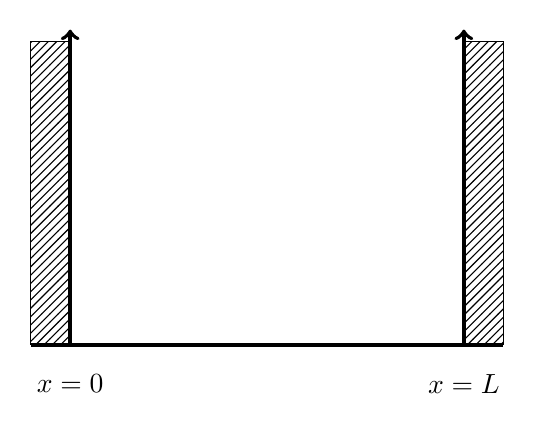
\begin{tikzpicture}
\draw [-to, line width = 0.5mm] (-2.5,0) -- (-2.5,4);
\draw [-to, line width = 0.5mm] (2.5,0) -- (2.5,4);
\draw [line width = 0.5mm] (-3,0) -- (3,0);
\draw[thin,pattern={north east lines}, pattern color= black] (3,0) rectangle (2.5,3.85);
\draw[thin,pattern={north east lines}, pattern color= black] (-2.5,0) rectangle (-3,3.85);
\node at (-2.5, -0.5) {$x=0$};
\node at (2.5, -0.5) {$x=L$};
\end{tikzpicture}
\end{center}
At the shaded regions the potential is defined to be infinite. But between positions $x=0$ and $x=L$ it is defined as $V(x)=0$. Due to the fact that the energy of a particle must be greater than the potential it is experiencing, we have two conditions that within the well it must have positive energy, and outside its wavefunction must vanish, so the lines $x=0$ and $x=L$ act as hard walls which bind the state to being between positions $0$ and $L$.
\\\\
We can list the properties of the system given by the boundary conditions:
\begin{enumerate}
    \item $\Psi(x)$ does not exist if $x>L$ or $x<0$. 
    \item The new normalisation requirement for the system $\Psi$ is $\sip{\Psi}=1=\int_{0}^{L} \Psi^\ast(x)\Psi(x)\,dx$. This is because the boundary conditions require that the probability of the wavefunction being between $0$ and $L$ is $1$, not simply just the probability that it is between negative infinity and infinity.
\end{enumerate}
\\
We know that the wavefunction is continuous. This means actually that it must vanish at the walls $x=0$ and $x=L$, or otherwise it couldn't drop to $0$ straight afterwards. So $x=0$ and $x=L$ are \apos{hard} walls. In other words,
$$
\Psi(0) = 0 = \Psi(L) 
$$
\\
Finally, within the region $x\in(0,L)$, we have $V(x)=0$. Thus the problem reduces to the free particle inside the square well. 
\\\\
We split the problem into three components: the first, investigating the wavefunction inside the well, the second, investigating the wavefunction outside the well, and finally, investigating the wavefunction on the boundary lines $x=0$ and $x=L$; we will cover these in that order.
\\\\
The first part of the problem, the problem of the wavefunction inside the square well, is simply the free particle problem since the potential is $0$, within finite position bounds. So, we once again have
$$
\frac{d^2\Psi}{dx^2} = -{\frac{2mE}{\hbar^2}}\Psi
$$
which has the solution
$$
\Psi(x)=Ae^{ikx}+Be^{-ikx}
$$
for some constants $A,B$, where 
$$
k=p/\hbar=\frac{\sqrt{2mE}}{\hbar}.
$$
We cannot yet determine these constants $A,B$ until we look at the other boundary conditions.
\\\\
The second component of the problem is the problem of the wavefunction outside the well. We recall that the wavefunction
$$
\Psi(x)
$$
is a probability distribution function which returns a value given a position $x$ which is its component in the basis and therefore a probability amplitude for achieving that measurement of $x$. Given that outside the well we have infinite potential, we must have probability zero of finding the particle there. This means that the solution of the wavefunction must also be 
$$
\Psi(x)=0 \mtab \forall x\in(-\infty,0)\cup(L,\infty)
$$
\\
The most important part of the problem comes, however, with the third component of the problem- that of the wavefunction on the hard walls $x=0$ and $x=L$. We have
$$
\Psi(x) = Ae^{ikx}+Be^{-ikx}
$$
for some constants $A$ and $B$. We can rewrite this with Euler's formula:
$$
\begin{aligned}
e^{ix}&=\cos(x)+i\sin(x)\\
\implies Ae^{ikx}+Be^{-ikx}&=A\cos(kx)+iA\sin(x)+B\cos(-kx)+iB\sin(-kx).
\end{aligned}
$$
The cosine function is even and the sine function is odd. Therefore we have 
$$
Ae^{ikx}+Be^{-ikx}=(A+B)\cos(kx)+i(A-B)\sin(kx).
$$
Now, examining the wall conditions, we firstly have:
$$
\Psi(x=0) = 0 
$$
\\
But since $\sin(0)=0$ this means 
$$
(A+B)\cos(kx)=(A+B)\cos(0)=0.
$$ 
However, $\cos(0) \neq 0 $. Therefore we must conclude that $A+B=0$. However, if we conclude this fact then it must be true for all regions, not simply just the wall $x=0$, as the wavefunction cannot simply morph as soon as it reaches $x=0$. Thus for the wavefunction of the whole problem of the infinite square well, which we will now be covering in trigonometric form, we can omit the first coefficient entirely and therefore vanish the cosine term. We are left with
$$
\Psi(x) = i(A-B)\sin{kx}.
$$
\\
Note that we have 
$$
A+B=0
$$
so neither of the individual constants $A$ and $B$ can be $0$, or that would imply the other is $0$, and we would have (in exponential form)
$$
\Psi(x)=0e^{ikx}+0e^{-ikx}=0
$$
which is absurd.
%Haha! It's not absurd, because it's a perfectly good solution to the problem: a zero wave. The word for such a solution is ``trivial'', i.e. not absurd but quite the opposite: uninteresting!
Now we can use the other boundary condition.
$$
\psi(x=L)=0 \Rightarrow\:\: i(A-B)\sin{kL}=0.
$$
\\
If we had 
$$
A-B=0
$$
then we would have 
$$
A-B=A+B=0 \implies B=0 \implies A=0
$$
which is impossible as shown above. Therefore we must have 
$$
\sin(kL)=0.
$$
This means that we must have $kL=n\pi, \:\: n \in \mathbb{Z}$. This means the wave number $k$ is again quantized! Thus we can define.
$$
k_n=\frac{n\pi}{L}
$$
which therefore means we have discrete momenta:
$$
p_{n}=\hbar k_{n}=\frac{n\pi\hbar}{L}
$$
and discrete energy:
$$
E_{n}=\frac{p_{n}^2}{2m}=\frac{\hbar^2\pi^2 n^2}{2mL^2}\stab.
$$
Plugging in to our original general solution for the wavefunction, we have the complete set of solutions 
$$
\Psi_{n}(x)=N\sin\left(\frac{n\pi x}{L}\right).
$$
The constant $N$ is a normalisation constant, which incorporates $i(A-B)$, which we had before. It must be remembered that $A$ and $B$ are arbitrary constants which really are not very important, so rolling them into a new constant $N$ is not a big problem. We can restrict ourselves to considering $n \in \mathbb{Z}^+$ since the parity of the wavefunction is irrelevant in producing the same results. This time, we will solve for the normalisation constant $N$.
$$
\int_{0}^{L}\Psi^\ast(x)\Psi(x)\,dx = N^2\int_{0}^{L}\sin^2\left(\frac{n\pi x}{L}\right) \,dx
$$
since the sine function is real valued so its complex conjugate is itself. Then,
$$
N^2\int_{0}^{L}\sin^2\left(\frac{n\pi x}{L}\right) \,dx = 1
$$
\\
The integral requires some algebra to evaluate. Using the trigonometric identity $\sin^2{kx}=\frac{1-\cos{2kx}}{2}$, we get:
$$
\begin{aligned}
&\sin^2{kx}=\frac{1-\cos{2kx}}{2}\\
\Rightarrow\:\: &\int_{0}^{L}\sin^2{kx}=\int_{0}^{L}\frac{1-\cos{2kx}}{2}\\
\Rightarrow\:\: &\int_{0}^{L}\sin^2{kx}=\int_{0}^{L}\frac{1}{2}-\int_{0}^{L}\frac{1}{2}{\cos{2kx}}\\
\Rightarrow\:\: &\int_{0}^{L}\sin^2{kx}=\int_{0}^{L}\frac{d}{dx}\left(\frac{1}{2}x+c\right)-\frac{1}{2}\int_{0}^{L}\frac{d}{dx}\left({\frac{1}{2k}\sin{2kx}}\right)\\
\Rightarrow\:\: &\int_{0}^{L}\sin^2{kx}=\biggl[\frac{1}{2}x+c\biggr]_{0}^{L}-\biggl[\frac{1}{2k}\sin{2kx}\biggr]_{0}^{L}\\
\Rightarrow\:\: &\int_{0}^{L}\sin^2{kx}=\frac{L}{2}-\biggl[\frac{1}{2k}\sin{2kx}\biggr]_{0}^{L}\\
\end{aligned}
$$
%You'd render the above algebra clearer by cutting out the implies sign and the integral on lines 3,4,5,6, and aligning the = signs, in a similar manner to the algebra below.
\\
Now, plugging in $k=\frac{n\pi}{L}$, we get:
$$
\begin{aligned}
\int_{0}^{L}\sin^2\left(\frac{n\pi x}{L}\right) \,dx &= \frac{L}{2}-\biggl[\frac{L}{n\pi}\sin\left(\frac{2n\pi a}{L}\right)-\frac{1}{2k}\sin{0}\biggr]\\
&=\frac{L}{2}-\biggl[\frac{L}{n\pi}\sin{2n\pi}-0\biggr]\\
&=\frac{L}{2}
\end{aligned}
$$
\\
since $\sin{2n\pi}=0$. So for the normalisation constant we have evaluated the integral from $0$ to $L$ and get:
$$
N^2\int_{0}^{L}\sin^2\left(\frac{n\pi x}{L}\right) \,dx=\frac{N^2L}{2}=1 \Rightarrow\:\: N=\sqrt{\frac{2}{L}}
$$
as our normalisation constant. That gives us the following set of normalised solutions indexed by positive integers $n$:
$$
\Psi_n=\sqrt{\frac{2}{L}}\sin\left(\frac{n\pi x}{L}\right).
$$
We can confirm these are orthogonal to each other for different $n$ and thus create an orthonormal set. The normalised property is covered by the normalisation coefficient $\sqrt{{2}/{L}}$, and the orthogonality can be proved by considering the inner product- from $x=0$ to $x=L$ since this is the domain of the wavefunction without it vanishing.
    $$
    \begin{aligned}
    \int_{0}^{L} \psi^\ast_m(x)\psi_n(x) \,dx = \left(\sqrt{\frac{2}{L}}\right)^2\int_{0}^{L}\sin\left(\frac{m\pi x}{L}\right)\sin\left(\frac{n\pi x}{L}\right)\,dx
    \end{aligned}
    $$
    \\
    since the complex conjugate of the real valued sine function is itself. Then:
    $$
    \begin{aligned}
    \sin{x}\sin{y}&= \frac{1}{2}[\cos(x-y)+\cos(x+y)]\\
    &\Rightarrow\:\: \frac{2}{L}\int_{0}^{L}\sin\left(\frac{m\pi x}{L}\right)\sin\left(\frac{n\pi x}{L}\right)\,dx\\
    &=\frac{2}{L}\int_{0}^{L}\frac{1}{2}\biggl[\cos\left(\frac{(m-n)\pi x}{L}\right)+\cos\left(\frac{(m+n)\pi x}{L}\right)\biggr]\\
    &= \frac{1}{L}\int_{0}^{L}\biggl[\cos\left(\frac{(m-n)\pi x}{L}\right)+\cos\left(\frac{(m+n)\pi x}{L}\right)\biggr]\\
    \end{aligned}
    $$
    \\
    Using some chain rule:
    $$
    \frac{d}{dx}\sin\left(\frac{(m-n)\pi x}{L}\right)= \frac{d}{dg}\sin(g(x))*\frac{d}{dx}\frac{(m-n)\pi}{L}x
    $$
    \\
    where $g(x) = \frac{(m-n)\pi}{L}x$. Then this means:
    $$
    \frac{d}{dx}\sin\left(\frac{(m-n)\pi x}{L}\right)=\frac{(m-n)\pi}{L}\cos\left(\frac{(m-n)\pi}{L}x\right)
    $$
    And therefore,
    $$
    \cos\left(\frac{(m-n)\pi}{L}x\right)= \frac{L}{(m-n)\pi}\frac{d}{dx}\sin\left(\frac{(m-n)\pi x}{L}\right)
    $$
    \\
    so we doing something similar with the $\cos(\frac{(m+n)\pi x}{L})$ term we can write the integral as:
    $$
    \frac{1}{L}\int_{0}^{L}\biggl[\left(\frac{L}{(m-n)\pi}\right)\frac{d}{dx}\sin\left(\frac{(m-n)\pi}{L}x\right)+\left(\frac{L}{(m+n)\pi}\right)\frac{d}{dx}\sin\left(\frac{(m+n)\pi}{L}x\right)\biggr]
    $$
    \\
    then, pulling out constants and using the fundamental theorem of calculus to get rid of the integral, we get the expression
    $$
    \biggl[\frac{1}{(m-n)\pi}\sin\left(\frac{(m-n)\pi}{L}x\right)+\frac{1}{(m+n)\pi}\sin\left(\frac{(m+n)\pi}{L}x\right)\biggr]_{0}^{L}
    $$
    \\
    clearly at $x=0$ we get a bunch of $\sin(0)$ terms so the large bracket is 0. At $x=L$ the value of $x$ cancels with the denominator inside the sine function, and so we get the sine values of $m-n\in\mathbb{Z}^{+}$ lots of $\pi$, which also ends up with 0. So altogether we have proved the whole integral and therefore the inner product of $\Psi_m$ and $\Psi_n$ is $0$. Note that the whole process is invalid when $m=n$ since then the fraction $\frac{L}{(m-n)\pi}$ we see in the expression of $\cos(\frac{(m-n)\pi}{L}x)$ as a derivative is clearly invalid due to division by $0$. Now we can summarise:
    $$
    \ip{\Psi_{m}}{\Psi_{n}} = \delta_{n,m}
    $$
    which is our original definition of an orthogonal set of wavefunctions $\ket{\Psi}$. So indeed, the set of $\Psi_{n}$ indexed by integers $n$ is an orthonormal set of states which can then be linearly combined into any superposition of states with different probabilities.
\subsubsection{Analysing solutions}
We can summarise our numerical analysis of eigenstates as follows. We obtained:
$$
\psi_n=\sqrt{\frac{2}{L}}\sin(\frac{n\pi x}{a}), \:\:\:\:\: E_n=\frac{\hbar^2\pi^2 n^2}{2ma^2}, \:\:\:\:\: n \in \mathbb{Z}^+
$$
\\\\
We can now plot the first $\psi_n$ on an axis from $0$ to $a$. This is in shown in figure 1.
%Is there a figure 1.???
Clearly, we observe a few properties:
\begin{enumerate}
    \item We call a zero of $\psi$ inside the domain of $\psi$ a node. Then here we see that $\psi_n$ has $n-1$ nodes: the zeros at $x=0$ and $x=a$ do not count as they are not inside the domain. More importantly, for this set of solutions to $\psi$ for every $1$ that you increase the integer indexing $\psi_n$ you also increase the number of nodes by $1$. This is actually generally true as you go up from the ground state- the lowest energy state and nearly always $\psi_1$ in a set of $\psi_n, \:\: n \in \mathbb{Z}^+$: for any set of solutions $\psi$ we add 1 node every time we move to the next possible energy level.
    \\
    \item The $\psi_n$ are clearly alternately symmetric and asymmetric as you go up index numbers $n$. $\psi_1$ is symmetric, $\psi_2$ is asymmetric, $\psi_3$ is symmetric, etc. Crucially, we call symmetric solutions \textbf{even} and the asymmetric solutions \textbf{odd}. The definition of an even function $f(x)$ is that $f(x)=f(-x)$. The definition of an odd function is where $f(-x)=-f(x)$. Technically here there are neither even solutions nor odd solutions since this is not true for any $\psi_n$ in the question defined. But if we had taken the midpoint of the well to be $x=0$ then looking at the first few wavefunctions it is clear this would have been true, so the parity of functions we think in is analogous. We will see in our next problem how important discussion of function parity will be in breaking down questions as they get more and more complex and we seek to categorise more and more realistic situations and problems. But there exists a powerful fact: if a particle is in an even potential then all wavefunctions are either odd or even. In this problem again if we had set the middle of the potential well to be $0$ then we would have seen an example of this fact: the potential would be even since it is symmetric about $0$ and the solutions are alternately even and odd. Clearly this is an exceptionally meaningful fact. We can prove it fairly easily for our one-dimensional purposes:
    $$
    \text{By Schrodinger}, \:\: -{\frac{\hbar^2}{2m}\frac{d^2}{dx^2}}\psi(x)+V(x)\psi(x)=E\psi(x)
    $$
    \\
    when we substitute in $x=-x$, we get:
    $$
    -{\frac{\hbar^2}{2m}\frac{d^2}{dx^2}}\psi(-x)+V(-x)\psi(-x)=E\psi(-x)
    $$
    \\
    we are considering a question where the potential is even and thus $V(x)=V(-x)$ So then:
    $$
    -{\frac{\hbar^2}{2m}\frac{d^2}{dx^2}}\psi(-x)+V(x)\psi(-x)=E\psi(-x)
    $$
    \\
    we step back out of the algebraic manipulation and see that clearly this means that if $\psi(x)$ is a solution in an even potential then $\psi(-x)$ is also a solution. This in itself is very important, naturally. But since we are working in the same one-dimensional vector space of solutions to the same Schrodinger then it is impossible for these two functions to be linearly independent, or orthogonal in a one-dimensional space. Therefore we can say
    $$
    \psi(x)=a\psi(-x)
    $$
    \\
    for some constant $a$. Then $a\psi(-x)=\psi(x)$, so it satisfies the conditions, and therefore is normalised. So we have:
    $$
    |a|^2\int_{-\infty}^{\infty}\psi^{\ast}(-x)\psi(-x)\,dx=1
    $$
    \\
    But $\psi(-x)$ itself is a normalised solution so the integral is equal to 1. Therefore 
    $$
    |a|^2=1 \Rightarrow\:\:\:\: a=\pm1
    $$
    By definition when $a=1$ then $\psi$ is even since we get $\psi(x)=\psi(-x)$, and when $a=-1$ then $\psi$ is odd, since we get $\psi(x)=-\psi(x)$. Therefore for an even potential all solutions $\psi$, when normalised, must be even or odd.
\end{enumerate}
\section{Harmonic Oscillator \ast}
We now introduce a third less fundamental but perhaps more impactful problem which must be included in any discussion of quantum mechanics. We will take one system we know very well from classical mechanics, the spring, which has a potential of 
$$
V(x)=\frac{1}{2}kx^2
$$
for the spring constant $k$. This can also be written via the angular frequency, $\omega=k/m$, as 
$$
V(x)=\frac{1}{2}mX\omega^{2}.
$$
There is the standard method of solving this problem in the quantum mechanical version, where the Hamiltonian is 
$$
\hat{H}=\frac{\hat{P}^2}{2m}+\frac{1}{2}m\hat{X}^{2}\omega^{2}.
$$
We note that for the system the spring constant and mass are both constants, and so $\omega=k/m$ is a constant and therefore should not and cannot be replaced by an expression in the position and momentum operators for the quantum Hamiltonian. Now the conventional method would be to solve the problem in position space and implement strategies much like we have shown above. But there is a method, courtesy of Dirac, which shows that we can use the energy eigenbasis as well.
\\\\
In principle this should be difficult, as to find the energy eigenkets which form the energy eigenbasis is tantamount to solving for the propagator for time evolution, in which case it is unclear why we would ever need to be in the energy eigenbasis after that. However, elegance will show in a clever way this limitation is not quite concrete for all problems, and the energy eigenbasis can be very useful even before we know the eigenvectors.
%This last section 8.4 needs some sorting out! It starts entitled Harmonic Oscillator, for which you then introduce the counting operator, and thence creation and destruction operators. But, as far as I can tell, none of that has been related back to the harmonic oscillator, which you mention and then forget about. 
%I think it would be much better to entitle and introduce this last section as the road to quantum field theory, which is what almost all of it is.
\\\\
To start, we define the operator
$$
a=\sqrt{\frac{m\omega}{2\hbar}}\left(\hat{X}+\frac{i\hat{P}}{m\omega}\right).
$$
Then we consider its hermitian adjoint,
$$
a^{\dagger}=\sqrt{\frac{m\omega}{2\hbar}}\left(\hat{X}-\frac{i\hat{P}}{m\omega}\right).
$$ 
It is clear these operators are not hermitian. What relationship is held by the two operators? They turn out not to be unitary either. Instead, we get 
$$
[a,a^{\dagger}]=1
$$
which can be easily verified:
$$
\begin{aligned}
[a,a^{\dagger}]&=\frac{m\omega}{2\hbar}\left[\biggl(\hat{X}+\frac{i\hat{P}}{m\omega}\biggr)\biggl(\hat{X}-\frac{i\hat{P}}{m\omega}\biggr)\right]-\frac{m\omega}{2\hbar}\biggl[\left(\hat{X}-\frac{i\hat{P}}{m\omega}\right)\left(\hat{X}+\frac{i\hat{P}}{m\omega}\right)\biggr]\\
&=\frac{m\omega}{2\hbar}\biggl[\hat{X}^{2}-\frac{i}{m\omega}[\hat{X},\hat{P}]-\left(\frac{i\hat{P}}{m\omega}\right)^2-\hat{X}^2-\frac{i}{m\omega}[\hat{X},\hat{P}]+\left(\frac{i\hat{P}}{m\omega}\right)^2\biggr]\\
&=\frac{m\omega}{2\hbar}\biggl[-\frac{i}{m\omega}(2i\hbar)\biggr]=\frac{m\omega}{2\hbar}\frac{2\hbar}{m\omega}=1
\end{aligned}
$$
Finally, we can define an operator, $N$, to be $a^{\dagger}a:=N$. This operator is hermitian as $a^{\dagger}a$.
%Needs a little tweak.
This operator has the form, as seen above:
$$
\begin{aligned}
N&=\frac{m\omega}{2\hbar}\biggl[\hat{X}^2+\frac{i}{m\omega}[\hat{X},\hat{P}]-\left(\frac{i\hat{P}}{m\omega}\right)^2\biggr]=\left(\frac{m\omega}{2\hbar}\right)\left[\hat{X^2}+\frac{\hat{P}^2}{m^2\omega^2}+\frac{i}{m\omega}[\hat{X},\hat{P}]\right]\\
&=\frac{1}{\hbar\omega}\frac{\hat{P}^2}{2m}\frac{1}{2\hbar}+{\hat{X}^2}m\omega+\frac{i}{2\hbar}i\hbar
\end{aligned}
$$
Regarding the Hamiltonian of the system again, this is 
$$
N=\frac{\hat{H}}{\hbar\omega}-\frac{1}{2}\implies\hat{H}=\hbar\omega\left(N+\frac{1}{2}\right).
$$
A bit of clever compatibility thinking is again the step here. Technically $N$ is not an observable operator, but note that what we proved about compatible observables did not hinge on the fact that the operators were Hermitian or had real eigenvalues. Only the third component, that about successive measurements of different observables and whether or not they affect the eigenstate, was contingent on the discussion being about observables in the other place.
%I didn't understand this last sentence.
In other words, if two operators commute they possess a common eigenbasis; this is not simply limited to observable operators, as a review of the proof we gave will show.
\\\\
We have seen above that the operator $N$ is a linear combination of the Hamiltonian. This means that they will commute. This in turn means that they possess a common eigenbasis! Thus there exist energy eigenkets $\ket{E}$ which are also eigenkets of the operator $N$. Thus we have the relationship
$$
\hat{H}\ket{E}=E\ket{E}
$$
as usual, but also the relationship
$$
N\ket{E}=n\ket{E}
$$
for some eigenvalue $n$. We can now equate the eigenvalues!
$$
\hat{H}\ket{E}=\hbar\omega\left(N+\frac{1}{2}\right)\ket{E}=\hbar \omega N\ket{E}-\frac{\hbar\omega}{2}\ket{E}=\hbar\omega\left(n+\frac{1}{2}\right)\ket{E}
$$
So the energy eigenvalues are given by 
$$
E_{n}=\left(n+\frac{1}{2}\right)\hbar\omega.
$$
The author has tried to instil a justified suspicion in the reader for indexing by $n$ without knowing there is a discrete case which can be indexed by integers; indeed, we still do not know anything about the eigenvalues $n$ so energy could still well be continuous at this stage, and indexing by $n$ would be meaningless. However, we will soon prove that in this case this step is fine as the eigenvalues of $N$ are in fact nonnegative integers $n$! We will from now on refer to $N$ as the counting operator, as is widespread convention. Let us consider some more commutation relations.
\\\\
By the commutation relation 
$$
[AB,C]=A[B,C]+[A,C]B
$$
we have
$$
[N,a^{\dagger}]=[a^{\dagger}a,a^{\dagger}]=a^{\dagger}[a,a^{\dagger}]+[a^{\dagger},a^{\dagger}]a=a^{\dagger}(1)+0=a^{\dagger}.
$$
Now we also have
$$
[N,a^{\dagger}]=Na^{\dagger}-a^{\dagger}N\implies Na^{\dagger}=a^{\dagger}N+[N,a^{\dagger}]=a^{\dagger}N+a^{\dagger}.
$$
Thus applying the operator to an energy eigenket, now indexed by $n$,
$$
Na^{\dagger}\ket{E_{n}}=(a^{\dagger}N+a^{\dagger})\ket{E_{n}}=a^{\dagger}N\ket{E_{n}}+a^{\dagger}\ket{E_{n}}=(n+1)a^{\dagger}\ket{E_{n}}.
$$
The reader will recognise the above as another eigenvalue equation, which states that for the counting operator, we have 
$$
N\ket{E_{n}}=n\ket{E_{n}}
$$
as one eigenvalue equation, but also the ket $a^{\dagger}\ket{E_{n}}$ as an eigenket which has an eigenvalue $n+1$ such that as above, the equation
$$
N(a^{\dagger}\ket{E_{n}})=(n+1)(a^{\dagger}\ket{E_{n}})
$$
applies. We have mentioned that $n$ is a nonnegative integer, so what this is really saying is that if we apply the counting operator $\ket{E_{n}}$, we get the \apos{measurement} of an eigenvalue $n$, but if we then change the eigenket by applying the operator $a^{\dagger}$ to it first, and then apply the counting operator, we will now count the eigenvalue $n+1$. What is the physical meaning of $n$? Well, we have 
$$
E_{n}=\left(n+\frac{1}{2}\right)\hbar\omega.
$$
The meaning of $\hbar\omega$ is interesting: one unit we can choose for the Planck's constant $\hbar$ is joules per hertz, and the angular frequency, as suggested by the name, can be measured in hertz, which means that units of $\hbar\omega$ are measured in joules- thereby a measure of energy. Of course, the value of $\hbar\omega$ is not $1$ Joule, since the angular frequency would have to be unthinkable for this to be true, but we can think of $\hbar\omega$ as small \apos{packets} of energy (in a loose intuitive manner) which we can use to measure the energy of the system it turns out very appropriately on the microscopic scale. The basic analogy one has already seen in their own studies? Coulombs as a measure of charge, which are also technically \apos{packets} of electrons (again in a very loose manner) which help make the counting process easier!
\\\\
Thus every time we increase $n$ we increase the energy reading. When $n$ is measured that corresponds to when the counting operator acts on the energy eigenket $\ket{E_{n}}$, and the corresponding energy is $n+1/2$ in units $\hbar\omega$. However, if we apply $a^{\dagger}$ to $\ket{E_{n}}$ first, we replace $n$ with $n+1$, thereby replacing the corresponding energy $n+1/2$ with the energy $n+1+1/2$. Thus the operator $a^{\dagger}$ \textbf{creates} one unit of energy, measured in $\hbar\omega$- giving it is name. Similarly:
$$
[N,a]=[a^{\dagger}a,a]=a^{\dagger}[a,a]+[a^{\dagger},a]a=a^{\dagger}(-1)+0=-a.
$$
Now we also have
$$
[N,a]=Na-aN\implies Na=aN+[N,a]=aN-a.
$$
Thus applying the operator to an energy eigenket, now indexed by $n$,
$$
Na\ket{E_{n}}=(aN-a)\ket{E_{n}}=aN\ket{E_{n}}-a\ket{E_{n}}=(n-1)a\ket{E_{n}}.
$$
Which, by the same argument as above, shows that the operator $a$ acting on a energy eigenstate $E_{n}$ \textbf{annihilates} (dramatic, but conventional) one unit of energy $\hbar\omega$! Thus the names the creation operator for $a^{\dagger}$ and the annihilation operator for $a$.
\\\\
Next, we wonder if there is an easier way to label the kets $a^{\dagger}\ket{E_{n}}$ and $a\ket{E_{n}}$, which we have also noted are eigenkets of the counting operator. Well, of course there is-
$$
N\ket{E_{n+1}}=(n+1)\ket{E_{n+1}}, \btab Na^{\dagger}\ket{E_{n}}=(n+1)a^{\dagger}\ket{E_{n}}\implies a^{\dagger}\ket{E_{n}}\equiv \ket{E_{n+1}}.
$$
This is completely reasonable, because $a^{\dagger}$ on the state $\ket{E_{n}}$ raises the energy by $1$. However, by the formula
$$
E_{n}=\left(n+\frac{1}{2}\right)\hbar\omega,
$$
and the fact we have taken it as a given that $n\in\mathbb{Z}^{+}$, we must have $E_{n+1}=E_{n}+1\times\hbar\omega$, in which case the equivalence of the states $a^{\dagger}\ket{E_{n}}$ and $\ket{E_{n+1}}$ makes perfect sense. Similarly, of course, $a\ket{E_{n}}$ and $\ket{E_{n-1}}$ are equivalent states. Yet we know that equivalence is not algebraic equality: rather,
$$
a\ket{E_{n}}=c\ket{E_{n-1}}
$$
for some multiplicative constant $c$ is sufficient for them to be equivalent states. The norm of $a\ket{E_{n}}$ is 
$$
\nhoptrip{E_{n}}{a^{\dagger}\:a}{E_{n}}=\nhoptrip{E_{n}}{N}{E_{n}}
$$
by our correspondence 
$$
\Omega\ket{X}\duac\bra{X}\Omega^{\dagger}.
$$
This is then equal to 
$$
|c|^2\sip{E_{n-1}}=|c|^2
$$
given the definition of $c$ above and the assumption that $\ket{E_{n+1}}$ has already been normalised. So we have 
$$
\nhoptrip{E_{n}}{N}{E_{n}}=n\sip{E_{n}}=n=|c|^2\implies c=\sqrt{n}.
$$
Thus we have 
$$
a\ket{E_{n}}=\sqrt{n}\ket{E_{n-1}}.
$$
We can do the exact same thing for $a^{\dagger}$ to get 
$$
a^{\dagger}\ket{E_{n}}=\sqrt{n+1}\ket{E_{n+1}}. 
$$
By the semidefinite metric, the norm of any ket, including $a\ket{E_{n}}$ is positive. However, the norm of $a\ket{E_{n}}$ is $n$ as already shown. Thus, $n$ must be nonnegative. We next realise that all we have covered so far means that
$$
(a^{2})\ket{E_{n}}=a\sqrt{n}\ket{E_{n-1}}=\sqrt{n}a\ket{E_{n-1}}=\sqrt{n(n-1)}\:\ket{E_{n-2}}
$$
and so on- in other words, applying the annihilation operator means we should be able keep annihilating energy in units of $\hbar\omega$ until we reach a negative value of $n$, no matter how great the $n$ and therefore energy. The reason this is problematic, however, is that we have already proven that the counting operator eigenvalue $n$ corresponding to the energy and counting simultaneous eigenstate $\ket{E_{n}}$ must be nonnegative due to the semidefinite postulate. So we cannot expect a negative value of $n$ to appear. As we have 
$$
a\ket{E_{n}}=\sqrt{n}\ket{E_{n-1}}
$$
We conclude that if we reach a $E_{n}$ with $n<0$ the definition means we must have reached an eigenvalue $n<0$. The fact above with the sequence of square roots shown by repeatedly applying the annihilation operator shows that clearly we should be able to reach a state $E_{n}$ with $n<0$. This is unless we terminate at a value before we reach below $n=0$. If after annihilating a sufficient number of $\hbar\omega$ units of energy we had $n\in(0,1)$ then we would be able to apply the annihilation operator again to get a new $n'=n-1\in(-1,0)$ which is negative. If we had a value of $n>1$ which was not an integer then we conclude we must be able to keep applying the annihilation operator until we get a value in the region $(0,1)$, after which the same argument applies that we reach a negative $n$. Thus we must have the value $n=1$ occurring, after which reapplying the annihilation operator should give $n=0$. What if we now try to reapply the annihilation operator? Well then, we have
$$
a\ket{E_{n}}=\sqrt{n}\ket{E_{n-1}}\implies a\ket{E_{0}}=0\ket{E_{-1}}=0.
$$
In other words, all negative index $E_{n}$, and therefore negative $n$ disappear! This satisfies our condition of being able to apply the annihilation operator repeatedly but not ever having states where the counting operator eigenvalue $n$ is negative. Thus we have shown with this argument, which should be reread if one is not convinced, that all we have done thus far on the assumption that the eigenvalues $n$ are integers was done on the correct assumption: $n$ must be a nonnegative integer, and there is a terminating state $\ket{E_{0}}$ which has energy $E_{0}=(0+1/2)\hbar\omega=(1/2)\hbar\omega$.
\chapter{Appendix: A Mathematical Toolbox}
This book is designed so that even high schoolers can access quantum mechanics. As such, this section is a reference section, which acknowledges the fact that high school curricula might teach different topics in slightly different orders and detail, and also that some of the prerequisite mathematics assumed here might be just a small reach beyond high school syllabus. The reference section contains some instruction, but it should not be used for anyone learning these topics for the first time, as I have been quite brief so as not to distract from the main topic of this book. For those who are unfamiliar with using any of the mathematical rules referenced as assumed knowledge, they should turn to any textbook which covers these topics and complete a thorough run through some exercises before reading any other part of this book. For many other students, they can simply look at the exercises in these sections, and if they do not see anything unfamiliar, they can simply skip this reference chapter.
\\\\
\section{Mathematical Syntax}
There are multiple symbols used as figures of proof in this book, which represent common phrases one might turn to were they reciting a proof out loud. As these are ubiquitous symbols, being fluent reading them will be necessary, as otherwise they can be especially easy to confuse with each other.
\\\\
\begin{tabular}{| c | c |}
\hline
 \textbf{Symbol} & \textbf{Meaning} \\ 
 \hline
 $:=$ & `define equals'\\
 \hline
 $\forall$ & `For all' \\
 \hline
 $\exists$ & `There exists'\\
 \hline
 $\in$ & `In' (for a set)\\
 \hline
 $\implies$ & `Implies' \\
 \hline
 $\iff$ & `Implies each other' \\
 \hline
`Iff' & `If and only if' \\
\hline
 $\sum_{i\neq j}$ & `Sum over all $i$ not equal to $j$' \\
 \hline
 $\sum_{\{i\}}$ & `Sum over all $x$ in a set $\{x\}$'\\
 \hline
 $\square$ & Q.E.D \\
 \hline
 $f'(x)$ & First Derivative of $f(x)$ \\
 \hline
 $f''(x)$ & Second Derivative of $f(x)$\\
 \hline
 $\setof{x_{i}}$ & `the set of values $x_{i}$'\\
 \hline
 $x\to y$ & `x approaches y'\\
 \hline
 $\mathbb{Z}$ & the set of all integers \\ 
 \hline
 $\mathbb{R}$ & the set of all real numbers \\
 \hline
 $\mathbb{Z}^{+}$ & the set of all positive integers \\
 \hline
 $\equiv$ & `is equivalent to'\\
 \hline
\end{tabular}
\\\\
Fluency with basic summation and product notation is assumed. There is also interval notation commonly used for inequalities:
\begin{itemize}
    \item $x\in[a,b)\iff a\leq x < b$
    \item $x\in(a,b]\iff a< x \leq b$
    \item $x\in(a,b) \iff a< x< b$
    \item $x\in [a,b] \iff a \leq x \leq b$
\end{itemize}
and round brackets are always used for any side of the inequality bounded by $\pm \infty$.
\section{Probability$\ast$}
In this book, as correct and conventional, probabilities are numbers between $0$ and $1$, sometimes represented by fractions. 

For a random $X$ variable which can take multiple values $x_{i}$
\section{Complex Numbers$\ast$}
Define the imaginary unit, $i$, to be equal to the square root of $-1$. We then have:
\begin{itemize}
    \item $i^2= (\sqrt{-1})^2=-1$
    \item $\forall\stab k \in \mathbb{R}, \mtab \frac{k}{i}=\frac{ik}{i^2}=\frac{ik}{-1}=-ik$
    \item $\forall\stab k \in \mathbb{R}^+, \mtab \sqrt{-k}\equiv\sqrt{-1} \times \sqrt{k}=i\sqrt{k}$
    \item $\forall\stab a,b \in \mathbb{R}, \mtab ai \pm bi = a\sqrt{-1}\pm b\sqrt{-1}= (a\pm b)\sqrt{-1}=(a\pm b)i$
\end{itemize}
Complex numbers are numbers usually represented in the form 
$$
z:=a+bi
$$
for some $a,b\in\mathbb{R}$. Then there are two functions commonly referred too:
\begin{itemize}
\item $\text{Re}(z)$ is called the `real part' of the imaginary number $z$, which is, the real number $a$ if $z:=a+bi$.
\item $\text{Im}(z)$ is called the `imaginary part' of the imaginary number $z$, which is, the real number $b$ if $z:=a+bi$. Note that $\text{Im}(z)=b$ and not $\text{Im}(z)=bi$. 
\end{itemize}
It is then clear that a real number is also a complex number, but with imaginary part $0$. Conversely, if a complex number has imaginary part $0$, then all that remains is its real part and so it must be a real number. Therefore,
\begin{itemize}
    \item $z \in \mathbb{R} \iff \text{Im}(z)=0$.
\end{itemize}
We may represent any complex number on a real-valued two dimensional plane called an Argand diagram (figure). From this figure we can create a few more useful definitions:
\begin{itemize}
    \item The modulus of a complex number $z$ is denoted $|z|$ and defined to be $|z|:=\sqrt{\text{Re}(z)^2+\text{Im}(z)^2}$. This is the application of Pythagoras' Theorem to find the distance from any point $z$ represented on the Argand diagram to the origin.
    \item For all complex numbers $z:=a+bi$, we denote with $z^{\ast}$ the complex conjugate of the complex number, defined by $z^{\ast}=a-bi$ (in other words, reversing the sign of the imaginary part).
    \item For all complex numbers $z$, we define the modulus squared (or square modulus) of that complex number to be $|z|^{2}:=zz^{\ast}$. This modulus squared is always real.
\subsubsection{Exercises on Complex Numbers*}
\begin{enumerate}
    \item Express as a single complex number with distinct real and imaginary parts:\begin{enumerate}
    \item $(4i)^3$ \\
    \item $(5-7i)(6-8i)$ \\
    \item $\frac{3+5i}{2-4i}$ \\
    \item $(-4-7i)^{\ast}$ \\
    \item $|2+3i|^2$ \\
    \end{enumerate}
    \item Show, with proof, whether each of the following statements are true \begin{enumerate}
        \item $|z|>|\text{Re}(z)|$ and $|z|\geq|\text{Im}(z)|$
        \\
        \item $\forall\stab z\in\mathbb{C}, \mtab |z|^2\in\mathbb{R}$ \\
    \end{enumerate}
    \item Show that $|r\cos\theta+ir\sin\theta|=r$ \\
    \item 
\end{enumerate}
\end{itemize}
\section{Matrices*}
A matrix is an array of values. They are placed into rectangular arrangements in rows and columns, and are an extremely important way of mathematically listing values. We shall see that the structure of a matrix allows for powerful computations to be done. For now, there are many definitions to cover.
\\\\
A matrix with $m$ rows and $n$ columns is said to be an $m\times n$ matrix. A $n\times n$ matrix is called a square matrix, a $n\times 1$ matrix is usually called a column vector, and a $1\times n$ matrix is usually called a row vector. 
\\\\
The values of a matrix are usually called the element of that matrix. For a matrix denoted by any symbol, for example $M$, the notation $M_{ij}$ usually represents the element in the $i$'th row and $j$'th column of the matrix. Therefore, we can show the four usual types of matrices we might often see:
\begin{enumerate}
    \item An arbitrary $m\times n$ matrix:
    $$
    \begin{bmatrix}
        \text{M}_{11} & \text{M}_{12} & \dots &\dots & \text{M}_{1n} \\
        \text{M}_{21} & \ddots & \dots &\dots & \vdots \\
        \vdots & \dots & \ddots & \dots & \vdots \\
        \text{M}_{m1} & \dots & \dots & \dots & \text{M}_{mn} \\
    \end{bmatrix}
    $$
    \item A $n\times n$ square matrix:
    $$
    \begin{bmatrix}
        \text{M}_{11} & \text{M}_{12} & \dots & \text{M}_{1n} \\
        \text{M}_{21} & \ddots & \dots & \vdots \\
        \vdots & \dots & \ddots  & \vdots \\
        \text{M}_{n1} & \dots & \dots & \text{M}_{nn} \\
    \end{bmatrix}
    $$
    \item A $n\times 1$ column vector:
    $$
    \begin{bmatrix}
        \text{M}_{11} \\
        \text{M}_{21} \\
        \vdots \\
        \vdots \\ 
        \text{M}_{n1} \\
    \end{bmatrix}
    $$
    \item A $1\times n$ row vector:
    $$
    \begin{bmatrix}
        \text{M}_{11} &
        \text{M}_{12} &
        \dots &
        \dots &
        \text{M}_{1n} 
    \end{bmatrix}
    $$
\end{enumerate}
As shown in the examples, a variety of dots are used often to show the idea that we can have a large number of unlisted elements between elements explicitly written. This should not be a great worry, since the arrangements of elements in a matrix are always in ordered rows and columns anyway. We now move onto defining the operations:
\begin{enumerate}
    \item Scalar multiplication of a matrix $M$ by a scalar $a$ results in a new matrix $aM$ with each previous element $M_{ij}$ replaced with a new element $aM_{ij}$. So for example,
    $$
    -1\times\begin{bmatrix}
        5 & 4 & -9 \\
        0 & -1 & 6 \\ 
    \end{bmatrix}
    =
    \begin{bmatrix}
        -5 & -4 & 9 \\
        0 & 1 & -6 \\ 
    \end{bmatrix}
    $$
    \item Two matrices can be summed iff they are of the same dimensions. If they are of the same dimensions, the sum of two matrices $M$ and $N$ are obtained by creating a new matrix $S:=M+N$, of the same dimensions, where each new element of the resultant matrix $S_{ij}$ is the result of summing corresponding position elements in $M$: in other words, $\forall\stab i,j,S:=M+N, \mtab S_{ij}=M_{ij}+N_{ij}$. So for example,
    $$
    \begin{bmatrix}
        3 & 2 \\
        -1 & 8 \\
        0 & 5
    \end{bmatrix} + 
    \begin{bmatrix}
        7 & -3 \\
        -1 & 0 \\
        0 & 2 
    \end{bmatrix} = 
     \begin{bmatrix}
        3+7 & 2-3 \\
        -1-1 & 8+0 \\
        0+0 & 5+2 
    \end{bmatrix}= \begin{bmatrix}
        10 & -1 \\
        -2 & 8 \\
        0 & 7
    \end{bmatrix}
    $$
    \item A matrix multiplying another matrix is more complicated. First of all, for two matrices $M$ and $N$ the matrix products $M\times N$ and $N\times M$ are rarely the same: whichever matrix is on the left of the product changes the result. We say that matrix multiplication is non-commutative. The terms left-multiply and right-multiply emerge naturally from this non-commutativity, where left-multiplying a matrix $M$ by a matrix $N$ means performing a matrix multiplication with that matrix $N$ on the left of the multiplication, and vice versa.
    \\\\
    Next, matrix multiplication can only be performed if the number of columns of the matrix on the left are the same as the number of rows of the matrix on the right. If we have an $a\times b$ matrix $M$ and a $c\times d$ matrix $N$, then the product $M\times N$ is only possible if $b=c$. The result can be best memorised by the crude representation:
    $$
    b=c\implies
    (a\times b) \times (c \times d) = (a\times \cancel{b}) \times (\cancel{b} \times d) = a\times d.
    $$
    Here, we get the idea that the `middle two' values when we list the dimensions of the two matrices being multiplied together in the correct order must match up and then are discarded, leaving the number of rows of the left matrix and the number of columns of the right matrix as the dimensions of the resulting matrix after multiplication.
    \\\\
    
\end{enumerate}
\section{Calculus*}
\section{Misc.*}
\end{document}
